\hypertarget{einleitung}{%
\chapter{Einleitung}\label{einleitung}}

\hypertarget{motivation}{%
\section{Motivation}\label{motivation}}

Eingebettete Systeme (Englisch ``embedded Systems'') sind technische
Zusammensetzungen, welche für eine spezifische Funktion entwickelt
werden. Im Gegensatz zu Mehrzwecksystemen (Englisch ``multi-purpose
systems''), wie zum Beispiel einem Personal Computer, welcher in der
Lage ist, diverse Funktionen auszuführen und nicht zwingend an eine
Funktion gebunden ist, dienen eingebettete Systeme einer bestimmten
Logik. Daraus resultieren simplere und auch Ressourcen-sparsamere
Systeme, die wesentlich näher an der Technik und der für den Zweck
nötigen Komponenten und Software entwickelt werden. Systeme können
günstiger zusammengesetzt und Fehlerquellen schneller entdeckt und
behoben werden. Nicht für den Prozess notwendige Komponenten werden gar
nicht erst verwendet. Bei einem Mehrzwecksystem wird akzeptiert, dass
Komponenten und Schnittstellen existieren, die nicht benötigt werden.
Diese verursachen Kosten und können mögliche Fehlerquellen sein.

Dennoch ist die Entwicklung eines solchen Systems nicht banal. Es ist
abzuwägen, welche Komponenten derzeit auf dem freien Markt erhältlich
sind, welche Funktionen diese mitbringen oder ermöglichen und wie diese
optimal kombiniert werden können. Es bedarf im Vorhinein intensiverer
Recherche und einer größeren Perspektive über mögliche Zusammenhänge. Im
Falle eines Merhzwecksystems ist die Auswahl simpler, da man den Prozess
auch im Nachhinein noch anpassen kann, weil zusätzliche Funktionen und
Komponenten gegeben sind oder leichter ergänzt werden können. Das
eingebettete System muss in der Regel aufgewertet oder sogar völlig
ersetzt werden, wenn zu einem späteren Zeitpunkt festgestellt wird, dass
Funktionen nicht gegeben oder umsetzbar sind. Fertiggestellte Systeme
sind komplexer in der Aufwertung.

Die Fähigkeit zur Erstellung eines solchen System ist daher nicht
leichtfertig anzunehmen und es ist mir wichtig, zum Abschluss meines
Studiums mein gewonnenes Wissen über Systeme, Komponenten, Zusammenhänge
und deren Verbindung bis hin zur Programmierung nachzuweisen. Die
Auswahl eines fertigen Computers oder sogar das simple Nutzen
existierender Betriebssysteme erweckt nicht den gleichen Reiz, wie es
die eigene Erstellung dieser Komponenten auf mich hat. Ich halte es für
essenziell, möglichst fachlich die Inhalte meines Studiums in Verbindung
mit meinen Vorlieben zu bringen, um ein optimales Projekt zu erstellen.

Die Erstellung eines autonomen Schachtischs vereinbart in meinen Augen
im großen Umfang die wesentlichen Komponenten des Informatikstudiums mit
meiner Vorliebe zur mechanisch-elektrischen Gestaltung. Angefangen mit
den Grundlagen der Informatik, insbesondere mit technischem Bezug, über
die Berechnung und Auslegung von Systemkomponenten, zudem die
objektorientierte Projektplanung und Architektur von Systemen bis hin zu
Datenbanken und Webtechnologien und Softwareentwicklung. Zudem wird mein
Studienschwerpunkt, die technische Informatik, mit einem einbetteten
System manifestiert.

Der Reiz im Schachprojekt liegt in der Bedeutung und der Seltenheit.
Schach ist ein bewährtes, ausnahmslos bekanntes und immer logisches
Spiel, welches jedoch im kommerziellen Rahmen nie an Bedeutung gewonnen
hat. Die Auswahl der verfügbaren elektrifizierten und
programmgesteuerten Schachtische ist auffallend gering; zudem sind
existierende Lösungen oftmals nicht erschwinglich und bedürfen
erhebliche Anpassungen des Spielers an das Spiel. Innerhalb der
vergangenen drei Jahrzehnte bewiesen sich immer mehr Konzerne ihre
technische Kompetenz und Überlegenheit und die Fähigkeit ihrer Maschinen
mittels der Auswertung von Schachalgorithmen und dem möglichst schnellen
besiegen derzeitiger Schach-Meister und -Meisterinnen. Die Algorithmen
stehen heute in einer Vielzahl als open-source Projekte zur Verfügung,
jedoch ist das Interesse daran, für Spieler mögliche Anwendungen zu
generieren, verschwindend gering und wird oftmals nur von Experten und
Enthusiasten genutzt und auch hinterfragt.

Mit dieser Arbeit möchte ich mich diesem Problem stellen und einen
möglich günstigen Tisch entwickeln, welcher das Spielerlebnis ohne
Einschränkungen dem Spieler transferiert. Zudem möchte ich gewonnene
Erkenntnisse und aktuelle Ressourcen wie die Cloud-Infrastruktur
einbinden, um das Schachspiel, welches zweier Spieler bedarf, für einen
Spieler zu ermöglichen. Das Ergebnis soll nicht nur viele Zeilen Code
sein, sondern auch ein handfestes Produkt, dass meine Qualitäten und
Enthusiasmus widerspiegeln.

\hypertarget{zielsetzung}{%
\section{Zielsetzung}\label{zielsetzung}}

Das Ziel der nachfolgenden Arbeit ist es, einen autonomen Schachtisch zu
entwickeln, welcher in der Lage ist, Schachfiguren autonom zu bewegen
und auf Benutzerinteraktionen zu reagieren. Darüber hinaus sollte der
autonome Schachtisch weitere folgende Funktionalitäten aufweisen:

\begin{itemize}
\tightlist
\item
  Erkennung Figur-Stellung
\item
  Automatisches Bewegen der Figuren
\item
  Spiel Livestream
\item
  Parkposition für ausgeschiedene Figuren
\item
  Stand-Alone Funktionalität
\end{itemize}

Die Kernfrage der Arbeit bezieht sich somit auf die Überprüfung der
Ausführbarkeit inklusive Erstellung und Umsetzung eines eingebetteten
Systems und einer Cloud-Infrastruktur.

Der Schwerpunkt liegt dabei insbesondere auf der Programmierung des
eingebetteten Systems und dem Zusammenspiel von diesem mit einem aus dem
Internet erreichbaren Servers, welcher als Vermittlungsstelle zwischen
verschiedenen Schachtischen und anderen Endgeräten dient. Dieses besteht
zum einem aus der Positionserkennung und Steuerung der
Hardwarekomponenten (Schachfiguren) und zum anderen aus der
Kommunikation zwischen dem Tisch selbst und einem in einem in einer
Cloud befindlichen Server. Mittels der Programmierung werden diverse
Technologien von verschiedenen Einzelsystemen zu einem Gesamtprodukt
zusammengesetzt. Insgesamt gilt es, einen für Anwender ansprechenden
Schachtisch zu entwickeln, der das Spielerlebnis nicht nur
originalgetreu widerspiegelt, sondern das Einzelspieler-Modell
zusätzlich noch verbessert.

Der Grundgedanke dabei ist, dem Spieler die Arbeit des Versetzens der
Spielfiguren und das Erwägen von gegnerischen Zügen abzunehmen. Dem
Spieler wird die Möglichkeit geboten, gegen andere Spieler an diversen
Orten oder gegen eine Schachlogik zu spielen und so Züge auszuführen,
die jener im besten Fall nicht einmal vorhergesehen hat. Zudem wird die
Korrektheit der getätigten Züge überprüft und sämtliche traditionellen
Spielregeln in das Spiel mit einbezogen. Somit ist es nicht nur möglich,
dass Anfänger das Spiel erlernen können, sondern auch bewährten Spielern
mit unerwarteten Zügen des virtuellen oder realen Gegners neue
Methodiken darzustellen.

Dies soll mittels eines kompakten und minimalistischen Designs
realisiert werden. Darüber hinaus, spielt nicht nur das Design eine
Rolle, sondern auch die Handhabung. Dazu muss der Benutzer in der Lage
sein, den Tisch in wenigen Handgriffen betriebsbereit machen zu können
und über eine einfach Bedienoberfläche eine neue Partie gegen den
Computer oder einen anderen Menschlichen spieler beginnen zu können.

\hypertarget{methodik}{%
\section{Methodik}\label{methodik}}

Im zweiten Kapitel werden die zum Zeitpunkt existierenden Ansätze und
deren Umsetzung beleuchtet. Hier wurde insbesondere darauf geachtet, die
Grenzen bestehender Systeme darzulegen und auf nur für dieses Projekt
zutreffende Funktionen zu vergleichen.

Die Anforderungsanalyse im dritten Kapitel, fasst alle zuvor
recherchierten Funktionen bestehender Systeme zusammen und leitet daraus
eine Auflistung der Anforderungen ab, welche in den nachfolgenden
Prototypen realisiert werden sollen. Hierbei wird darauf geachtet, dem
Benutzer einen Mehrweiter in Bezug auf den Benutzerfreundlichkeit und
dem Umfang an Features zu bieten.

Nach der Festlegung der Anfoderungen wird im vierten Kapitel eine
Machbarkeitsanalyse durchgeführt. In dieser wird untersucht, welche
Technologien benötigt werden um, diese Anforderungen durch einen
Prototyp erfüllen zu können.

Anschließend werden im fünften Kapitel die zuvor verwendeten
Technologien betrachtet, welche bei den beiden darauffolgenden
Prototypen verwendet wurden. Hierbei stehen insbesondere solche
Technologien im Vordergrund der Untersuchung, welche möglichst einfach
zu beschaffen sind und optimaler Weise uneingeschränkt und
lizenzunabhängig zur Verfügung stehen.

Das sechste Kapitel widmet sich der Realisierung eines ersten Prototyps
des autonomen Schachtischs. Hier werden die Erkenntnisse der zuvor
evaluierten Technologien verwendet, um ein Modell zu entwickeln, welches
den im ersten Abschnitt erarbeiteten Vorgaben entspricht. Der nach der
Implementierung durchgeführte Dauertest soll zudem weitere Risiken,
mögliche Probleme und Fehlerquellen aufdecken.

Im anschließenden siebten Kapitel wird auf der Basis des ersten
Prototypens und dessen im Betrieb verzeichneten Probleme der finale
Prototyp entwickelt.

Hier werden die Schwierigkeiten durch die Vereinfachung der Elektronik
sowie der Mechanik gelöst. Die Zuverlässigkeit wurde mittels stetiger
Testläufe mit kontrollierten Schachzug-Szenarien überwacht und so ein
produktreifer Prototyp entwickelt.

Im darauffolgenden achten Kapitel wird die Cloud-Infrastruktur
thematisiert, welche für eine Kommunikation zwischen den autonomen
Schachtischen entscheidend ist. Auch wird dabei die Software, welche auf
dem eingebetteten System ausgeführt wird, im Detail beschrieben und
deren Kommunikation mit der Cloud-Infrastruktur, sowie mit den
elektrischen Komponenten beleuchtet. Zusätzlich zu dieser, wurde ein
Webclient entwickelt, mit dem es Benutzern möglich ist über einen
Webbrowser gegen den Tisch zu spielen. Dieser Client bietet außerdem die
Möglichkeit das System schon im Laufe des Entwicklungsprozesses testen
zu können.

Das neunte Kapitel beschäftigt sich mit der Software, welche auf dem
eingebetteten System ausgeführt wird. Diese übersetzt die Spieldaten,
welche von der Cloud-Infrastruktur abgefragt werden in Zug-Befehle,
welche von der Mechanik umgesetzt werden. Dabei gilt ein besonderes
Augenmerk der Berechnung der Figur-Bewegungen und dem Erkennen von durch
den Benutzer getätigten Schachzügen.

Das zehnte und abschließende Kapitel, befasst sich mit dem Fazit und
gibt einen Ausblick auf mögliche Erweiterungen und Verbesserungen.

\hypertarget{analyse-bestehender-systeme}{%
\chapter{Analyse bestehender
Systeme}\label{analyse-bestehender-systeme}}

\hypertarget{existierende-systeme-im-vergleich}{%
\section{Existierende Systeme im
Vergleich}\label{existierende-systeme-im-vergleich}}

Im Folgenden werden vier kommerzielle und drei lizenzunabhängige
(Open-Source) Schachtische miteinander verglichen. Bei den ausgewählten
Tischen handelt es sich um

\begin{itemize}
\tightlist
\item
  kommerziell

  \begin{itemize}
  \tightlist
  \item
    Square Off - Kingdom
  \item
    Square Off - Grand Kingdom
  \item
    DGT Smartboard
  \item
    DGT Bluetooth Wenge
  \end{itemize}
\item
  open-source:

  \begin{itemize}
  \tightlist
  \item
    Automated Chessboard (Michael Guerero)
  \item
    Automated Chessboard (Akash Ravichandran)
  \item
    DIY Super Smart Chessboard
  \end{itemize}
\end{itemize}

Für die kommerziell käuflichen Schachspiele \ref{commchesstables} gibt
es kein sehr großes Marktangebot, weswegen für den Vergleich nur zwei
Hersteller mit jeweils zwei verschiedenen Modellen gewählt werden
konnte. Derzeit integriert nur eins dieser Unternehmen,
\passthrough{\lstinline!Square Off!}, eine Funktion, welche die Figuren
unterhalb der Tischplatte mechanisch bewegen kann.

Der zweite Hersteller \passthrough{\lstinline!DGT!} wurde dennoch zum
Vergleich von zusätzlichen Funktionen herangezogen, da dessen
Schachbretter die aktuelle Figur-Stellungen erkennen können.

Die Tische des Herstellers \passthrough{\lstinline!DTG!} unterscheiden
sich kaum in ihren Basis-Funktionen; mit steigendem Preis werden
zusätzliche Funktionen in Form von Sensoren oder Verbindungsoptionen
implementiert.

Das Angebot von open-source Projekten \ref{oschesstables} hingegen ist
signifikanter, jedoch sind die einzelnen Modelle oftmals Kopien oder
Revisionen voneinander. Die möglichen Funktionen unterscheiden sich
daher kaum. Für die hier dargestellte Übersicht wurden drei Modelle
gewählt, welche in ihren Funktionen signifikante Auffälligkeiten und
einen hohen Stellenwert und Bekanntheitsgrad aufweisen. Wie bereits aus
zum Teil identischen den Namen ersichtlich, streben alle Tische das
gleiche Ziel an und unterscheiden sich daher nur in geringen Funktionen,
was im Folgenden nun näher erläutert wird.

\hypertarget{kommerzielle-produkte}{%
\subsection{Kommerzielle Produkte}\label{kommerzielle-produkte}}

\begin{longtable}[]{@{}llccr@{}}
\caption{Auflistung kommerzieller autonomer Schachtische
\label{commchesstables}}\tabularnewline
\toprule
\begin{minipage}[b]{0.19\columnwidth}\raggedright
\strut
\end{minipage} & \begin{minipage}[b]{0.19\columnwidth}\raggedright
Square Off - Kingdom \cite{squareoffkingdom}\strut
\end{minipage} & \begin{minipage}[b]{0.20\columnwidth}\centering
Square Off - Grand Kingdom \cite{squareoffgrand}\strut
\end{minipage} & \begin{minipage}[b]{0.15\columnwidth}\centering
DGT Smart Board \cite{dtgsmartboard}\strut
\end{minipage} & \begin{minipage}[b]{0.13\columnwidth}\raggedleft
DGT Bluetooth Wenge \cite{dtgble}\strut
\end{minipage}\tabularnewline
\midrule
\endfirsthead
\toprule
\begin{minipage}[b]{0.19\columnwidth}\raggedright
\strut
\end{minipage} & \begin{minipage}[b]{0.19\columnwidth}\raggedright
Square Off - Kingdom \cite{squareoffkingdom}\strut
\end{minipage} & \begin{minipage}[b]{0.20\columnwidth}\centering
Square Off - Grand Kingdom \cite{squareoffgrand}\strut
\end{minipage} & \begin{minipage}[b]{0.15\columnwidth}\centering
DGT Smart Board \cite{dtgsmartboard}\strut
\end{minipage} & \begin{minipage}[b]{0.13\columnwidth}\raggedleft
DGT Bluetooth Wenge \cite{dtgble}\strut
\end{minipage}\tabularnewline
\midrule
\endhead
\begin{minipage}[t]{0.19\columnwidth}\raggedright
Erkennung Figur-Stellung\strut
\end{minipage} & \begin{minipage}[t]{0.19\columnwidth}\raggedright
nein (Manuell per Ausgangsposition)\strut
\end{minipage} & \begin{minipage}[t]{0.20\columnwidth}\centering
nein (Manuell per Ausgangsposition)\strut
\end{minipage} & \begin{minipage}[t]{0.15\columnwidth}\centering
ja\strut
\end{minipage} & \begin{minipage}[t]{0.13\columnwidth}\raggedleft
ja\strut
\end{minipage}\tabularnewline
\begin{minipage}[t]{0.19\columnwidth}\raggedright
Abmessungen (LxBxH)\strut
\end{minipage} & \begin{minipage}[t]{0.19\columnwidth}\raggedright
486mm x 486mm x 75mm\strut
\end{minipage} & \begin{minipage}[t]{0.20\columnwidth}\centering
671mm x 486mm x 75mm\strut
\end{minipage} & \begin{minipage}[t]{0.15\columnwidth}\centering
540mm x 540mm x 20mm\strut
\end{minipage} & \begin{minipage}[t]{0.13\columnwidth}\raggedleft
540mm x 540mm x 20mm\strut
\end{minipage}\tabularnewline
\begin{minipage}[t]{0.19\columnwidth}\raggedright
Konnektivität\strut
\end{minipage} & \begin{minipage}[t]{0.19\columnwidth}\raggedright
Bluetooth\strut
\end{minipage} & \begin{minipage}[t]{0.20\columnwidth}\centering
Bluetooth\strut
\end{minipage} & \begin{minipage}[t]{0.15\columnwidth}\centering
Seriell\strut
\end{minipage} & \begin{minipage}[t]{0.13\columnwidth}\raggedleft
Bluetooth\strut
\end{minipage}\tabularnewline
\begin{minipage}[t]{0.19\columnwidth}\raggedright
Automatisches Bewegen der Figuren\strut
\end{minipage} & \begin{minipage}[t]{0.19\columnwidth}\raggedright
ja\strut
\end{minipage} & \begin{minipage}[t]{0.20\columnwidth}\centering
ja\strut
\end{minipage} & \begin{minipage}[t]{0.15\columnwidth}\centering
nein\strut
\end{minipage} & \begin{minipage}[t]{0.13\columnwidth}\raggedleft
nein\strut
\end{minipage}\tabularnewline
\begin{minipage}[t]{0.19\columnwidth}\raggedright
Spiel Livestream\strut
\end{minipage} & \begin{minipage}[t]{0.19\columnwidth}\raggedright
ja\strut
\end{minipage} & \begin{minipage}[t]{0.20\columnwidth}\centering
ja\strut
\end{minipage} & \begin{minipage}[t]{0.15\columnwidth}\centering
ja\strut
\end{minipage} & \begin{minipage}[t]{0.13\columnwidth}\raggedleft
ja\strut
\end{minipage}\tabularnewline
\begin{minipage}[t]{0.19\columnwidth}\raggedright
Cloud-Anbindung (online Spiele)\strut
\end{minipage} & \begin{minipage}[t]{0.19\columnwidth}\raggedright
ja (Mobiltelefon + App)\strut
\end{minipage} & \begin{minipage}[t]{0.20\columnwidth}\centering
ja (Mobiltelefon + App)\strut
\end{minipage} & \begin{minipage}[t]{0.15\columnwidth}\centering
ja (PC + App)\strut
\end{minipage} & \begin{minipage}[t]{0.13\columnwidth}\raggedleft
ja (PC + App)\strut
\end{minipage}\tabularnewline
\begin{minipage}[t]{0.19\columnwidth}\raggedright
Parkposition für ausgeschiedene Figuren\strut
\end{minipage} & \begin{minipage}[t]{0.19\columnwidth}\raggedright
nein\strut
\end{minipage} & \begin{minipage}[t]{0.20\columnwidth}\centering
ja\strut
\end{minipage} & \begin{minipage}[t]{0.15\columnwidth}\centering
nein\strut
\end{minipage} & \begin{minipage}[t]{0.13\columnwidth}\raggedleft
nein\strut
\end{minipage}\tabularnewline
\begin{minipage}[t]{0.19\columnwidth}\raggedright
Stand-Alone Funktionalität\strut
\end{minipage} & \begin{minipage}[t]{0.19\columnwidth}\raggedright
nein (Mobiltelefon erforderlich)\strut
\end{minipage} & \begin{minipage}[t]{0.20\columnwidth}\centering
nein (Mobiltelefon erforderlich)\strut
\end{minipage} & \begin{minipage}[t]{0.15\columnwidth}\centering
nein (PC)\strut
\end{minipage} & \begin{minipage}[t]{0.13\columnwidth}\raggedleft
nein (PC)\strut
\end{minipage}\tabularnewline
\begin{minipage}[t]{0.19\columnwidth}\raggedright
Besonderheiten\strut
\end{minipage} & \begin{minipage}[t]{0.19\columnwidth}\raggedright
Akku für 30 Spiele\strut
\end{minipage} & \begin{minipage}[t]{0.20\columnwidth}\centering
Akku für 15 Spiele\strut
\end{minipage} & \begin{minipage}[t]{0.15\columnwidth}\centering
-\strut
\end{minipage} & \begin{minipage}[t]{0.13\columnwidth}\raggedleft
-\strut
\end{minipage}\tabularnewline
\bottomrule
\end{longtable}

Die für den Vergleich gewählten Eigenschaften sind jene, welche die im
Projekt angestrebten Funktionen möglichst äquivalent reflektieren.
Dennoch schränkt das geringe Angebot an autonomen Tischen die Auswahl
stark ein; daher wurde hierbei wertgelegt auf Automation,
Cloud-Anbindung und die Abmessungen, welche das Spielerlebnis am
deutlichsten beeinflussen.

Die Bretter des Herstellers DGT erkennen die Position der verwendeten
Figuren; eine Auskunft, über die die verwendete Technologie erhält, man
jedoch nicht. Die Square-Off-Schachtische verfügen über keine solche
Funktion.

Die Abmessungen unterscheiden sich nur beim Hersteller Square Off
deutlich; der Grand Kingdom Schachtisch ist rechteckig konstruiert
worden, was das Spielerlebnis deutlich verändert. Der simple
Kingdom-Tisch wiederum ist kleiner als das vorgegebene Turniermaß, was
ebenfalls Einfluss auf das Spielererlebnis hat. Mit den Standardmaßen
der DGT-Spielbretter und zudem ihrer geringen Höhe gleichen diese
deutlich einem Turniertisch. Die Kombination aus geringer Höhe und
Erkennung der Figur-Stellung bei den DGT-Brettern ist auffallend.

Alle Hersteller bieten eine Bluetooth-Schnittstelle an, einzig das
Smart-Board des Herstellers DGT nutzt eine serielle, kabelgebundene
Schnittstelle.

Bei den DGT-Schachbrettern ist zu beachten, dass diese die Schachfiguren
nicht autonom bewegen können. Sie wurden jedoch in die Liste
aufgenommen, da diese einen Teil der Funktionalitäten der Square Off
Schachbrettern abdecken und lediglich die automatische Bewegung der
Schachfiguren fehlt. Die DGT-Bretter können die Position der Figuren
erkennen und ermöglichen so auch Spiele über das Internet; diese können
sie auch als Livestream anbieten. Bei Schachturnieren werden diese für
die Übertragung der Partien sowie die Aufzeichnung der Spielzüge
verwendet und bieten Support für den Anschluss von weiterer Peripherie
wie z.B. Schachuhren.

Somit gibt es zum Zeitpunkt der Recherche nur einen Hersteller von
autonomen Schachbrettern, welcher auch die Figuren bewegen kann.

Ein Spiel-Livestream, eine Darstellung die aktuellen oder vergangenen
Spiele über eine Webanwendung, ist mit allen Tischen möglich. Da alle
Tische eine Cloud-Anbindung besitzen, in der Regel mittels Applikation
auf dem Smartphone oder Computer, wird lediglich des Versetzten von
Figuren detektiert und in einer Oberfläche dargestellt.

Auffallend ist, dass nur einer der ausgewählten Tische über eine
Parkposition für ausgeschiedene Figuren verfügt. Der Square-Off-Grand,
welche Figuren automatische verschieben kann, besitzt dank der
rechteckigen Tischform die Möglichkeit, Figuren selbständig aus dem
Spiel zu entfernen und bei Bedarf wieder ins Spiel zurückzuführen.

Ebenfalls erwähnenswert ist, dass keiner der Tische eine
Stand-Alone-Funktionalität besitzt. Jeder Tisch benötigt eine Verbindung
zu einem externen Gerät, wie einem Smartphone oder Computer, welche die
Berechnungen der Spielerzüge vornimmt. Keiner dieser Tische kann ein
simples Spiel nach einem verbindungslosen Start ausführen.

Für die Schachtische der Firma \passthrough{\lstinline!Square Off!} ist
eine Smartphone App
\passthrough{\lstinline!Square Off - Chess App!}\cite{squareoffapp}
für die Verwendung notwendig. Nach einer Analyse der Companion-App, ist
zu erkennen, dass hier eine Registrierung inklusive Profilerstellung
notwendig ist, um mit der Verwendung der App fortfahren zu können. Erst
danach ist ein Spiel gegen den Computer ohne Internet möglich. Alle
weiteren Optionen (wie bspw. Spiel gegen andere Spieler, Live-Stream)
ist nur über einen Online-Zugang möglich und erfordert je nach gewählten
Optionen auch einen weiteren Account bei anderen Schach-Cloud-Anbietern
wie \passthrough{\lstinline!Chess.com!} oder
\passthrough{\lstinline!Lichess!}.

Beide Square-Off-Modelle ermöglichen durch eingebaute Akkus auch eine
mobile Nutzung, was dem Nutzer mehr Flexibilität, z.B. Spielen im Freien
erlaubt.

Zusammenfassend ist festzustellen, dass alle vier Tische dank
unterschiedlicher Ausführung von Spiel-Eigenschaften zu
unterschiedlichen Spiel-Erlebnissen führen. Für Nutzer ist eine
Entscheidung anhand von Funktionen kaum möglich; letztlich bedarf es vor
einem Kauf der Auswertung von gewünschten und gegebenen Funktionen. Es
ist erkennbar, dass nur die Firma \passthrough{\lstinline!Square Off!}
einen absolut autonomen Schachtisch anbietet, auch wenn dieser nicht
alle in diesem Projekt angestrebten Funktionalitäten bietet. So hat der
Nutzer im Hinblick auf kommerzielle Angebote kaum Auswahlmöglichkeiten.

\hypertarget{open-source-projekte}{%
\subsection{Open-Source Projekte}\label{open-source-projekte}}

Bei allen Open-Source Projekten wurden die Eigenschaften anhand der
Beschreibung und der aktuellen Software extrahiert \ref{oschesstables}.

Besonders bei Projekten, welche sich noch in der Entwicklung befinden,
können sich die Eigenschaften noch verändern und so weitere
Funktionalitäten hinzugefügt werden. Alle Eigenschaften der Projekte
wurden zum Zeitpunkt der Recherche analysiert und dokumentiert und mit
Beginn der Entwicklung als Struktur-Fixpunkt festgelegt. Nachfolgende
Entwicklungen werden zu diesem Zeitpunkt nicht mehr berücksichtigt.

Zusätzlich zu den genannten Projekten sind weitere derartige Projekte
verfügbar; in der Tabelle wurde nur jene aufgelistet, welche sich von
anderen Projekten in mindestens einem Feature unterscheiden.

Auch existieren weitere Abwandlungen von autonomen Schachbrettern, bei
welchem die Figuren von oberhalb des Spielbretts gegriffen bzw. bewegt
werden. In einigen Projekten wird dies mittels eines Industrie-Roboters
\cite{actprojectrobot} oder eines modifizierten
3D-Druckers\cite{atcproject3dprinter} realisiert. Diese wurden hier
aufgrund der Mechanik, welche über dem Spielbrett montiert werden muss
und damit das Spielerlebnis erheblich beinflusst, nicht berücksichtigt.

\begin{longtable}[]{@{}lccr@{}}
\caption{Auflistung von Open-Source Schachtisch Projekten
\label{oschesstables}}\tabularnewline
\toprule
\begin{minipage}[b]{0.19\columnwidth}\raggedright
\strut
\end{minipage} & \begin{minipage}[b]{0.25\columnwidth}\centering
Automated Chess Board (Michael Guerero) \cite{actproject1}\strut
\end{minipage} & \begin{minipage}[b]{0.26\columnwidth}\centering
Automated Chess Board (Akash Ravichandran) \cite{actproject2}\strut
\end{minipage} & \begin{minipage}[b]{0.19\columnwidth}\raggedleft
DIY Super Smart Chessboard \cite{actproject3}\strut
\end{minipage}\tabularnewline
\midrule
\endfirsthead
\toprule
\begin{minipage}[b]{0.19\columnwidth}\raggedright
\strut
\end{minipage} & \begin{minipage}[b]{0.25\columnwidth}\centering
Automated Chess Board (Michael Guerero) \cite{actproject1}\strut
\end{minipage} & \begin{minipage}[b]{0.26\columnwidth}\centering
Automated Chess Board (Akash Ravichandran) \cite{actproject2}\strut
\end{minipage} & \begin{minipage}[b]{0.19\columnwidth}\raggedleft
DIY Super Smart Chessboard \cite{actproject3}\strut
\end{minipage}\tabularnewline
\midrule
\endhead
\begin{minipage}[t]{0.19\columnwidth}\raggedright
Erkennung Figur-Stellung\strut
\end{minipage} & \begin{minipage}[t]{0.25\columnwidth}\centering
nein (Manuell per Ausgangsposition)\strut
\end{minipage} & \begin{minipage}[t]{0.26\columnwidth}\centering
ja (Kamera / OpenCV)\strut
\end{minipage} & \begin{minipage}[t]{0.19\columnwidth}\raggedleft
nein\strut
\end{minipage}\tabularnewline
\begin{minipage}[t]{0.19\columnwidth}\raggedright
Abmessungen (LxBxH)\strut
\end{minipage} & \begin{minipage}[t]{0.25\columnwidth}\centering
keine Angabe\strut
\end{minipage} & \begin{minipage}[t]{0.26\columnwidth}\centering
keine Angabe\strut
\end{minipage} & \begin{minipage}[t]{0.19\columnwidth}\raggedleft
450mm x 300mm x 50mm\strut
\end{minipage}\tabularnewline
\begin{minipage}[t]{0.19\columnwidth}\raggedright
Konnektivität\strut
\end{minipage} & \begin{minipage}[t]{0.25\columnwidth}\centering
\gls{usb}\strut
\end{minipage} & \begin{minipage}[t]{0.26\columnwidth}\centering
\gls{wlan}\strut
\end{minipage} & \begin{minipage}[t]{0.19\columnwidth}\raggedleft
\gls{wlan}\strut
\end{minipage}\tabularnewline
\begin{minipage}[t]{0.19\columnwidth}\raggedright
Automatisches Bewegen der Figuren\strut
\end{minipage} & \begin{minipage}[t]{0.25\columnwidth}\centering
ja\strut
\end{minipage} & \begin{minipage}[t]{0.26\columnwidth}\centering
ja\strut
\end{minipage} & \begin{minipage}[t]{0.19\columnwidth}\raggedleft
nein\strut
\end{minipage}\tabularnewline
\begin{minipage}[t]{0.19\columnwidth}\raggedright
Spiel Livestream\strut
\end{minipage} & \begin{minipage}[t]{0.25\columnwidth}\centering
nein\strut
\end{minipage} & \begin{minipage}[t]{0.26\columnwidth}\centering
nein\strut
\end{minipage} & \begin{minipage}[t]{0.19\columnwidth}\raggedleft
nein\strut
\end{minipage}\tabularnewline
\begin{minipage}[t]{0.19\columnwidth}\raggedright
Cloud-Anbindung (online Spiele)\strut
\end{minipage} & \begin{minipage}[t]{0.25\columnwidth}\centering
nein\strut
\end{minipage} & \begin{minipage}[t]{0.26\columnwidth}\centering
nein\strut
\end{minipage} & \begin{minipage}[t]{0.19\columnwidth}\raggedleft
ja\strut
\end{minipage}\tabularnewline
\begin{minipage}[t]{0.19\columnwidth}\raggedright
Parkposition für ausgeschiedene Figuren\strut
\end{minipage} & \begin{minipage}[t]{0.25\columnwidth}\centering
nein\strut
\end{minipage} & \begin{minipage}[t]{0.26\columnwidth}\centering
nein\strut
\end{minipage} & \begin{minipage}[t]{0.19\columnwidth}\raggedleft
nein\strut
\end{minipage}\tabularnewline
\begin{minipage}[t]{0.19\columnwidth}\raggedright
Stand-Alone Funktionalität\strut
\end{minipage} & \begin{minipage}[t]{0.25\columnwidth}\centering
nein (PC erforderlich)\strut
\end{minipage} & \begin{minipage}[t]{0.26\columnwidth}\centering
ja\strut
\end{minipage} & \begin{minipage}[t]{0.19\columnwidth}\raggedleft
ja\strut
\end{minipage}\tabularnewline
\begin{minipage}[t]{0.19\columnwidth}\raggedright
Besonderheiten\strut
\end{minipage} & \begin{minipage}[t]{0.25\columnwidth}\centering
-\strut
\end{minipage} & \begin{minipage}[t]{0.26\columnwidth}\centering
Sprachsteuerung (Amazon Alexa)\strut
\end{minipage} & \begin{minipage}[t]{0.19\columnwidth}\raggedleft
Zuganzeige über \gls{led} Matrix\strut
\end{minipage}\tabularnewline
\begin{minipage}[t]{0.19\columnwidth}\raggedright
Lizenz\strut
\end{minipage} & \begin{minipage}[t]{0.25\columnwidth}\centering
\gls{gpl} 3+\strut
\end{minipage} & \begin{minipage}[t]{0.26\columnwidth}\centering
\gls{gpl}\strut
\end{minipage} & \begin{minipage}[t]{0.19\columnwidth}\raggedleft
-\strut
\end{minipage}\tabularnewline
\bottomrule
\end{longtable}

In den bestehenden Projekten ist zu erkennen, dass ein autonomer
Schachtisch sehr einfach und mit simplen Mittel konstruiert werden kann.
Hierbei fehlen in der Regel einige Features, wie das automatische
Erkennen von Figuren oder das Spielen über das Internet. Einige Projekte
setzten dabei auf eingebettete Systeme, welche direkt im Schachtisch
montiert sind, andere hingegen nutzen einen externen PC, welcher die
Steuerbefehle an die Elektronik sendet.

Bei der Konstruktion der Mechanik und der Methode, mit welcher die
Figuren über das Feld bewegt werden, ähneln sich jedoch die meisten
dieser Projekte. Hier wurden in der Regel einfache X- und Y-Achse
verwendet, welche von je einem Schrittmotoren bewegt werden. Die
Schachfiguren werden dabei mittels eines Elektromagneten über die
Oberseite gezogen. Indes ist ein Magnet oder eine kleine Metallplatte
als Gegenpol in den Fuß der Figuren eingelassen worden.

Die Erkennung der Schachfiguren ist augenscheinlich die schwierigste
Aufgabe. Hier wurde in der Mehrzahl der Projekte eine Kamera im
Zusammenspiel mit einer auf OpenCV basierenden Figur-Erkennung
verwendet. Diese Variante ist je nach Implementierung des
Vision-Algorithmus fehleranfälliger bei sich ändernden
Lichtverhältnissen, auch muss die Kamera oberhalb der Schachfiguren
platziert werden, wenn kein transparentes Schachfeld verwendet werden
soll.

Eine weitere Alternative ist die Verwendung einer Matrix aus
Reed-Schaltern oder Halleffekt-Sensoren. Diese werden in einer 8x8
Matrix Konfiguration unterhalb der Platte montiert und reagieren auf die
Magnete in den Figuren. So ist es möglich zu erkennen, welches der
Schachfelder belegt ist, jedoch nicht konkret von welchem Figur Typen.
Dieses Problem wird durch eine definierte Ausgangsstellung beim
Spielstart gelöst. Nach jedem Zug durch den Spieler und der dadurch
resultierenden Änderungen in der Figur Positionen in der Matrix können
die neuen Figur Stellungen berechnet werden.

Jedoch ist abschließend zu festzuhalten dass es auch bei den open-source
Projekten kein Projekt gibt, welches alle gewünschten Features abbildet.
Auch fehlen weitestgehend Features, welche die kommerziellen Projekte
bieten. Das Ziel soll nun sein, all die positiven Eigenschaften dieser
Tische zu vereinbaren und mittels noch zusätzlicher Verbesserungen ein
eigenes Produkt zu entwickeln.

\hypertarget{user-experience}{%
\section{User Experience}\label{user-experience}}

Ein wichtiger Aspekt bei diesem Projekt stellt die User-Experience dar.
Diese beschreibt die Ergonomie der Mensch-Maschine-Interaktion und wird
durch die DIN 9241\cite{din9241} beschrieben. Darin geht es primär
um das Erlebnis, welches der Benutzer bei dem Verwenden eines Produktes
erlebt und welche Erwartungen der Benutzer an die Verwendung des
Produktes hat.

Bei dem autonomen Schachtisch soll der Benutzer eine ähnlich
authentische Erfahrung erleben wie bei einer Schachpartie mit einem
menschlichen Gegenspieler. Der Benutzer soll direkt nach dem Einschalten
des Tisches und dem Aufstellen der Figuren in der Lage sein, mit dem
Spiel beginnen zu können. Dies soll wie ein reguläres Schachspiel
ablaufen; der Spieler vor dem Tisch soll die Figuren mit der Hand
bewegen können und der Tisch soll den Gegenspieler darstellen. Dieser
bewegt die Figuren der Gegenseite.

Nach Beendigung einer Partie soll das Spielbrett wieder in die
Ausgangssituation gebracht werden. Dies kann zum einem vom Tisch selbst
oder vom Benutzer manuell geschehen. Danach ist der Tisch für die
nächste Partie bereit, welche einfach per Knopfdruck gestartet werden
können sollte.

Dies soll auf für abgebrochene Spiele gelten, welche von Benutzer oder
durch das System abgebrochen werden. Indessen soll das Schachbrett sich
ebenfalls selbständig zurücksetzten können.

Ein weiter Punkt, welcher bei der User-Experience beachtet werden soll,
ist die zeitliche Konstante. Ein Spiel auf einem normalen Schachspiel
hat je nach Spielart kein Zeitlimit, dies kann für das gesamte Spiel
gelten oder auch für die Zeit zwischen einzelnen Zügen. Der autonome
Schachtisch soll es dem Spieler z.B. ermöglichen ein Spiel am Morgen zu
beginnen und dieses erst am nächsten Tag fortzusetzen.

Auch muss sich hier die Frage gestellt werden, was mit den
ausgeschiedenen Figuren geschieht. Bei den autonomen Schachbrettern von
Square Off\cite{squareoffgrand}, werden die Figuren an die Seite auf
vordefinierte Felder bewegt und können so wieder bei der nächsten Partie
vom System aufgestellt werden. Viele andere Projekte schieben die
Figuren auf dem Feld heraus, können diese aber im Anschluss nicht mehr
gezielt in das Feld zurückholen. So muss diese Aufgabe vom Benutzer
geschehen. Auch wir diese Funktionalität von einigen Projekten nicht
abgedeckt und der Benutzer muss die Figuren selbständig vom Feld
entfernen.

\hypertarget{anforderungsanalyse}{%
\chapter{Anforderungsanalyse}\label{anforderungsanalyse}}

Nach Abschluss der Recherche, kann somit eine Auflistung aller Features
\ref{atcrequirements} angefertigt werden, welche ein autonomer
Schachtisch aufweisen sollte. In diesem Projekt werden vor allem
Funktionalitäten berücksichtig, welche die Bedienung und Benutzung des
autonomen Schachtisches dem Benutzer einen Mehrwert in Bezug auf die
Benutzerfreundlichkeit bieten.

\begin{longtable}[]{@{}lr@{}}
\caption{Auflistung der Anforderungen an den autonomen Schachtisch
\label{atcrequirements}}\tabularnewline
\toprule
& \gls{atc}\tabularnewline
\midrule
\endfirsthead
\toprule
& \gls{atc}\tabularnewline
\midrule
\endhead
Erkennung Figur-Stellung & ja\tabularnewline
Konnektivität & \gls{wlan}, \gls{usb}\tabularnewline
Automatisches Bewegen der Figuren & ja\tabularnewline
Spiel Livestream & ja\tabularnewline
Cloudanbindung (online Spiele) & ja\tabularnewline
Parkposition für ausgeschiedene Figuren & ja\tabularnewline
Stand-Alone Funktionalität & ja (Bedienung direkt am
Tisch)\tabularnewline
\bottomrule
\end{longtable}

Die Abmessungen und das Gewicht des autonomen Schachtisches ergeben sich
aus der mechanischen Umsetzung und werden hier aufgrund der zur
Verfügung stehenden Materialen und Fertigungstechniken nicht festgelegt.
Dennoch wird Wert daraufgelegt, dass das Verhältnis zwischen den
Spielfeldabmessungen und den Abmessungen des Tisches so gering wie
möglich ausfällt. Auch müssen die Figuren für den Benutzer eine gut
handhabbare Größe aufweisen, um ein angenehmes haptisches Spielerlebnis
zu gewährleisten. Ebenfalls wird kein besonderes Augenmerk auf die
Geschwindigkeit der Figur-Bewegung gelegt, da hier die Zuverlässigkeit
und Wiederholgenauigkeit dieser im Vordergrund stehen.

\hypertarget{machbarkeitsanalyse-und-verifikation-ausgewuxe4hlter-technologien}{%
\chapter{Machbarkeitsanalyse und Verifikation ausgewählter
Technologien}\label{machbarkeitsanalyse-und-verifikation-ausgewuxe4hlter-technologien}}

\begin{itemize}
\tightlist
\item
  welche technologien werden benötigt
\item
  software architektur anfoderungen
\end{itemize}

\hypertarget{erprobung-buildroot-framework}{%
\section{Erprobung
Buildroot-Framework}\label{erprobung-buildroot-framework}}

Eine Hürde, welche bei diesem Projekt genommen werden muss, ist die
Erstellung der Software welche auf dem autonomen Schachtisch ausgeführt
wird. Hierbei soll diese nicht von Grund auf neu entwickelt werden,
sondern auf einer soliden Basis aufbauen. Allgemein soll hier auf ein
minimales Linux-System gesetzt werden, in welches die Software des
autonomen Schachtisches integriert wird. Auf dem Basis-System müssen die
folgenden Software-Pakete installiert sein, bzw. einfach integrierbar
sein:

\begin{itemize}
\tightlist
\item
  \gls{ssh} für den Remote-Zugriff
\item
  \gls{dhcp} Client zur automatischen IPv4-Adressvergabe
\item
  \gls{udev} zur Ein-/Ausgabe Geräte Verwaltung (Touchscreen)
\item
  Qt\cite{qtframework} - \gls{gui} Framework
\item
  SW-Update zur Durchführung eines Remote-Update
\end{itemize}

Zusätzlich zu diesen auf dem Linux-System benötigten Paketen, muss es
möglich sein durch das eingebettete System bootbares Dateiimage zu
erzeugen. Auf seitens der Entwicklung ist eine Toolchain notwendig, mit
welcher es möglich ist in C++ geschriebene Programme auf dem System
ausführen und mittels \gls{gdb} auf Fehler überprüfen zu können. Dazu
sollte der C++ Compiler mindesten den C++17 Standard unterstützen.

Für diesen Zweck existieren einige Open-Source Projekte, welche solch
ein Build-System bereitstelle. Hierbei existieren zwei weit verbreitete
Systeme. Das
\passthrough{\lstinline!Yocot!}-Projekt\cite{yoctoproject} und das
\passthrough{\lstinline!Buildroot!}-Framework\cite{buildroot}.
Hierbei unterscheiden sich diese im Aufbau und der Funktionsweise teils
stark \ref{yoctobuildrootcomp} , vor allem während der ersten
Verwendung.

\begin{longtable}[]{@{}lll@{}}
\caption{Vergleich Yocto - Buildroot
\label{yoctobuildrootcomp}}\tabularnewline
\toprule
& YOCTO & BUILDROOT\tabularnewline
\midrule
\endfirsthead
\toprule
& YOCTO & BUILDROOT\tabularnewline
\midrule
\endhead
Dependency-Management & Nein & Ja\tabularnewline
Partielle Updates & Ja & Nein\tabularnewline
automatischer Paket-Download & Nein & Ja\tabularnewline
verwendung Build-Cache & Ja & Nein\tabularnewline
einfache Konfiguration & Nein & Ja\tabularnewline
& &\tabularnewline
\bottomrule
\end{longtable}

Hierbei stellt das \passthrough{\lstinline!Yocto!}- Projekt, eine
größere Einstiegshürde, durch ein komplexes Layer-System dar. Es bietet
sich jedoch für komplexe Projekte an, welche einen hohen Grad an
Individualisierung benötigen. Ein Nachteil dessen, ist da dadurch auch
viel vom Nutzer selber konfiguriert werden muss, bevor ein minimales
System in Betrieb genommen werden kann.

Das \passthrough{\lstinline!Buildroot!}-Framework bietet bereits eine
große Anzahl an vorgefertigteten Ziel-Systemen an, für welche es bereits
alle nötigen Parameter enthält, um ein minimales System erstellen zu
können. Auch ist bereits eine optimierte Konfiguration für das
eingebettete System vorhanden, welche direkt gestartet werden kann. Nach
einem Erfolgreichem erstellen, des Images kann dieses direkt über das
eingebettete System gestartet werden. Bei jedem Build-Vorgang müssen
jedoch alle Pakete erneut gebaut werden, bevor diese zu einem finalen
Image zusammengefügt werden. Hierbei kann dieser Vorgang je nach Umfang
der verwendeten Pakete mehrere Stunden dauern. Das
\passthrough{\lstinline!Yocto!}-Projekt unterstützt hierbei das
Erstellen einzelner Pakete, somit müssen nur Änderungen neu gebaut
werden. Da hier nur eine minimale Anzahl von Paketen benötigt werden,
somit hält sich dieser Bauvorgang zeitlich in Grenzen und ist allgemein
für diese Projekt nicht entscheidend.

\begin{lstlisting}
#atctp - Config.in - Package Configuration
config BR2_PACKAGE_ATCTP
    bool "ATC_TEST_PACKAGE"
    help
        This package is a test package to verify the buildroot build process
\end{lstlisting}

Zusätzlich wurde ein eigenes C++ Paket erstellt und in das
\passthrough{\lstinline!Buildroot!}-Framework integriert. Hierzu sind zu
dem Quellcode, zwei weitere Dateien notwendig. Die
\passthrough{\lstinline!Config.in!} beschreibt das Paket und setzt
möglicherweise benötigte Abhängigkeiten zu anderen Paketen fest. Die
zweite Datei ist die \passthrough{\lstinline!PAKET\_NAME.mk!} Makefile,
welche die Schritte beschreibt, welche zum Erstellen und Installieren
des Paketes durchgeführt werden müssen.

\begin{lstlisting}
# atctp - atctp.mk - Makefile

ATCTP_VERSION = 1.0.0
ATCTP_SITE = ./package/atctp/src
ATCTP_SITE_METHOD = local
ATCTP_LICENSE = GPL-2.0+

define ATCTP_BUILD_CMDS
    @echo ATCTP_BUILD!
    @echo $(@D)
    @echo -----------------
    $(MAKE) $(TARGET_CONFIGURE_OPTS) -C $(@D)
endef

define ATCTP_INSTALL_TARGET_CMDS
    @echo ATCTP_INSTALL!
    $(INSTALL) -D -m 0755 $(@D)/hello $(TARGET_DIR)/usr/ATC/atc_testpackage
endef

$(eval $(generic-package))
\end{lstlisting}

Das somit erstellte Test-Paket \passthrough{\lstinline!atctp!} bildet
somit eine funktionierende Grundlage für das System. Somit eignet sich
das \passthrough{\lstinline!Buildroot!}-Framework optimal für diese
Projekt, da hier der Prozess zur Integration von eigener Software sich
als sehr einfach gestaltet.

\hypertarget{verifikation-nfc-technologie}{%
\section{Verifikation NFC
Technologie}\label{verifikation-nfc-technologie}}

Ein weiterer wichtiger Bestandteil soll die Erkennung der sich auf dem
Feld befindlichen Schachfiguren sein. Hierbei muss zum einen der
Figur-Typ und die Figur-Farbe vom System erkannt werden. Da hier keine
aufwendige Elektronik entwickelt werden soll, sondern auf
Standard-Komponenten zurückgegriffen werden soll, scheidet ein komplexes
\gls{hf} Antennen-Array unter dem Schachfeld aus, wie es bei einigen
kommerziellen Produkten umgesetzt ist. Eine einfache 8x8 Matrix aus
Drucktastern oder Hall-Effekt-Sensoren scheidet ebenfalls aus, da hier
die Eingabe über den Benutzer erfolgt und nur Rückschlüsse auf die
veränderte Figur anhand einer Manuellen Bewegung der Figur nachvollzogen
werden kann.

Somit eignet sich hier die \gls{nfc} Technologie, welche auch bei
modernem Smartphone eingesetzt wird. Hierzu werden kleine \gls{nfc}-Tags
bzw. Aufkleber, welche aus einem Chip und einer Antenne bestehen so
programmiert, dass diese eine definierte Aktion beim Lesegerät auslösen.
Dies kann zum Beispiel das Öffnen einer Internetseite auf dem
Mobilen-Endgerät, nach dem Scan eines Filmplakats sein.

\begin{figure}
\centering
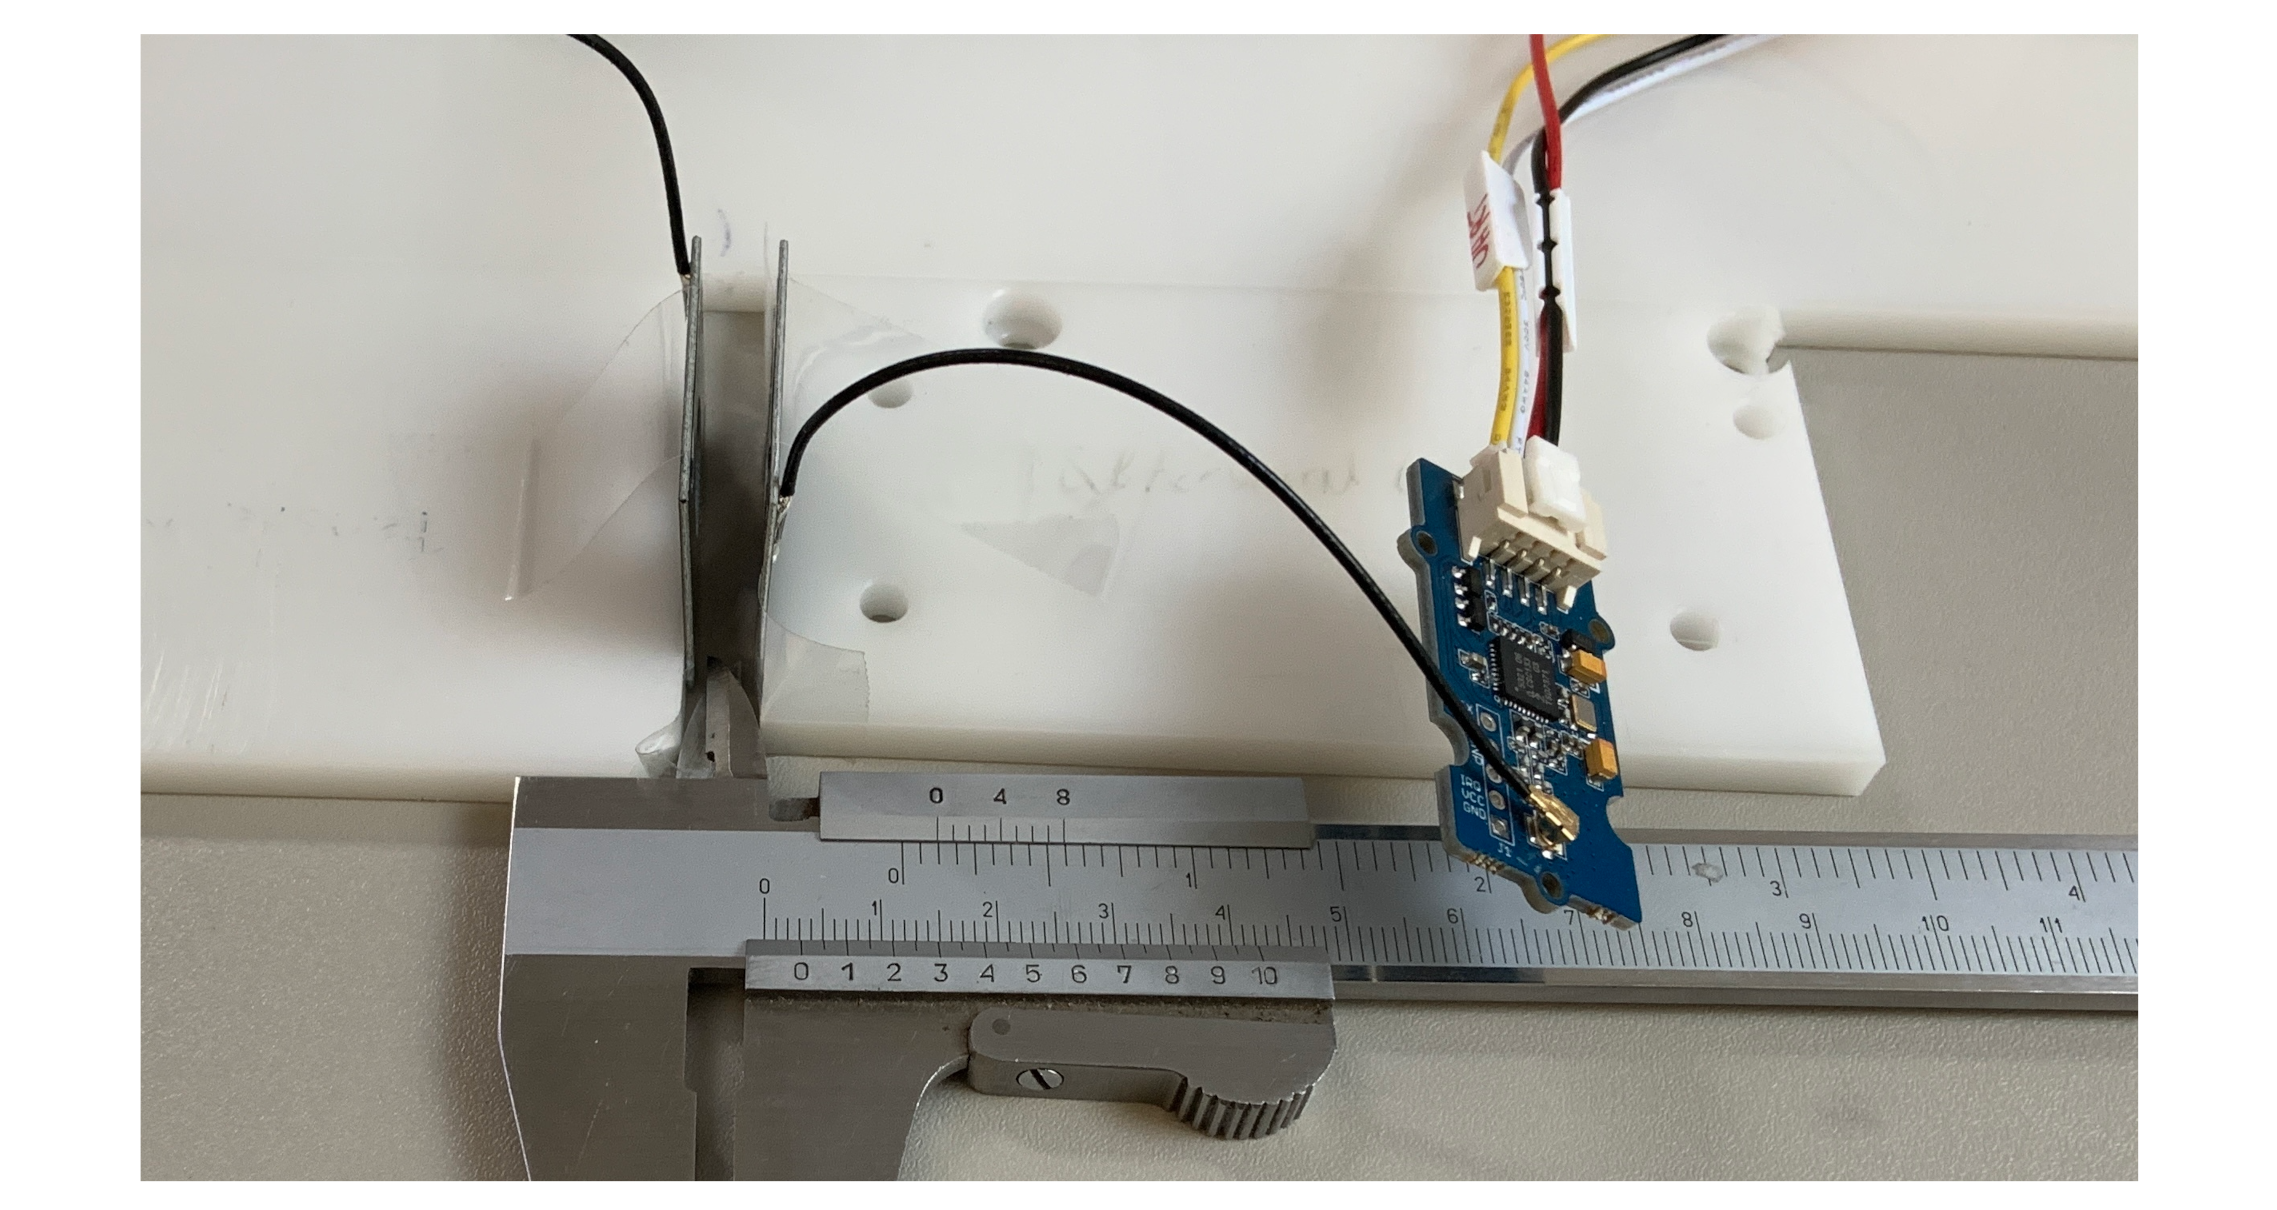
\includegraphics{images/ATC_nfc_range_test.png}
\caption{Grove PN532 NFC Reader mit Kabelgebundener Antenne
\label{ATC_nfc_range_test}}
\end{figure}

Ein Vorteil dieser Technologie ist, dass diese auch im Konsumerbereich
bereits breit verfügbar ist. Durch das einfache Programmieren dieser
\gls{nfc}-Tag über das Smartphone, wird kein zusätzliches
Lese-/Schreib-Gerät benötigt. Hier muss jedoch zuvor getestet werden,
welchen maximalen Abstand nötig ist, um solch ein Tag scannen zu können.
Auch ist der Abstand zwischen den einzelnen Tags entscheidend, wie nah
diese beieinander platziert werden können, um diese einwandfrei auslesen
zu können.

Hierzu wurde ein kleiner Testaufbau \ref{ATC_nfc_range_test} entwickelt,
um verschieden Abstände testen zu können.

Als Lesegerät wurde ein \passthrough{\lstinline!PN532!} Modul zum
Auslesen der \gls{nfc}-Tags eingesetzt, da dieser einfach angesteuert
werden kann und eine abnehmbare Antenne besitzt. Dieser wurde bereits in
anderen Projekten eingesetzt und erwies sich als zuverlässig.

Die im Test verwendeten \gls{nfc}-Tag, haben einen Durchmesser von 22mm
und sind somit ein Standart-Produkt. Im Test stellte sich heraus, dass
diese im gewählten Setup, einen Abstand von 5mm zueinander benötigen.
Der Abstand des Lesegeräts bzw. der Antenne zu einem Tag kann dabei bis
zu 14mm betragen.

Somit eignet sich die Kombination aus Tag und Lesegerät zu einer der
Schachfiguren, wobei sich das Lesegerät unter der Schachtischplatte
befindet.

\hypertarget{schrittmotor-schrittmotorsteuerung}{%
\section{Schrittmotor /
Schrittmotorsteuerung}\label{schrittmotor-schrittmotorsteuerung}}

Da die einzelnen Figuren über das Schachfeld bewegt werden sollen, ist
hierfür eine akkurate Positionierung dieser notwendig. Da die Figuren
einen Durchmesser von 22mm haben und somit ein einzelnes Schachfeld eine
Größe ca. 55mm besitzt, reicht eine Wiederholgenauigkeit von +-1mm. Auch
wird bei der Wahl der passenden Motoren, angenommen dass das Spiel,
welches durch die Mechanik in das System eingebracht wird,
vernachlässigbar klein ist. Es ist auch davon auszugehen, dass die
Kraft, welche von den Motoren benötigt wird, um eine Achse zu bewegen
nicht mehr als 45Ncm beträgt.

Dies entspricht den Werten einer X-Y-Achsenkonfiguration, wie sie in
einem handelsüblichen 3D-Drucker zu finden ist und welche mit
\passthrough{\lstinline!Nema 17!}-Schrittmotoren ausgestattet sind. Der
geplante Aufbau des autonomen Schachtischs, ähnelt einer solchen
Konfiguration sehr, da auch hier die Figuren in X-Y Richtung verfahren
werden. Einzig die Z-Achse kommt hier nicht zum Einsatz. Somit werden
für erste Tests diese Motoren gewählt.

Deswegen bietet sich hier auch die Verwendung von Schrittmotoren an, da
diese sehr kostengünstig in der geforderten Leistungsklasse zu erwerben
sind und zudem kann die Ansteuerung einfach realisiert werden. Hierzu
gibt es verschiedene Schrittmotor-Treiber, welche die Ansteuerung
übernehmen. Diese biete in der Regel ein \passthrough{\lstinline!STEP!},
\passthrough{\lstinline!DIR!} Interface an. Der Schrittmotor-Treiber
besitzt diese beiden Eingänge und jeder Elektrische-Impuls sorgt dafür,
dass der Motor einen Schritt ausführt. Je nach ausgewähltem Motor
entspricht dies einer Rotation um 1.8 Grad und dies reicht somit für die
Positioniergenauigkeit aus.

Da auf dem eingebetteten System auf einem nicht echtzeitfähigen
Linux-System aufsetzt, ist hier eine zeitkritische Ansteuerung der
Motortreiber nicht gewährleistet. Somit stellt sich das
\passthrough{\lstinline!STEP!}, \passthrough{\lstinline!DIR!}-Interface
für diesen Anwendungsfall als nicht ideal heraus. Um dieses Problem zu
umgehen, kann hier ein zusätzlicher Mikrokontroller eingesetzt werden,
welcher die benötigten Impulse generiert.

Diese Option wurde zuvor getestet und erwies sich als eine robuste
alternative, jedoch existieren Schrittmotor-Treiber, welche über
zusätzliche Bus Schnittstellen verfügen. Hier wurde auf den
\passthrough{\lstinline!TMC5160-BOB!} gesetzt, da dieser über eine
\gls{spi} Interface verfügt, welches direkt an das eingebettete System
angeschlossen werden kann.

Somit stellen die Schrittmotoren und die gewählte Ansteuerung einen
vielversprechendes Antriebskonzept für den autonomen Schachtisch dar.

\hypertarget{d-druck-fuxfcr-den-mechanischen-aufbau}{%
\section{3D Druck für den mechanischen
Aufbau}\label{d-druck-fuxfcr-den-mechanischen-aufbau}}

Da es sich hier nur um einen Prototyp handelt, wurde hier auf ein
einfach zu verarbeitendes Filament vom Typ \gls{pla} zurückgegriffen.
Dieses ist besonders gut für die Prototypenendwicklung geeignet und kann
mit nahezu jeden handelsüblichen \gls{fdm} 3D-Drucker verarbeitet
werden.

Zuvor wurden einige Testdrucke durchgeführt, um die Qualität der zuvor
gewählten Druckparameter \ref{3dprintsettings} zu überprüfen und diese
gegebenenfalls anzupassen. Auch wurden verschiedene weitere Bauteile
gedruckt, an welchen die Toleranzen für die späteren \gls{cad}
Zeichnungen abgeschätzt werden können. Dies betrifft vor allem die
Genauigkeit der Bohrungen in den gefertigten Objekten, da hier später
Bolzen und Schrauben ein nahezu spielfrei eingeführt werden müssen. Ein
Test, welcher die Machbarkeit von Gewinden zeigt, wurde nicht
durchgeführt, da alle Schrauben später mit der passenden Mutter
gesichert werden sollen. So soll eine Abnutzung durch häufige Montage
der gedruckten Bauteile verhindert werden.

Bei dem Design der zu druckenden Bauteile wurde darauf geachtet, dass
diese den Bauraum von 200x200x200mm nicht überschreiten und somit auch
von einfachen \gls{fdm} 3D-Druckern erstellt werden können.

Als Software wurde der Open-Source Slicer Ultimaker Cura
\cite{ultimakercura} verwendet, da dieser zum einen bereits fertige
Konfigurationen \ref{3dprintsettings} für den verwendeten 3D-Drucker
enthält und zum anderen experimentelle Features bereitstellt.

\begin{figure}
\centering
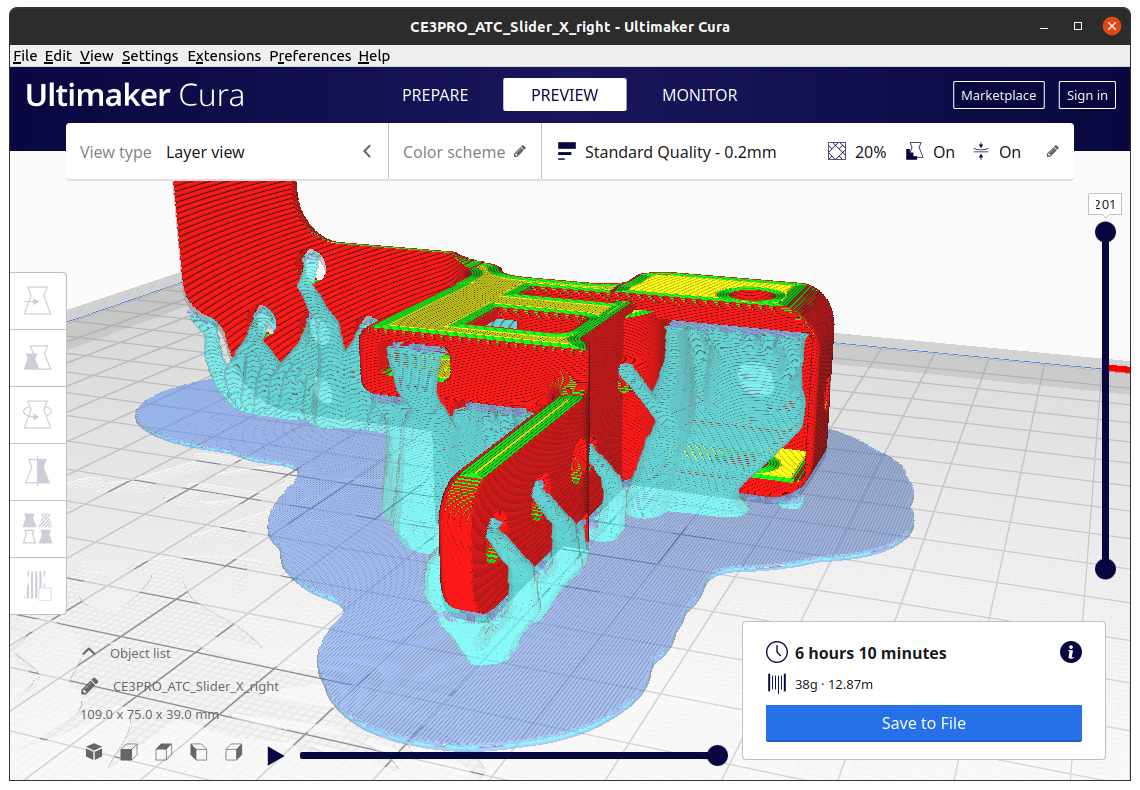
\includegraphics{images/3d_print_tree_structure.png}
\caption{3D Druck: Objekt (rot,gelb,grün),Tree Structure (cyan)
\label{3d_print_tree_structure}}
\end{figure}

Hier wurde für die Bauteile, welche eine Stützstruktur benötigen, die
von Cura bereitgestellte Tree Support Structure aktiviert.
\ref{3d_print_tree_structure} Diese bietet den Vorteil gegenüber anderen
Stützstrukturen, dass sich diese leichter entfernen lässt und weniger
Rückstände an den Bauteilen hinterlässt. Diese Vorteile wurde mit
verschiedenen Testdrucken verifiziert und kommen insbesondere bei
komplexen Bauteilen mit innenliegenden Elementen zum Tragen, bei denen
eine Stützstruktur erforderlich sind.

\begin{longtable}[]{@{}lr@{}}
\caption{Verwendete 3D Druck Parameter. Temperatur nach
Herstellerangaben des verwendeten PLA Filament.
\label{3dprintsettings}}\tabularnewline
\toprule
Ender 3 Pro 0.4mm Nozzle & PLA Settings\tabularnewline
\midrule
\endfirsthead
\toprule
Ender 3 Pro 0.4mm Nozzle & PLA Settings\tabularnewline
\midrule
\endhead
Layer Height & 0.2mm\tabularnewline
Infill & 50.00\%\tabularnewline
Wall Thickness & 2.0mm\tabularnewline
Support Structure & Tree\tabularnewline
Top Layers & 4\tabularnewline
Bottom Layers & 4\tabularnewline
\bottomrule
\end{longtable}

Zusätzliche Parameter wie die Druckgeschwindigkeit, sind hierbei
individuell für den zu gewählten 3D Drucker zu ermitteln. Allgemein
wurden hier die Standarteinstellungen verwendet, welche in diesem Falle
einen guten Kompromiss zwischen Qualität und Druckzeit lieferten.

\hypertarget{erstellung-erster-prototyp}{%
\chapter{Erstellung erster Prototyp}\label{erstellung-erster-prototyp}}

\begin{figure}
\centering
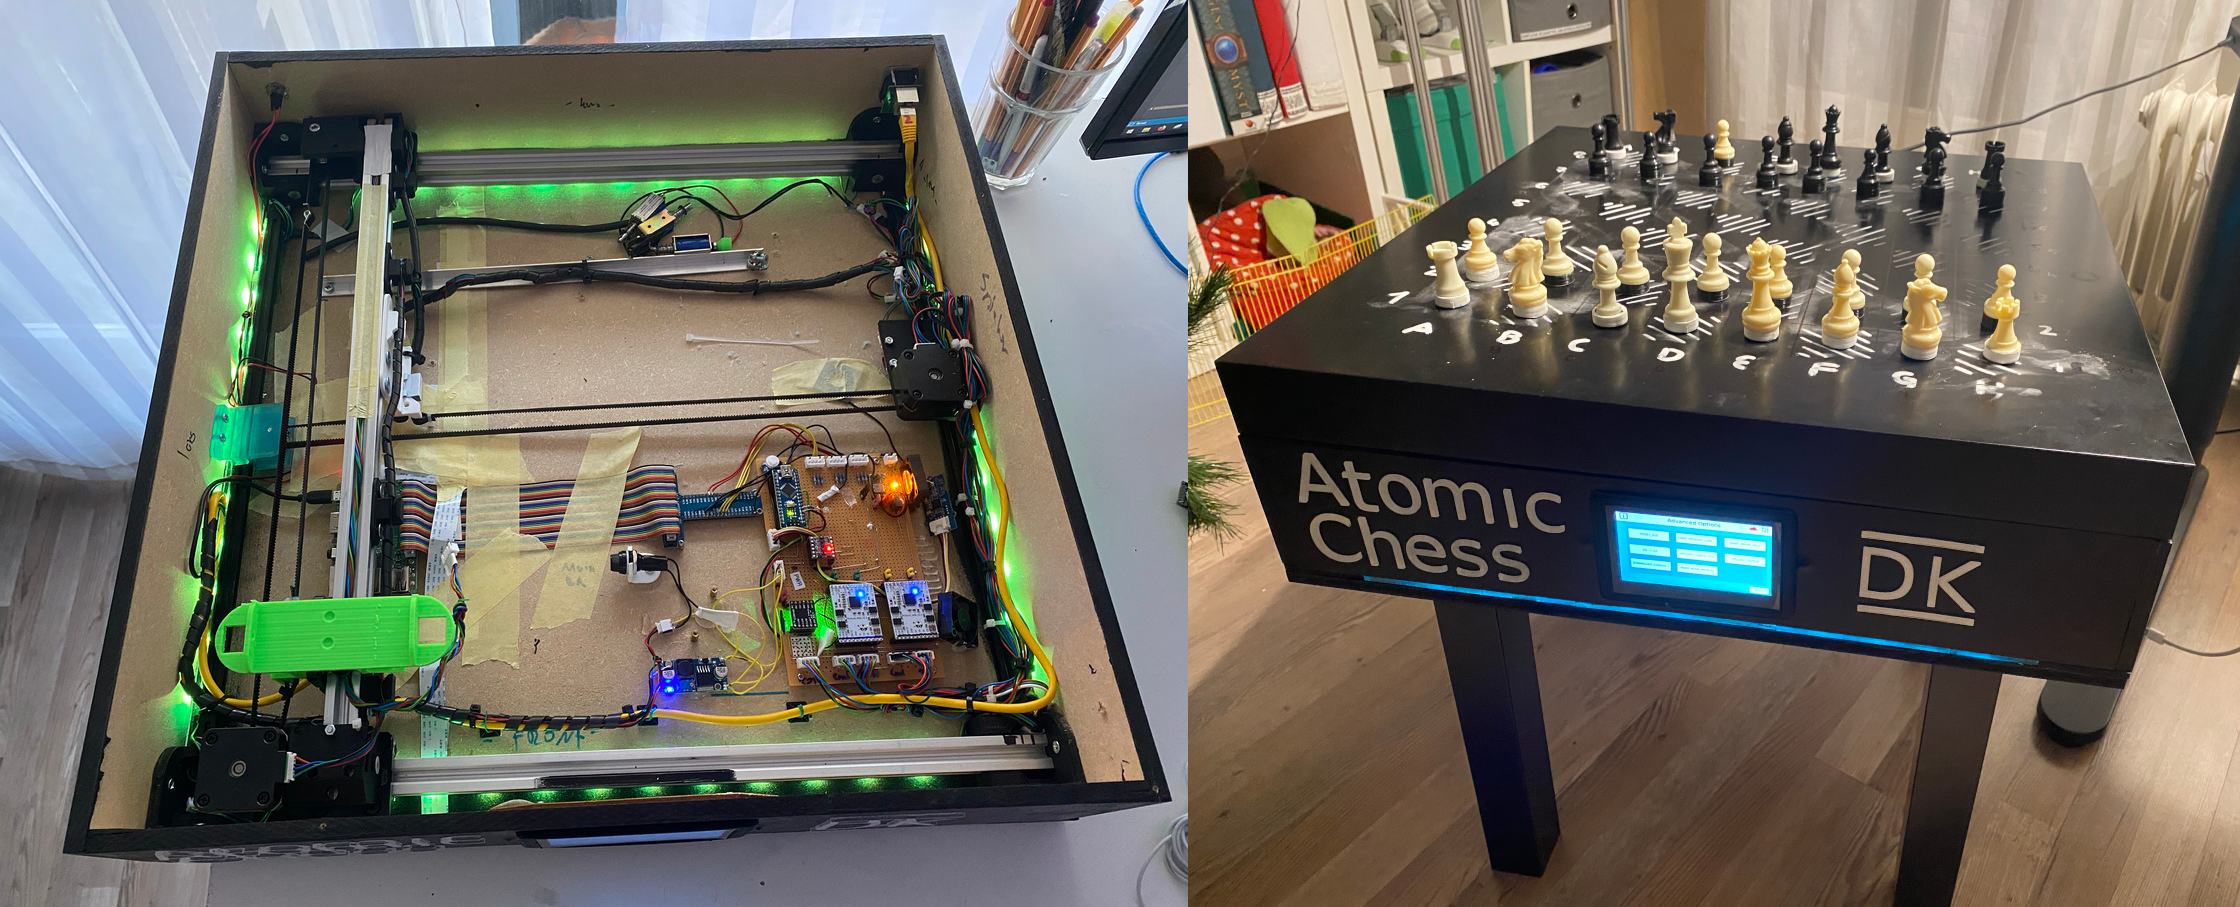
\includegraphics{images/table_images/dk.png}
\caption{Prototyp Hardware: Erster Prototyp des autonomen Schachtisch
\label{dk}}
\end{figure}

\hypertarget{mechanik}{%
\section{Mechanik}\label{mechanik}}

Bei dem mechanischen Aufbau wurde auf ein einfaches Design geachtet. Die
Konstruktion wurde im Vorfeld in einem \gls{cad} Programm durchgeführt
und die Grundkonstruktion in mehreren Iterationsschritten verfeinert.
Das verwendete \gls{cad} Programm
\passthrough{\lstinline!Autodesk Fusion 360!} bietet, eine einfache
Umsetzung auch für Personen, welche keine Ausbildung im Bereich der
Mechanik und Entwicklung vorweisen können.

Bei der initialen Planung wurde beachtet, einen möglichst kleinen
Fußabdruck des Schachtischs zu realisieren. Darüber hinaus wurde
beabsichtigt, eine fertige Schachtischplatte als Basis zu verwenden und
die Mechanik unter diese zu konstruieren. Um dies zu ermöglichen wurde
ein IKEA Lack Tisch verwendet, welcher die Idealen Abmessungen von
55x55cm hat und somit eine erforderliche Schachfeldgröße von 55mm
möglich ist. Durch den bereits vorhandenen Rahmen ist es simpel möglich,
weitere Komponenten an diesem zu befestigen. Somit stellt diese
Tischplatte eine ideale Basis für den autonomen Schachtisch dar.

Für die Achsenführung der beiden X- und Y-Achsen wurden konventionelle
20x20mm V-Slot Aluminium-Profile verwendet, welche mit einfachen Mitteln
und wenig Geschick passend zugeschnitten werden können. Allgemein wurde
eine X-Y Riemenführung verwendet, wobei jede Achse einen separaten Nema
17 Schrittmotor inklusive des passenden Endschalters montiert hatte. Bei
den Schlitten, welche auf den Aluminium-Profilen laufen, wurden fertige
Standartkomponenten verwendet, um das Spiel in der Mechanik zu
minimieren. Diese stellen jedoch einen großen Posten in der
Preiskalkulation dar. Die Vorteile überwogen jedoch, da diese nicht
manuell erstellt und getestet werden müssen.

Bereits während des Designprozess konnte anhand einer statischen
Simulation des Modells erkannt werden, dass trotz der Optimierung des
Fahrweges beider Achsen durch die Verkleinerung der Halterungen der
Aluminium-Profile dieser nicht ausreicht. Mit dieser Konstellation
können die Figuren nicht ausreichend weit aus dem Spielfeld platziert
werden und verbleiben in den äußeren Spielfeldern. Dieser Effekt war
unerwünscht und schränkt das Spielerlebnis deutlich ein.

\begin{figure}
\centering
\includegraphics{images/ATC_DK_HW_DUAL_COIL.png}
\caption{Zwei Elektromagnete. Schlitten befindet sich jeweils in den
Ecken \label{ATC_DK_HW_DUAL_COIL}}
\end{figure}

Um dies zu verhindern wurde der zentrale Schlitten der Y-Achse, auf
welchem der Elektromagnet für die Figur-Mitnahme platziert ist, um einen
weiteren Elektromagnet erweitert. Diese befinden sich nun nicht mehr
mittig auf dem Schlitten, sondern wurden um 110mm in Richtung der
X-Achse versetzt \ref{ATC_DK_HW_DUAL_COIL}. So ist es möglich Figuren
bis ganz an den Rand verschieben zu können.

Diese Lösung erfordert jedoch einen komplexeren
Bahnplanungs-Algorithmus, da die Elektromagneten zwischen einzelnen
Zügen gewechselt werden müssen. Dies führt zu einem zeitlich kürzeren
Stillstand der Figur auf dem Schachfeld.

Alle selbst-konstruierten Teile wurden anschließend mittels 3D Druck
erstellt und konnten in die Tischplattenbasis eingeschraubt werden. Die
Verwendung der aus Holz bestehenden Grundplatte erschwerte jedoch eine
akkurate Platzierung der Teile und die bereits existierenden Seitenwände
schränkten diese noch zusätzlich ein. Somit erforderte der komplette
Zusammenbau mehrere Tage und zusätzliche Iterationen des 3D-Designs, um
den Einbau spezifischer Teile zu ermöglichen. Das Design stellt jedoch
eine solide Grundlage darf, welche für die weitere Software und
Hardware-Entwicklung essentiell ist.

\hypertarget{parametrisierung-schachfiguren}{%
\section{Parametrisierung
Schachfiguren}\label{parametrisierung-schachfiguren}}

Da das System die auf dem Feld befindlichen Schachfiguren anhand von
\gls{nfc} Tags erkennt, müssen diese zuerst mit Daten beschrieben
werden. Die verwendeten NXP
\passthrough{\lstinline!NTAG 21!}\cite{nxpntag21} \gls{ic}, besitzen
einen vom Benutzer verwendbaren Speicher von 180 Byte. Dieser kann über
ein \gls{nfc}-Lese/Schreibger mit Daten verschiedenster Art beschrieben
und wieder ausgelesen werden. Moderne Mobiltelefone besitzen in der
Regel auch die Fähigkeit mit passenden \gls{nfc} Tags kommunizieren zu
können; somit sind keine Stand-Alone Lesegeräte mehr notwendig.

Der Schachtisch verwendet dabei das \gls{ndef} Dateiformat welches
Festlegt, wie die Daten auf dem \gls{nfc} Tag gespeichert werden. Da
diesen ein Standardisiertes Format ist, können alle gängigen Lesegeräte
und Chipsätze diese Datensätze lesen. Der im autonomen Schachtisch
verwendete Chipsatz \passthrough{\lstinline!PN532!} von NXP ist dazu
ebenfalls in der Lage.

Um das \gls{ndef} Format verwenden zu können, müssen die \gls{nfc} Tags
zuerst auf diese formatiert werden. Die meisten käuflichen Tags sind
bereits derart formatiert. Alternativ kann dies mittels Mobiltelefon und
passender Applikation geschehen. Da \gls{ndef} Informationen über die
Formatierung und der gespeicherten Einträge speichert, stehen nach der
Formatierung nur noch 137 Bytes des NXP NTAG 21 zur Verfügung.

Per Lesegerät können anschließend mehrere \gls{ndef} Records auf den Tag
geschrieben werden. Diese sind mit Dateien auf einer Festplatte
vergleichbar und können verschiedenen Dateiformate und Dateigrößen
annehmen. Ein typischer Anwendungsfall ist der \gls{ndefrtd} URL
Datensatz. Dieser kann dazu genutzt werden eine spezifizierte URL auf
dem Endgeräte aufzurufen, nachdem der \gls{nfc} Tag gescannt wurde.
\cite{nordicnfclibndef}

Der autonome Schachtisch verwendet den einfachsten \gls{ndefrtd} Typ,
den sogenannten Text-Record, welcher zum Speichern von Zeichenketten
genutzt werden kann, ohne das eine Aktion auf dem Endgerät ausgeführt
wird. Jeder Tag einer Schachfigur, welche für den autonomen Schachtisch
verwendet werden kann, besitzt diesen \gls{ndef} Record
\ref{ndef_record_rook} an der ersten Speicher-Position. Alle weiteren
eventuell vorhandenen Records werden vom Tisch ignoriert.
\cite{nordicnfclib}

\begin{figure}
\centering
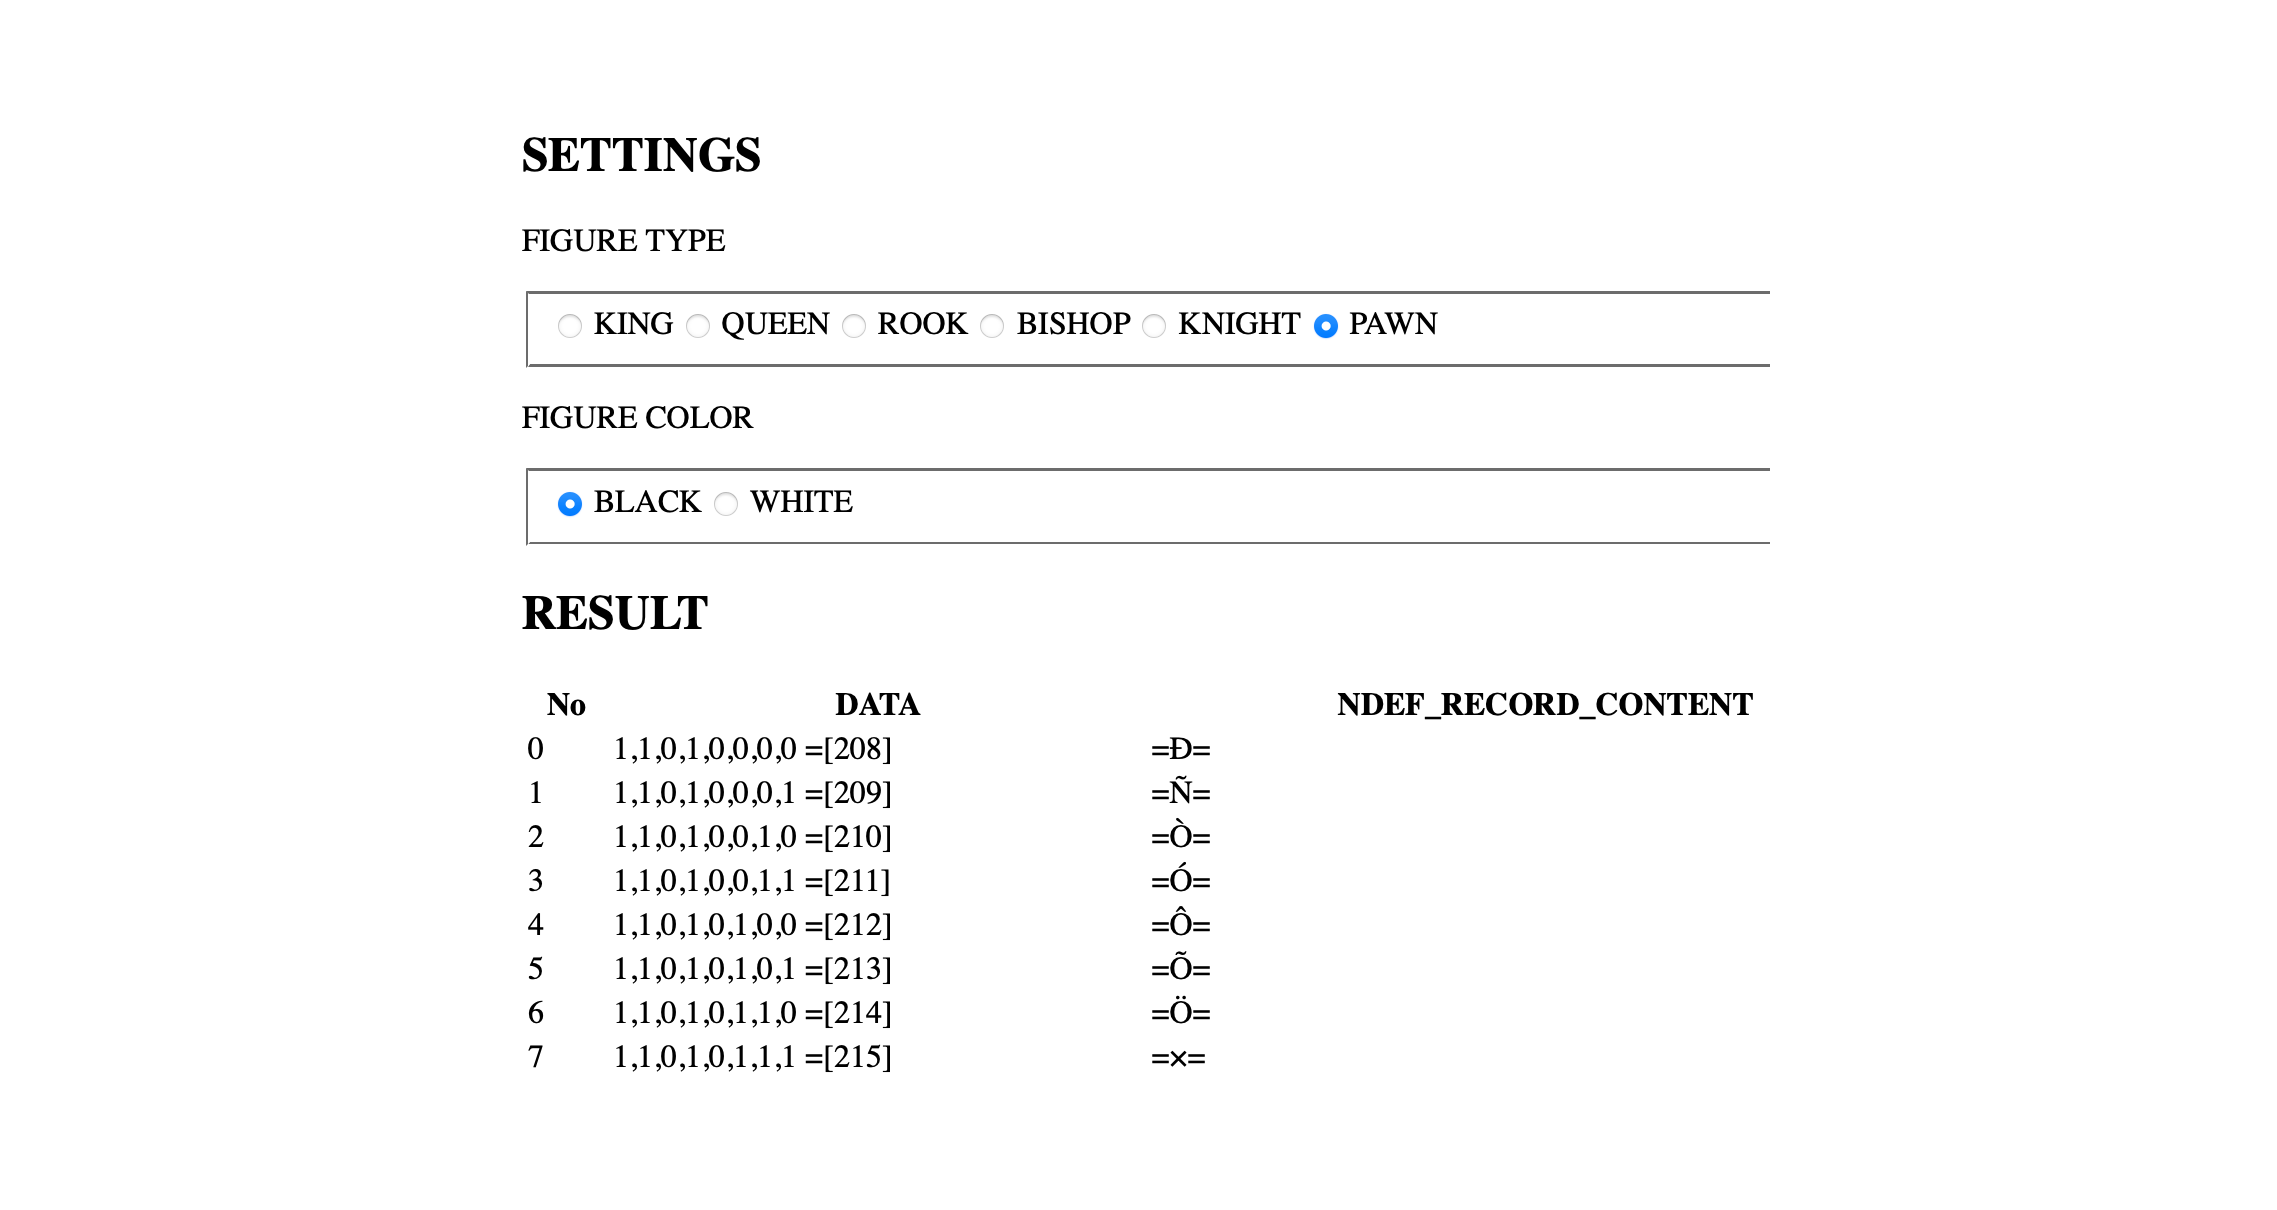
\includegraphics{images/ATC_ChessFigureIDGenerator.png}
\caption{Prototyp Hardware: Tool zur Erstellung des NDEF Payloads:
ChessFigureIDGenerator.html \label{ATC_ChessFigureIDGenerator}}
\end{figure}

Um die Payload für den \gls{nfc} Record zu erstellen wurde ein kleine
Web-Applikation \ref{ATC_ChessFigureIDGenerator} erstellt, welche den
Inhalt der Text-Records erstellt. Dieser ist für jede Figur individuell
und enthält den Figur-Typ und die Figur-Farbe. Das Tool unterstützt auch
das Speichern weiterer Attribute wie einem Figur-Index, welcher aber in
der finalen Software-Version nicht genutzt wird.

\begin{figure}
\centering
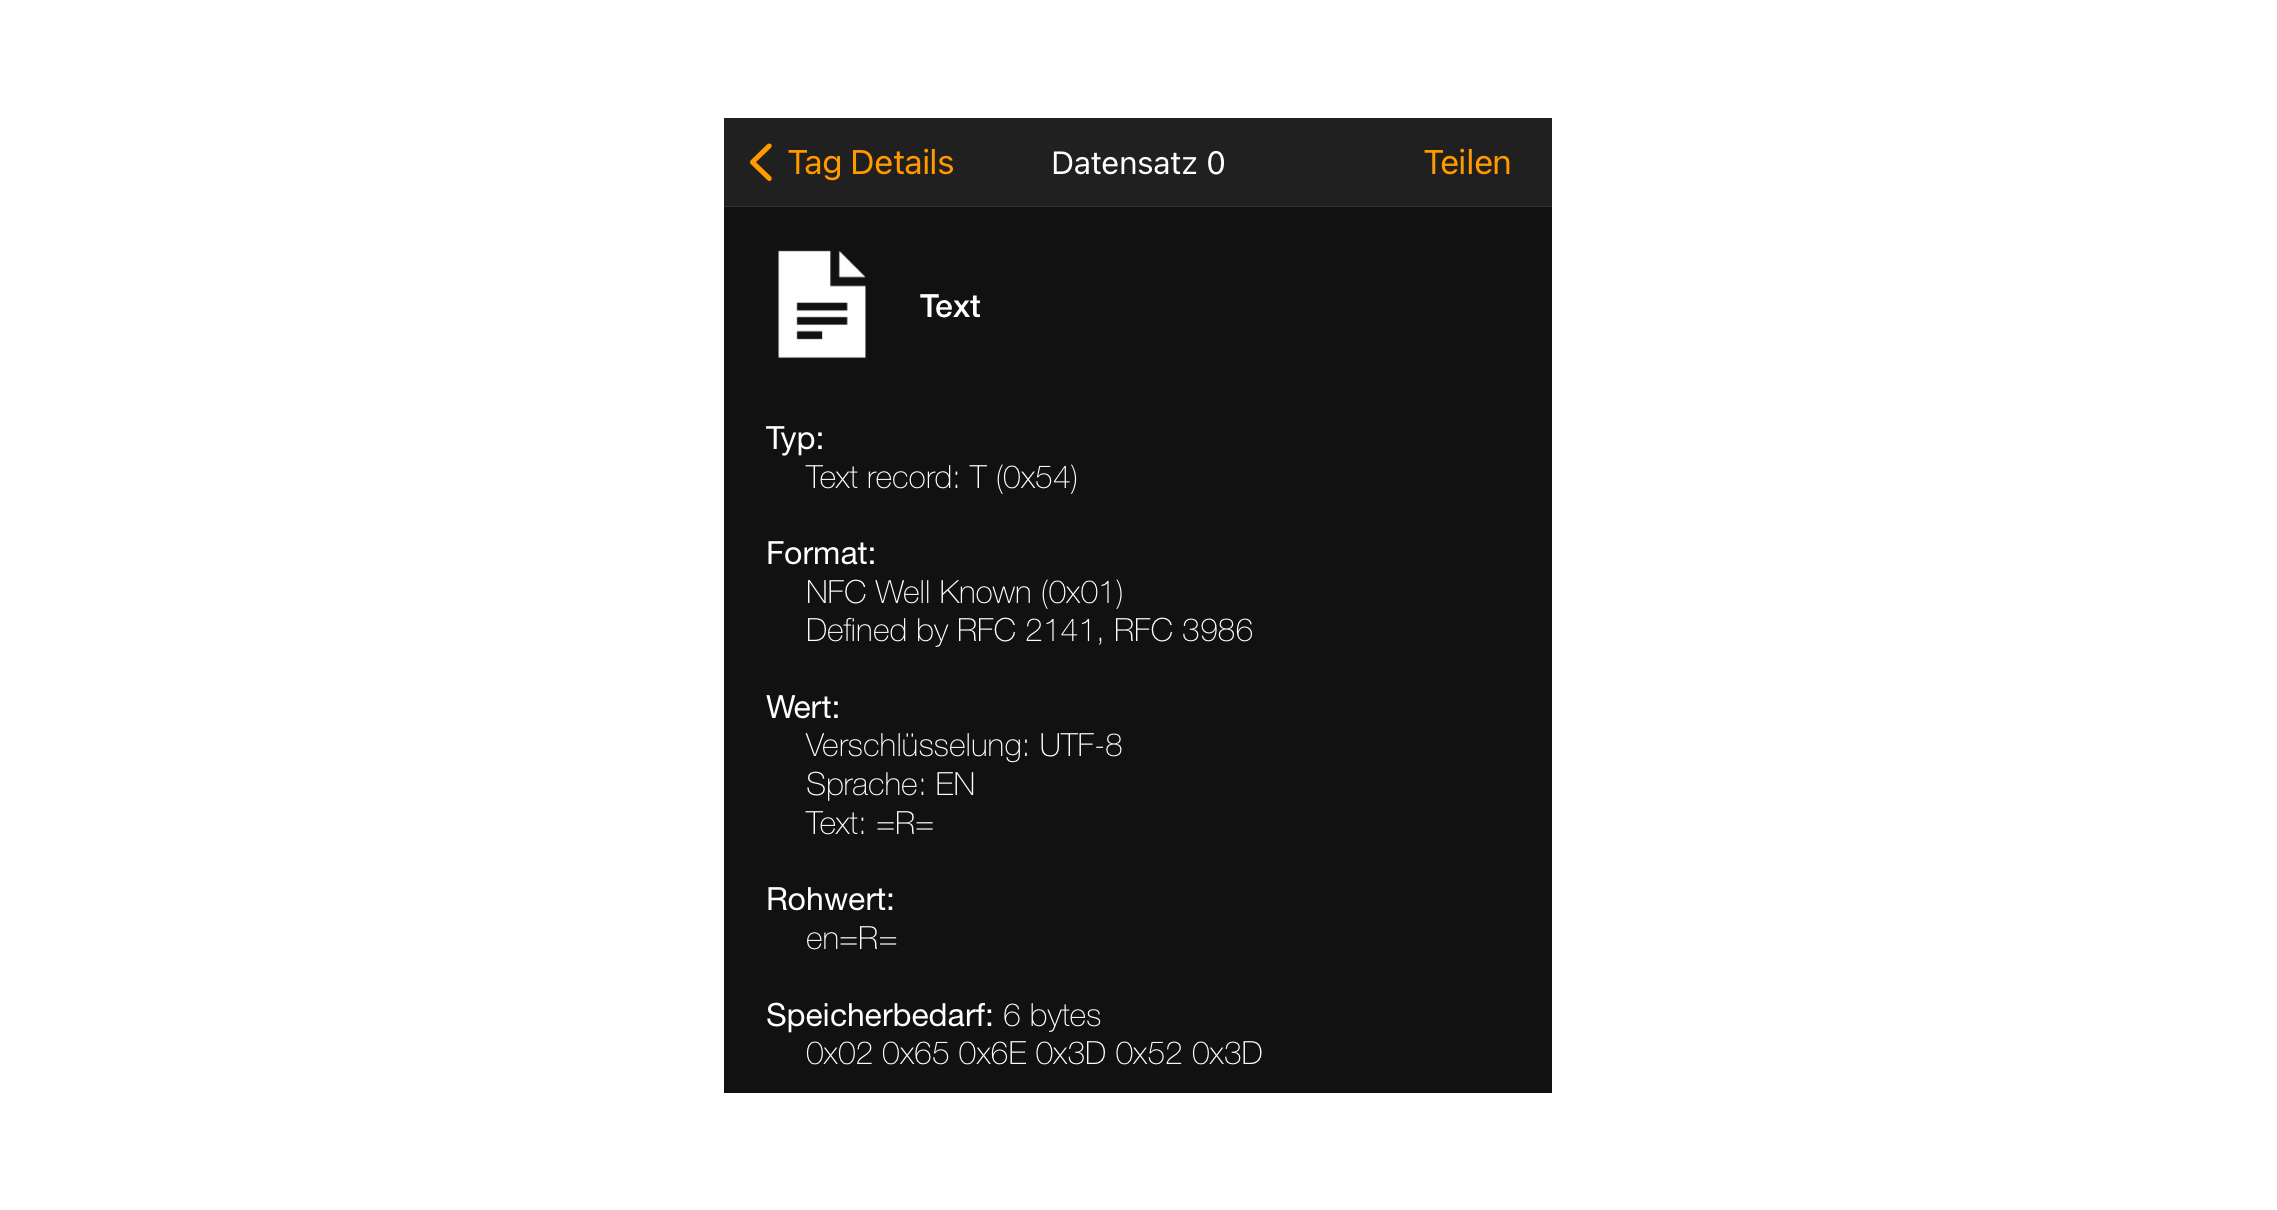
\includegraphics{images/ndef_record_rook.png}
\caption{Prototyp Hardware: NDEF Text Record Payload für einen weißen
Turm \label{ndef_record_rook}}
\end{figure}

Nach dem Beschreiben eines \gls{nfc} Tags ist es zusätzlich möglich,
diesen gegen Auslesen mittels einer Read/Write-Protection zu schützen.
Diese Funktionalität wird jedoch nicht verwendet, um das Kopieren
einzelner Figuren durch den Benutzer zu ermöglichen. Somit kann dieser
leicht seine eigenen Figuren erschaffen, ohne auf das Tool angewiesen zu
sein. Auch ist es so möglich, verschiedene Figur-Sets zu mischen; somit
kann ein Spieler verschiedene Sets an Figuren mit dem autonomen
Schachtisch verwenden.

\hypertarget{schaltungsentwurf}{%
\section{Schaltungsentwurf}\label{schaltungsentwurf}}

\begin{figure}
\centering
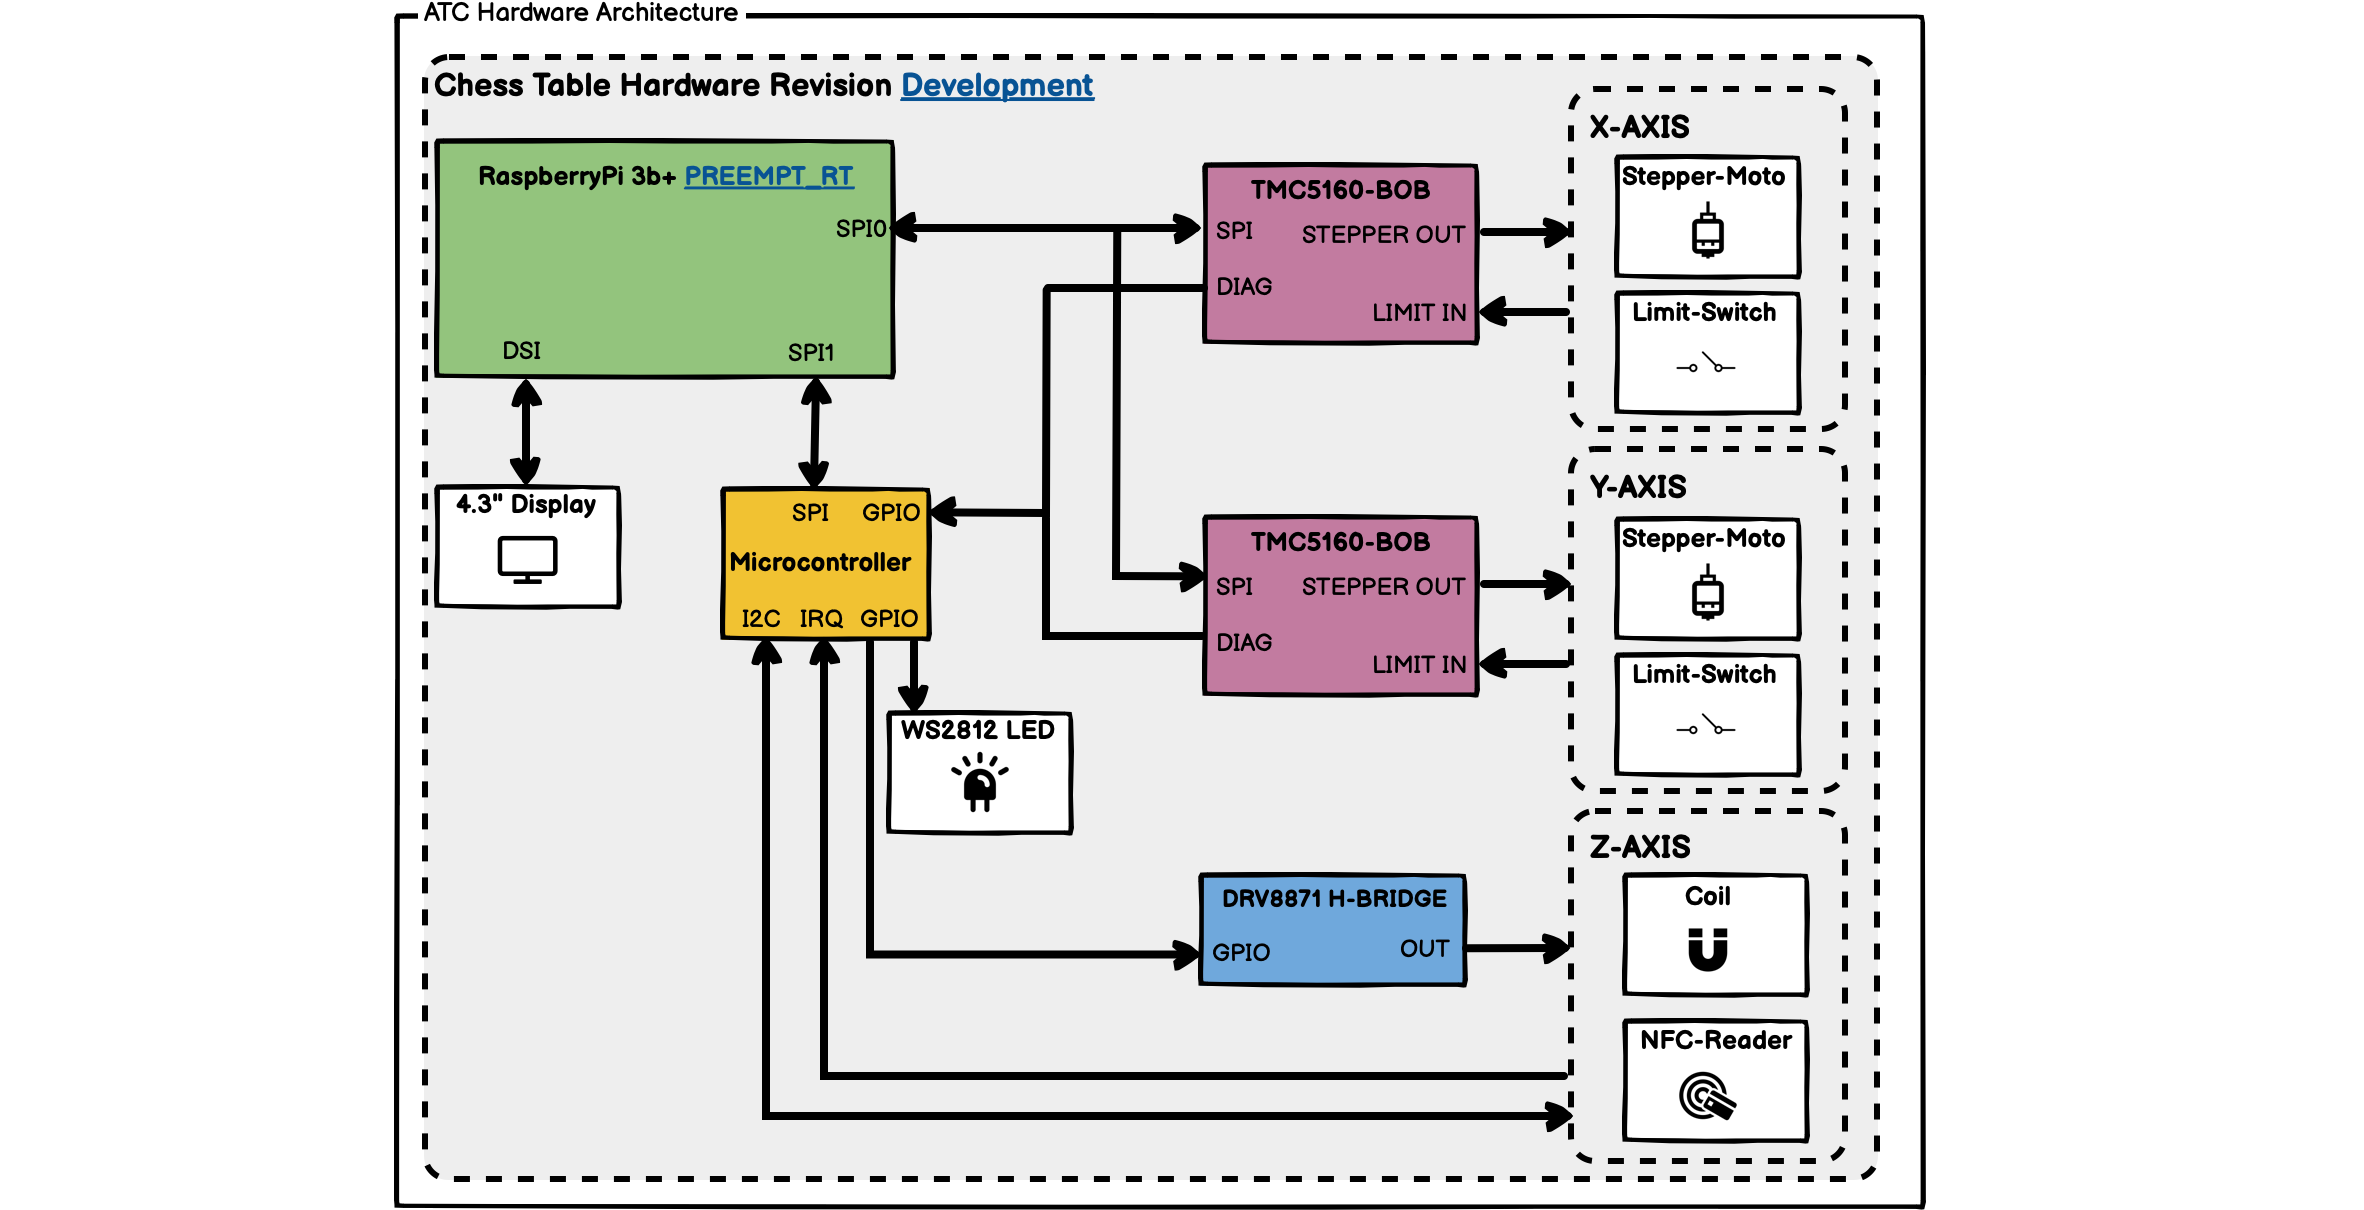
\includegraphics{images/ATC_Hardware_Architecture_DK.png}
\caption{Prototyp Hardware: Blockdiagramm
\label{ATC_Hardware_Architecture_DK}}
\end{figure}

Durch die zuvor durchgeführte Validierung der verwendeten Technologien,
konnte ein Blockdiagramm \ref{ATC_Hardware_Architecture_DK} der
verwendeten elektrischen Komponenten angefertigt werden. Dieses enthält
zum einen die zwei Schrittmotor-Treiber und zum anderen die Komponenten
zur Ansteuerung der beiden Elektromagnete sowie das
\passthrough{\lstinline!PN532!} Module zum Auslesen der \gls{nfc} Tags.

Die wichtigsten Komponenten in der Schaltung sind das eingebettete
System und die beiden Schrittmotortreiber
\passthrough{\lstinline!TMC5160-BOB!}. Diese sind direkt über einen
\gls{spi} Bus miteinander verbunden. Zusätzlich zu den Schrittmotoren
selbst, ist an jedem Treiber der Endschalter zur Durchführung der
Referenzfahrt der Achse angeschlossen. Die Treiber bieten dabei Eingänge
für zwei Endschalter, jeodch wird nur ein Endschalter für die minimale
Position (Home Position) benötigt. Die Treiber sind direkt mit der
Eingangsspannung verbunden, werden jedoch durch eine 5A Glassicherung
geschützt. Da der \gls{spi} Bus und die Treiber mit dem 3.3V Logikpegel
des eingebetteten Systems kompatibel sind, können diese direkt
miteinander verbunden werden. Dieser Bus ist in einer
Stern-Konfiguration aufgebaut, was zur Folge hat, dass jeder Treiber ein
zusätzliches Chip-Select Signal benötigt. Diese wurden ebenfalls mit dem
eingebetteten System verbunden.

Zusätzlich sind Spannungswandler nötig, um die erforderlichen Spannungen
von 12V für die Elektromagnete und 5V für das eingebettete System zu
erzeugen. Die Schrittmotoren werden direkt mit der Versorgungsspannung
von 14-24V betrieben. Alle weiteren verwendeten Komponenten zu denen
unter anderem auch das \passthrough{\lstinline!PN532!} \gls{nfc} Modul
und die \passthrough{\lstinline!WS2811!} \gls{led} Module gehören,
werden ebenfalls über die 5V Schiene versorgt.

Für den Betrieb der beiden Elektromagnete wurde kein N-Channel Mosfet
o.ä. verwendet, da hier auf maximale Flexibilität der Ansteuerung
ausschlaggebend ist und bisher nicht ausreichend Erfahrung mit dem
Verhalten dieser im Zusammenspiel mit den magnetischen Schachfiguren
gesammelt werden konnte. Deshalb wurde hier eine H-Brücke
\passthrough{\lstinline!DRV8871H!} verwendet, somit kann auch die
Polarität im Nachhinein per Software geändert werden und nicht nur die
Spannung über ein \gls{pwm} Signal. Der verwendete Treiber besitz
darüber hinaus zwei Ausgänge, was den Nutzen dieser Module besonders
ausweitet.

Für die Erzeugung der \gls{pwm} Signale für die H-Brücke wurde ein
zusätzlicher Mikrokontroller \passthrough{\lstinline!Atmega328p!}
benötigt, da hier die Steuersignale nicht direkt vom eingebetteten
System erzeugt werden, sondern nur die Zustandsinformationen über den
\gls{spi} Bus übertragen werden sollen. Dies spart zusätzliche
\gls{gpio} Anschlüsse und somit sind alle Kompomenten über einen
zentralen Bus kontrollierbar, welches einen möglichen Tausch des
eingebetteten Systems in späteren Revisionen vereinfacht.

Der zusätzliche Mikrokontroller übernimmt auch die Kommunikation mit dem
\passthrough{\lstinline!PN532!} Modul, da dieses sonst über seine
\gls{i2c} Schnittstelle mit einem entsprechenden Host-System
kommuniziert. Der Mikrokontroller übernimmt somit ebenfalls die
Konversation des \gls{i2c} Bus hin zum zentralen \gls{spi} Bus. Zu
beachten ist, dass nun ein zusätzlicher Chip-Select \gls{gpio} zum
Ansteuern der Elektromagnete und des \passthrough{\lstinline!PN532!}
Moduls benötigt wird. Dies wird durch die Firmware, welche auf dem
Mikrokontroller ausgeführt wird, realisiert, und je nach empfangenem
Kommando die entsprechende Komponente ausgewählt.

\begin{figure}
\centering
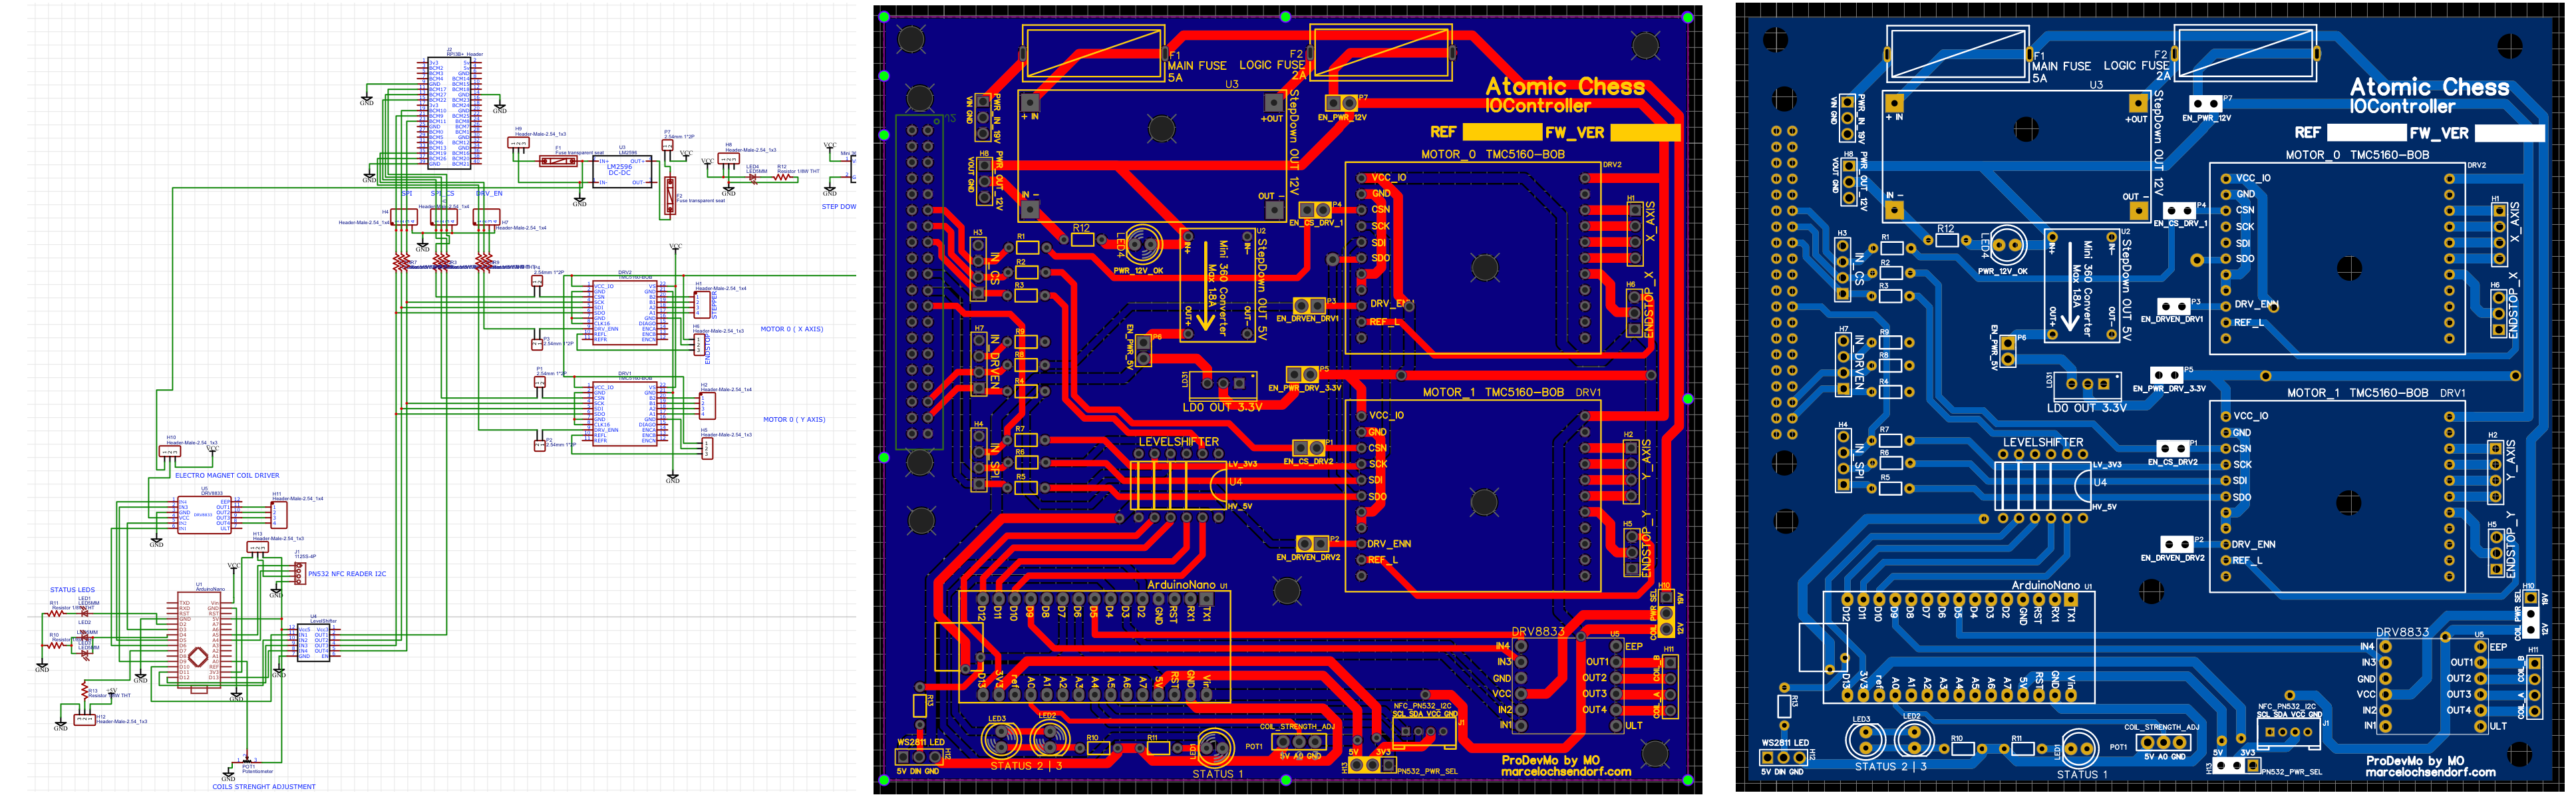
\includegraphics{images/ATC_DK_HW_SCHEM.png}
\caption{Prototyp Hardware: Schaltplan und finaler PCB Entwurf
\label{ATC_Schematic_DK}}
\end{figure}

Nach der Festlegung der zu verwendenden Komponenten, wurde ein
entsprechender Schaltplan \ref{ATC_Schematic_DK} nach den zuvor
erörterten Vorgaben entworfen. Hierbei wurde die Vorgaben der
Datenblätter und der Application-Notes in diesen Orientiert. Da es sich
hier um einen ersten Funktionsentwurf handelt, wurde zusätzliche
Testpunkte in das Design eingefügt.

Somit ist es während der weiteren Entwicklung möglich, zusätzliches
Testequipment wie einen Logic-Analyser direkt an den \gls{spi} Bus oder
ein Oszilloskop an die Ausgänge der H-Brücke dauerhaft anzuschliessen.
Desweiteren ist es mögliche die Bus- und Spannungsversorgung über Jumper
zu trennen, um einen Funktionstest einzelner Komponenten durchführen zu
können.

Allgemein verwenden alle Komponenten, 3.3V als Logik-Pegel. Trotzdem
wurde ein Levelshifter eingesetzt, welcher den \gls{spi} Bus des
eingebetteten Systems mit dem der Mikrokontroller trennt.

Durchgeführte Tests mit dem verwendeten
\passthrough{\lstinline!Atmega328p!} haben ergeben, dass dieser nicht
direkt mit 3.3V und einer Taktfrequenz von 16MHz betrieben werden kann
und es somit zu einem nicht kontrollierbaren Verhalten dieses kommt.
Dieses Verhalten machten sich durch eine gestörte Kommunikation mit dem
\passthrough{\lstinline!PN532!} Modul bemerkbar und eine Auslesen von
\gls{nfc} Tags war nur in 60\% der Fälle fehlerfrei möglich.

Im Anschluss wurde die Versorgungsspannung auf 5V erhöht, welches zur
Folge hat, dass die Ein- und Ausgänge ebenfalls mit diesem Pegel
arbeiten; dieser Schritt wurde zum Schutz des eingebetteten Systems und
dessen \gls{gpio} Schnittstelle notwendig.

\begin{figure}
\centering
\includegraphics{images/ATC_DK_HW_LOCHRASTER.png}
\caption{Prototyp Hardware: Aufbau der Lochrasterplatine
\label{ATC_DK_HW_LOCHRASTER}}
\end{figure}

Der Schalplan und dessen Funktionalität, wurden anschließend durch den
Aufbau der vollständigen Schaltung auf einer Lochrasterplatine
\ref{ATC_DK_HW_LOCHRASTER} im Eurokartenformat manuell aufgebaut und
getestet.

Aus diesem Design wurde ein \gls{pcb} Layout für eine einfache 2 lagige
Platine erstellt. Dieses orientiert sich an der zuvor umgesetzten
Lochrasterplatine und spiegelt das Layout wider. Auch wurde hier nicht
auf den Platzverbrauch geachtet. Es wurde zusätzliche Steckverbindungen
für die externen Komponenten eingefügt und passende Bohrungen an den
Ecken sowie in der Mitte zur Montage vorgesehen. Auf dem obersten Layer
wurde der Bestückungsdruck erhöht und mit zusätzlicher Information über
die Pin-Belegungen der einzelnen Stecker erweitert.

\hypertarget{implementierung-hal}{%
\section{Implementierung HAL}\label{implementierung-hal}}

Die \gls{hal} stellt das Verbindungsglied zwischen der Hardware und der
Benutzer-Software dar. In diesem Fall übernimmt diese die Übersetzung
der Befehle der Controller-Software in für die Hardware verständliche
Befehle. Dabei geschieht dies über den zentralen \gls{spi} Bus, welcher
im Linux-System als Datei unter dem Pfad
\passthrough{\lstinline!/dev/spidev0.0!} eingebunden wird und über
Dateioperation (lesen, schreiben) mittels
\passthrough{\lstinline!ioctl!} konfiguriert werden kann. Weiterhin
können Daten über das File-Handle gelesen- und geschrieben werden. Somit
ist eine Kommunikation mit der Hardware-Ebene möglich.

Diese Funktionalität wird von der für diese Projekte implementierten
\gls{hal} in Form einer C++ Klasse abgebildet und ermöglicht einen
einfachen Zugriff auf die elektrisch verbundenen Komponenten. Zusätzlich
wird in dieser auch das Hardware-Versions-Management abgebildet. Da im
Verlauf der Entwicklung mehrere Hardware-Revisionen gebaut wurden und
die Controller-Software weiterhin mit allen Revisionen kompatibel sein
soll, ermittelt die \gls{hal} vor dem Start die entsprechende Revision.
Dazu wird die Prozessor-\gls{id} (welche mittels des
\passthrough{\lstinline!cat /proc/cpuinfo | grep Serial | cut -d ' ' -f 2!}
Kommandos abgefragt werden kann) des Systems abgefragt und mittels einer
statischen Liste diese ermittelt. Hierbei enthält die Tabelle nur
Revisionsinformationen über die während der Entwicklung entstandenen
Revisionen. Sollte die Prozessor-\gls{id} nicht hinterlegt sein, geht
das System von der aktuellen Revision aus, so ist keine manuelle Pflege
der Tabelle während einer möglichen Produktion nötig.

\begin{lstlisting}[language={C++}]
//HardwareInterface.h
//...
class HardwareInterface
{
  enum HI_HARDWARE_REVISION {
        HI_HWREV_UNKNOWN = 0,
        HI_HWREV_DK   = 1, //FIRST 55x55cm ATC TABLE WITH TWO COILS
        HI_HWREV_PROD = 2, //SECONDS GENERATION BASED ON SKR1.3 3D PRINT CONTROLLER
        HI_HWREV_PROD_V2 =3,  //THIRD GENERATION WITH SKR 1.4 WITH CORE XY MECHANIC
        HI_HWREV_VIRT=4, //SIMULATED HW FOR TESTING USING THE DOCKERFILE
    };

  enum HI_COIL
    {
        HI_COIL_A   = 0,
        HI_COIL_B   = 1,
        HI_COIL_NFC = 2
    };
  //....
  //MOTOR CONTROL FUNCTIONS
  void enable_motors();
  void disable_motors();
  bool is_target_position_reached();
  void move_to_postion_mm_absolute(const int _x, const int _y, const bool _blocking);
  void home_sync();
  //...
  //LED CONTROL FUNCTIONS
  bool setTurnStateLight(const HI_TURN_STATE_LIGHT _state);
  //NFC CONTROL FUNCTIONS
  ChessPiece::FIGURE ScanNFC();
  //MAGNET CONTROL FUNCTIONS
  bool setCoilState(const HI_COIL _coil, const bool _state);
  //...
\end{lstlisting}

Je nach ermittelter Revision werden die erforderlichen
Hardwarekomponenten initialisiert. Bei allen über den \gls{spi} Bus
angeschlossenen Komponenten, werden nach der Initialisierung des
\gls{spi} Bus auf der Betriebssystem-Ebene, zusätzliche Versionsregister
der einzelnen Komponenten abgefragt. Dies stellt sicher, dass alle
Komponenten mit dem System verbunden sind. Allgemein kann eine
Datentransfer über den \gls{spi} drei Mal fehlschlagen bevor die
Software mittels eines Fehlers abbricht. Gerade bei der Kommunikation
mit dem Mikrokontroller, kam es bei Testläufen zu Fehlern bezüglich der
\gls{spi} Kommunikation, sofern das \gls{nfc}-Modul aktiv war. Um ein
direktes Beenden der Software zu verhindern, wurde diese Art der
Fehlerbehandlung eingeführt.

\begin{lstlisting}[language={C++}]
//SPICommunications.cpp
//...
int SPICommunication::spi_write_ack(SPICommunication::SPI_DEVICE _device, uint8_t* _data, int _len)
{
    uint8_t* buffer_r{ new uint8_t[_len] { 0 }};
    uint8_t* buffer_w{ new uint8_t[_len] { 0 }};

    volatile int res = -1;
    volatile int c = 0; //RETRY COUNTER
    while (true)
    {
        //RECREATE COMMAND BUFFER
        //WILL BE OVERWRITTEN AFTER spi_write / spi_read
        for (size_t i = 0; i < _len; i++)
        {
            buffer_w[i] = _data[i];
            buffer_r[i] = 0;
        }
        
        //WRITE COMMAND
        res = SPICommunication::getInstance()->spi_write(_device, buffer_w, _len);
        //WAIT
        std::this_thread::sleep_for(std::chrono::milliseconds(SPI_RW_DELAY));
        //READ RESULT BACK
        res = SPICommunication::getInstance()->spi_write(_device, buffer_r, _len);
        //PARSE RESULT; CHECK FOR READ SUCCESS
        if(buffer_r[0] == MAGIC_ACK_BYTE)
        {
            break;
        }
        //INCREASE ERROR COUNTER
        c++;
        if (c > SPI_RW_ACK_RETRY)
        {
            break;
        }
    }
    return res;
}
//...
\end{lstlisting}

Die \gls{hal} und deren benötigten Softwarekomponenten zur
Buskommunikation und Hardware-Revisionsbestimmung wurde für die
Verwendung innerhalb von mehreren Threads angepasst und somit ist deren
Verwendung Threadsafe. Diese Optimierung wurde jedoch nicht verwendet,
da jegliche Funktionsaufrufe, welche die Hardware betreffen, aus dem
Main-Thread der Controller-Software ausgehen.

\hypertarget{tmc5160-spi-treiber}{%
\subsection{TMC5160 SPI Treiber}\label{tmc5160-spi-treiber}}

Der Treiber für die verwendeten \passthrough{\lstinline!TMC5160!}
Schrittmotor-Treiber ist ebenfalls ein Bestandteil der \gls{hal}. Die
verwendeten Bausteine bieten mitunter sehr komplexe
Konfigurationsmöglichkeiten und je nach Betriebsart sind mehrere Lese-
und Schreiboperationen über den \gls{spi} Bus notwendig. Diesbezüglich
wurde die komplette Ansteuerung auf der Softwareseite in ein eigenes
Modul geschachtelt. Dieses stellt verschiedene Funktionen zum Verfahren
eines Motors bereit. Hierzu benötigt jeder verwendete Hardware-Treiber
eine Instanz des Moduls zur Ansteuerung; so ist es zusätzlich möglich,
für jede Achse verschiedene Parameter \ref{tmcrampparams} setzten zu
können in Bezug auf Beschleunigung und Positioniergeschwindigkeit des
Motors.

\begin{longtable}[]{@{}lr@{}}
\caption{TMC5160 Beschleunigungskurve / RAMP Parameter
\label{tmcrampparams}}\tabularnewline
\toprule
Parameter & Value\tabularnewline
\midrule
\endfirsthead
\toprule
Parameter & Value\tabularnewline
\midrule
\endhead
V\_START & 1\tabularnewline
A1 & 25000\tabularnewline
V1 & 250000\tabularnewline
A\_MAX & 5000\tabularnewline
V\_MAX & 1000000\tabularnewline
D\_MAX & 5000\tabularnewline
D1 & 50000\tabularnewline
V\_STOP & 10\tabularnewline
\bottomrule
\end{longtable}

Der Treiber wird nur im Position-Mode betrieben, welcher eine
wesentliche Eigenschaft dessen ist. Hierbei kann über ein Register eine
Zielposition in Schritten vorgegeben werden. Der Treiber ermittelt
daraufhin die passende Beschleunigungskurve und verfährt den Motor an
diese Position. Über ein entsprechendes Register kann der Status der
Operation abgefragt werden und ob der Motor seine Position erreicht hat
bzw. ob Fehler auftraten. Somit muss nicht auf das Erreichen der
Zielposition gewartet werden und anderen Aufgaben können währenddessen
ausgeführt werden. Die Beschleunigungskurve kann zusätzlich manuell
angepasst werden. Hier wurden jedoch die Standardwerte aus dem
Datenblatt verwendet, welches sich bei mehreren Tests als optimal in
Bezug der Geräuschemission des Motors herausstellten.

\begin{lstlisting}[language={C++}]
///TMC5160.cpp
TMC5160::TMC5160(MOTOR_ID _id) {
  //...
  //CHECK SPI INIT
  if(!SPICommunication::getInstance()->isInitialised()){/*...*/}
    //REGISTER SPI CS PIN FOR SELECTED MOTOR  ID
    if (_id == MOTOR_ID::MOTOR_0) {
        const SPI_CS_DEVICE = SPICommunication::SPI_DEVICE::MOTOR_0; //TODO CAST
        SPICommunication::getInstance()->register_cs_gpio(SPI_CS_DEVICE, CS_GPIO_NUMBER_MOTOR_0);
    }
    //LOAD DEFAULT MOTOR RAMP / CONFIG PARAMETER
    default_settings();
    //..
}
//...
void TMC5160::default_settings()
{
    // ENABLE STEALTH-CHOP
    write(REGDEF_GCONF, 0x0000000C);
    // SET SPREAD CYCLE PWM
    write(REGDEF_CHOPCONF, 0x000100C3);
    // SET MAX MOTOR CURRENT
    write(REGDEF_IHOLD_IRUN, 0x00080F02);
    // SET MOTOR AUTO POWER OF TO 10 SEC
    write(REGDEF_TPOWERDOWN, 0x0000000A);
    // SET MAX VELOCITY IN STEALTH-CHOP MODE
    write(REGDEF_A1, 0x000001F4);
    // SET RAMP PARAMETERS
    reset_ramp_defaults();
    // SET DRIVER STATE TO POSITION MODE
    write(REGDEF_RAMPMODE, 0);
    // SET CURRENT POSITION TO 0
    write(REGDEF_XACTUAL, 0);
    // SET TARGET POSITION TO 0
    write(REGDEF_XTARGET, 0);
}

int TMC5160::write(const int _address, const int _data)
{
    const size_t DATA_LEN = 5;
    //POPULATE WRITE DATA BUFFER
    uint8_t write_buffer[] = { _address | 0x80, 0, 0, 0, 0 };
    write_buffer[1] = 0xFF & (_data >> 24);
    write_buffer[2] = 0xFF & (_data >> 16);
    write_buffer[3] = 0xFF & (_data >> 8);
    write_buffer[4] = 0xFF & _data;
    //WRITE DATA OVER SPI
    return  SPICommunication::getInstance()->spi_write(SPI_CS_DEVICE ,write_buffer, DATA_LEN);
}

int TMC5160::read(const int _address)
{
  //POPULATE WRITEBUFFER = READ REGISTER ADDRESS
    const size_t DATA_LEN = 5;
    uint8_t write_buffer[] = {  _address & 0x7F, 0, 0, 0, 0 };
    uint8_t read_buffer[] = {  _address & 0x7F, 0, 0, 0, 0 };
    //FIRST WRITE REGISTER ADRESS TO READ
    int res = SPICommunication::getInstance()->spi_write(SPI_CS_DEVICE ,write_buffer, DATA_LEN);
    //READ RESULT
    res = SPICommunication::getInstance()->spi_write(SPI_CS_DEVICE, read_buffer, DATA_LEN);
    //PARSE RESULT INTO INT
    int value = read_buffer[1];
    value = value << 8;
    value |= read_buffer[2];
    value = value << 8;
    value |= read_buffer[3];
    value = value << 8;
    value |= read_buffer[4];
    return value;
}

//EXAMPLE USAGE, GOTO POSITION
void TMC5160::go_to(const int _position) {
    write(REGDEF_RAMPMODE, 0);
    //SET XTARGET REGISTER = TARGET POSITION
    //NON BLOCKING
    write(REGDEF_XTARGET, _position);
    //USE move_to_postion_mm_relative FOR A BLOCKING VARIANT
}

void TMC5160::atc_home_sync()
{    
    enable_motor(); //ENABLE MOTOR
    enable_switch(TMC5160::REF_SWITCH::REF_L, true, true, true); //ENABLE LIMIT SWICHT => ENABLE HARD ENDSTOP
    move_velocity(TMC5160::VELOCITY_DIRECTION::NEGATIVE, HOME_SPEED_VELOCITY, 1000);  //MOVE NEGATIVE TO LIMIT SWITCH
    //WAIT TO REACH THE ENDSTOP
    while(!get_ramp_stauts().status_stop_l) {
        std::this_thread::sleep_for(std::chrono::microseconds(1));        
    }
    //STOP MOTOR
    hold_mode();
    //SAVE LATCHED POSTION
    int offset = get_position() - get_latched_position();
    write(REGDEF_XACTUAL, offset);
    //SAVE OFFSET
    int currpos = get_position();
    set_postion_offset(currpos);
    //RESET RAMP
    write(REGDEF_RAMPSTAT, 4);
    //GOTO THE NEW ZERO POSTION
    set_AMAX(RAMP_AMAX);
    set_VMAX(RAMP_VMAX);
    go_to(0);
    //DISABLE HARD ENDSTOP 
    enable_switch(TMC5160::REF_SWITCH::REF_L, true, false, true);
    disable_motor(); //DISBLE MOTOR
}
//...
\end{lstlisting}

Eine zusätzliche Besonderheit stellt der Referenzfahrt dar. Nach dem
Start des Systems ist es möglich, dass sich der Schlitten einer Achse
nicht an der Null-Position befindet, sondern an einer unbekannten
Position auf der Achse. Deswegen muss diese zuerst an die Home-Position
gefahren werden. Dazu besitzt das System zwei Endschalter, welches
jeweils mit einem Schrittmotor-Treiber verbunden sind. Diese besitzen
zwei solcher Taster-Eingänge
\passthrough{\lstinline!REF\_L!}/\passthrough{\lstinline!REF\_R!}.

Bei einer wechselnden Flanke an diesem Eingang kann der Motor-Treiber
verschiedene Funktionen ausführen. In diesem Fall wurde die Motor-Stopp
Funktion mittels Registereintrag gewählt, welche den Motor stoppt,
sobald der Schalter betätigt wird. Dies stellt schlussendlich die
Home-Position dar. Dies kann jedoch nicht im Position-Mode des Treibers
umgesetzt werden, da das Ziel-Positionsregister auf 0 gesetzt wird.
Hierzu muss der Treiber in den Velocity-Modus geschaltet werden, welches
ein Verfahren des Motors in eine Richtung ohne Zeitbegrenzung erlaubt.
Dies wird so lange in negativer Bewegungsrichtung ausgeführt bis der
Endschalter erreicht wurde, somit ist die Achse an ihrer Home-Position
angekommen und kann anschließend im Positions-Modus normal verfahren
werden.

\hypertarget{fazit-bezuxfcglich-des-ersten-prototypens}{%
\section{Fazit bezüglich des ersten
Prototypens}\label{fazit-bezuxfcglich-des-ersten-prototypens}}

In Hinsicht auf den Umsetzungsprozess des autonomen Schachtischs stellt
die Fertigstellung des ersten Prototypens einen ersten großen Erfolg dar
Dennoch konnten nicht alle zuvor gestellten Requirements mit diesem
Design umgesetzt werden.

Dazu zählt zum einen der Bewegungsspielraum der einzelnen Achsen. Dieser
wurde bereits wären der Entwicklung durch die Verwendung von zwei
Elektromagneten künstlich verlängert. Nach einem Langzeittest stelle
sich jedoch diese Methode als zu Fehleranfällig dar. Die Parkpositionen,
welche sich an den zwei Seiten des Spielbrettes befinden, konnten nicht
durchgehen zuverlässig angefahren werden und boten nur Platz für 14
ausgeschiedene Figuren pro Spielerfarbe. Somit ist ein komplettes
Abräumen des Spielfeldes nicht möglich, was jedoch in der Praxis selten
vorkommt.

Zum anderen ist der Aufbau und die anschließende Kalibrierung der
Mechanik und der entsprechenden Offset-Werte in der Software nicht
trivial und benötigen einiges an Zeit. Durch die Verwendung der
Tischplatte und des hölzernen Grundrahmens, konnte jedoch ein robustes
Design in einem kleinen Formfaktor umgesetzt werden, welches
zusätzlichen Platz für Erweiterungen bietet.

Gerade die Verwendung von den verschraubten Holzplatten machen jedoch
eine Vervielfältigung mit gleicher Qualität schwierig. Ein Re-Design der
inneren Komponenten gestaltet sich schwierig, da hier bereits mehrere
Iterationen durchgeführt wurden, um eine maximalen möglichen Verfahrweg
zu ermöglichen.

Auf Seiten der Elektronik arbeitet diese ehr zuverlässig und bereitete
keinerlei Probleme. Jedoch stellen die verwendeten Motortreiber einen
größeren Kostenfaktor dar und der Zeitaufwand für den Zusammenbau und
Überprüfen dieser dar. Die verwendeten Elektromagnete sind für 9V
Betriebsspannung ausgelegt, mussten jedoch über ihren Spezifikationen
mit 12V betrieben werden, welche bei einem Dauerbetrieb zu stark
erhöhten Temperaturen führte.

Allgemein war hier die Entscheidung die Außenmaße des Tisches zu
optimieren nicht ideal und führt zu diversen Problemen. Diese konnten
jedoch mit verschiedenen Workarounds behoben werden konnten. Ein Spiel
ist mit diesen Prototypen mit Einschränkungen möglich und bildet bis auf
das Fehlen der nicht funktionstüchtigen Parkpositionen die zuvor
festgelegten Requirements ab. Im weiteren Verlauf der Entwicklung steht
jedoch die Verbesserung der Zuverlässigkeit und die fehlerfreie
Umsetzung der Parkposition für ausgeschiedene Figuren. Ein einfacherer
Zusammenbau auch für dritte sollte ebenfalls ins Auge gefasst werden.
Hierzu wird ein komplettes Re-Design der Mechanik sowie der Elektronik
nötig sein. Anpassungen der Software ist dadurch ebenfalls nötig, stellt
jedoch durch den modularen Aufbau dieser kein Hindernis dar. Die durch
diese Prototypen gewonnenen Erkenntnisse können somit direkt in das neue
Design einfließen.

\hypertarget{aufbau-des-zweiten-prototypen}{%
\chapter{Aufbau des zweiten
Prototypen}\label{aufbau-des-zweiten-prototypen}}

\begin{figure}
\centering
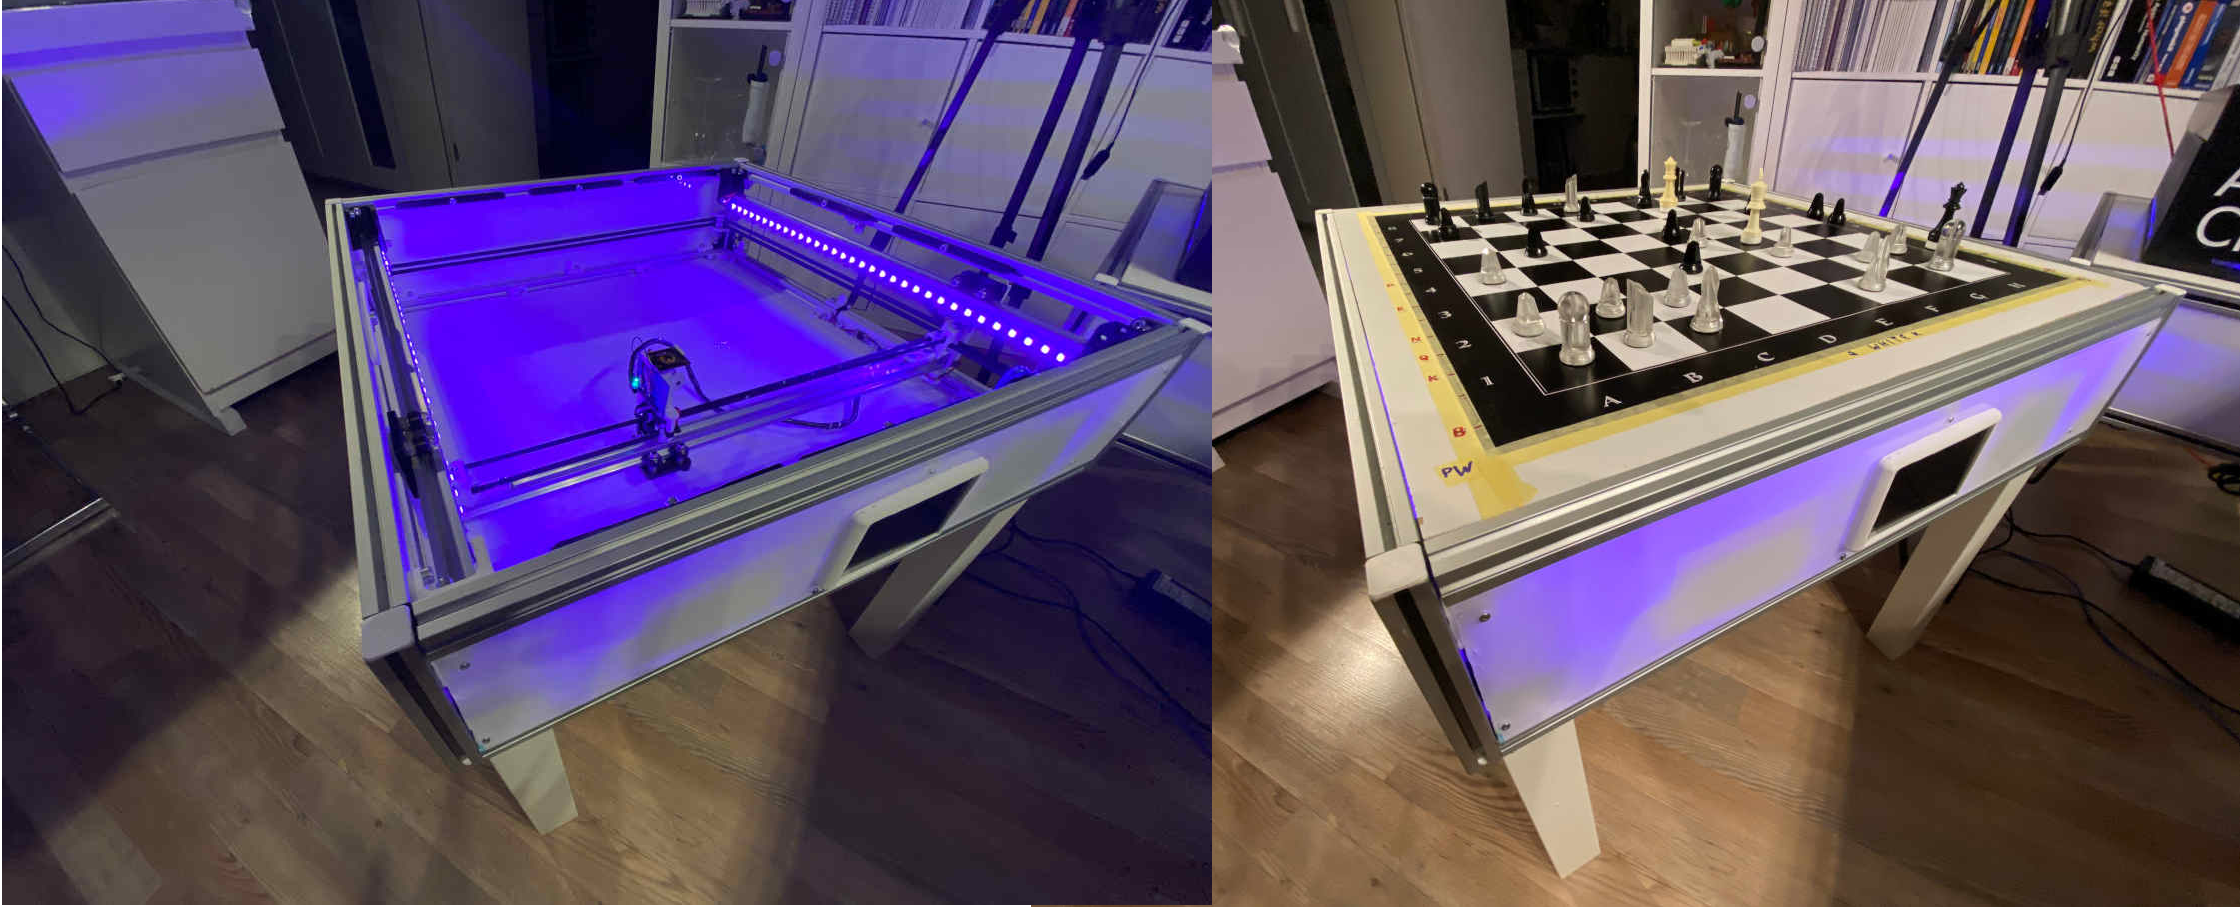
\includegraphics{images/table_images/prod.png}
\caption{Producation Hardware: Finaler autonomer Schachtisch
\label{prod}}
\end{figure}

\hypertarget{modifikation-der-mechanik}{%
\section{Modifikation der Mechanik}\label{modifikation-der-mechanik}}

\hypertarget{gehuxe4use-und-design}{%
\subsection{Gehäuse und Design}\label{gehuxe4use-und-design}}

Mit der Entscheidung, auf die hölzerne Struktur des Systems gänzlich zu
verzichten, wurden massive Veränderungen des Designs des Schachtischs
bestehend aus Gehäuse, Dimensionen und allen Außenelementen nötig.

Zuvor bestand der Quader-förmige Schachtisch aus einem Lack-Tisch als
Deckel, welcher mit einem selbsterstellten Untergestell bestehend aus
Rahmen und Boden verschraubt wurden. Nun muss der Quader selbst
konstruiert werden.

Die Wahl des neuen Materials war jedoch simpel; aufgrund der
langjährigen Bewährtheit, der Stabilität und der einfachen Möglichkeit
der Anpassung wurde als Basis des neuen System Aluminium-Profilstangen
gewählt. Da der Tisch keine größeren Kräfte aufnehmen muss, wurde ein
Stangengrundmaß von 20 x 20 mm gewählt. Diese sind dennoch stabil genug,
um möglichen Außeneinwirkungen wie Stößen oder Drücken standzuhalten.

Als Außenmaße wurden 620 x 620 x 170 mm (Länge, Breite, Höhe) gewählt.
Das Außenmaß ergab sich aus der Berechnung der benötigten
Spielfeldgröße, der Parkpositionen und der gegebenen Stangenbreite. Die
Schachfiguren besitzen einen maximalen Durchmesser von 22 mm. Damit
Figuren einander ohne Berührung vorbeigeführt werden können, ist somit
eine Größe von mindestens 44 mm für ein Feld nötig. Da eine Distanz
eingerechnet werde muss, um ein Anziehen der Figuren zu verhindern und
Fehler bei der mittigen Positionierung der Figuren möglich sind, wurde
hierfür eine zusätzliche Toleranz von 13 mm ergänzt und somit ein
Idealmaß von 57 mm Seitenlänge pro Feld errechnet. Bei einem
vollständigen Schachtisch ergibt sich daraus eine Schachfeldgröße von
456 x 456 mm. Für die Parkpositionen wurden zusätzlich noch einmal 30 mm
berechnet mit einem Abstand zum Feld von weiteren 37 mm. Somit ergibt
sich, wenn man das Feld quadratisch auslegt, eine Seitenlänge von 590
mm. Als Plattenmaß wurde 620mm gewählt, um eine Toleranz für die
Befestigung zu Berücksichtigen und zudem mögliche Einschränkungen der
Mechanik vorzubeugen.

Die Platte wird dann in Alu-Profilstangen eingelassen; die Stangen
sollen die Platte umrahmen. Mit einem Grundmaß von 20 x 20 mm für die
Profilstangen ergibt sich somit ein Gesamtmaß von 660 mm x 660 mm.
Benötigt werden 8 Profilstangen der Länge 620 mm und 4 der Länge 170 mm,
welche zu einem Quadratischen Kasten zusammengesetzt werden. Für die
X-Achsen werden zudem zwei Profilstangen der Länge 610 mm und für die
Y-Achse noch eine weitere der Länge 620 mm benötigt.

Die für die Montage üblicherweise verwendeten Winkel wurden jedoch
aufgrund der Größe nicht verwendet. Es wurden eigene Winkel mittels
3D-Druck erstellt oder auch Komponenten zur Befestigung direkt als
Winkel-Elemente integriert. So wird der obere Quadrant des Korpus von 4
Winkel gehalten, welche zum einen als Auflage für die Tischplatte
fungieren und zum anderen das Befestigen der beiden X-Achsen
Profilstangen dient.

Da die Tischpatte nur aufliegt, ist es zusätzlich möglich, den Raum
unterhalb der Profilstangen als Konstruktionsraum zu verwenden. Dabei
ist zu beachten, dass an allen Seiten des Tischens noch Seitenelemente
bestehend aus 620 x 130 x 5 mm Acrylglas-Platten eingelassen werden.
Somit beträgt die exakte Länge der für die Konstruktion nutzbaren Seiten
650 mm. Lediglich die Ecken, welche die Höhenelemente der Aluprofile
beinhalten, bieten nur eine Länge von 620 mm.

Um das Design optisch zu verbessern, wurden die Acrylglas-Elemente in
weiß gewählt. Transparente Elemente ermöglichen zwar eine Sicht auf die
Mechanik im Inneren, jedoch wurde hierbei insbesondere Wert auf den
Gesamteindruck gelegt, welcher durch die weiße Struktur des Glases
aufgewertet wird. Zudem wurden im Inneren noch zusätzlich LED-Streifen
verlegt, welche dank des verwendeten TMC-Boards einfach angeschlossen
werden konnten. Die weißen Glaselemente streuen das Licht günstiger und
ermöglichen so ein unterschwelliges Leuchten.

Um das System vollständig zu verschließen und somit auch besser zu
schützen wurde zudem eine Bodenplatte mit identischen Maßen zur
Tischplatte eingelassen und mit Stützelementen verschraubt.

Nachteil der verwendeten Aluminium-Profilstangen und der weißen
Acrylglas-Elemente sind die höheren Kosten und der Aufwand. Der
verwendete Lack-Tisch und auch das selbsterstellte Untergestell als
solche waren preisgünstig und leicht erhältlich, zudem war die
Tischplatte, welche aus einem einzelnen Tisch bestand, stabil und
robust. Aluminiumstangen hingegen, die zusätzlich noch bestellt,
selbstständig an die gewünschte Länge angepasst und mit weiteren
Komponenten verschraubt werden müssen, sind dementsprechend deutlich
kostenintensiver.

Zudem wurde die Tischplatte nun durch eine simple Holzplatte ersetzt.
Eine Höhe von 3 mm darf aufgrund des Magnetismus zwischen Schlitten und
Schachfigur nicht überschritten werden. Um ein Durchbiegen dieser zu
verhindern wurden in den Profilstangen horizontale Vorsprünge ergänzt,
die die Platte auf einer Ebene mit der Oberkante der Alu-Profilstangen
halten.

Die Beine des zuvor verwendeten Lack-Tischs wurden erneut verwendet;
diese konnten für die zweite Revision verwendet werden und so zusätzlich
die gleiche Montagehöhe zwischen der ersten und der zweiten Revision
erreicht werden. Da selbst die Höhe der Quader des Schachtischs
identisch ist, sind beide Tische nun gleich hoch. Eine Alternative
Lösung wäre der Erwerb von simplen Hohlleisten der gleichen Länge oder
aber das Integrieren weiterer Profilstangen, welche man optimaler Weise
auch klappbar lagern könnte. Derzeit sind die Beine verschraubt und
nicht klappbar. Der daraus resultierende Nachteil der Tischbeine ist,
dass man den gesamten Tisch nun schwerlich auf einen anderen Tisch
stellen kann, um die Montage zu erleichtern oder ein Schachspiel auf
einer anderen, eventuell bequemeren Höhe durchzuführen. Da hingegen
benötigt der Tisch nun keine Unterlage mehr und kann ohne Probleme im
offenen Raum platziert werden. Die aktuell verwendeten Beine können je
nach Bedarf auch entfernt werden, sodass der Schachtisch wieder als
simpler Quader einfach zu handhaben ist.

Dennoch überwiegen die Vorteile der Universalität dank der gegebenen
Normungen, der einfachen Anpassungsmöglichkeiten in der Länge und dem
einfachen Ergänzen und Verschieben von Komponenten. Im Holzrahmen
verschraubte Elemente hinterlassen Löcher, die zu Beeinträchtigungen
führen können. Zudem ist das Ergänzen von anderen Komponenten im
Aluminium-Profil einfacher.

\hypertarget{d-komponenten}{%
\subsection{3D-Komponenten}\label{d-komponenten}}

Die Masse an selbst-erstellten 3D-Komponenten wurde aufgrund des selbst
erstellten Korpus in der zweiten Revision erhöht. Aluprofile bieten die
Möglichkeit der einfachen Montage von zusätzlichen Komponenten. Mittels
sogenannter Nutensteine, welche in das Profil geschoben werden, ist es
möglich, diese Komponenten einfach an das Profil zu Schrauben, indem man
in das im Nutenstein befindliche Gewinde schraubt. Dank der
Schienen-ähnlichen Gestaltung der Profile sind die Positionen dieser
Nutensteine individuell anpassbar. Ausgehend von den gewählten Maßen der
Stangen wurden Nutensteine vom „Typ 6`` mit einem M5 Gewinde gewählt.

Zudem wurde nur ein einziges 3D-Design angefertigt, indem eine simple
Platte erstellt wurde, auf welcher zwei Vorsprünge extrudiert wurden und
eine Durchführung des Durchmessers 6,5 mm. Mittels der Durchführung
konnte die Platte mit einem Nutenstein verschraubt werden, mittels der
Vorsprünge, welche in die Profilschienen ragen, wird ein Drehen der
Platte verhindert. Dieses 3D-Design wurde für Folgenden als Grundlage
für alle neuen Komponenten genommen. Oftmals wurden bestehende Modelle
der ersten Revision mit diesem neuen Design verbunden und als eine
Komponente gedruckt, was eine Wiedernutzung von etablierten Komponenten
ermöglicht.

Der Grundrahmen als solcher wurde einmalig erstellt und nur in einfachen
Strukturen wie der Winkel-Sehnenlängen oder Höhenparametern von Flächen
angepasst. Alle weiteren Komponenten im Inneren bedurften mehrerer
Revisionen, um die verwendete Mechanik optimal umzusetzen und mehr
Kräfte für Riemenspannungen zu ermöglichen.

Insgesamt benötigt der gesamte Schachtisch 26 verschiedene mittels FDM
3D-gedruckte Komponenten, durch Mehrfachnutzung werden insgesamt 75
Elemente gedruckt. Dies ergab bei den verwendeten Druckern und dem
gewählten Filament eine Druckzeit von 25 Stunden und rund 450 Gramm
Filament.

Zusätzlich zu diesen Komponenten ist es möglich, 32 Schachfiguren
mittels SLA 3D-Druck zu erzeugen.

\hypertarget{positions-mechanik}{%
\subsection{Positions-Mechanik}\label{positions-mechanik}}

Die Mechanik des ersten Prototypens wurde für die Erstellung des zweiten
Prototypens gänzlich verändert. In der ersten Revision wurde noch jede
Achse über einen separaten Riemen gesteuert, sodass ein Schrittmotor die
Bewegung des Schlittens entlang der Y-Achse und ein weiterer die
Bewegung der gesamten Y-Achse, bestehend aus Motor, Riemen, Schlitten
und Führungsschiene, entlang der X-Achse ermöglicht. Die Führung entlang
der X-Achse erfolgt in der Mitte des Tischs, die Y-Achse wurde links und
rechtsseitig rollbar gelagert und in der Mitte über einen Riemen
gezogen. Dies hat zur Folge, dass bei entstehender Unwucht, welche durch
die Bewegung des Schlittens auf der Y-Achse natürlich ist, die Y-Achse
in ihren Lagerungen nicht mehr parallel verläuft, sondern beim Betätigen
des Motors der X-Achse die Y-Achse in einem unerwünschten Winkel bewegt
wird.

Die Konsequenz dessen ist, dass die Schachfiguren nicht mehr rein
parallel zu X oder Y-Achse bewegt werden konnten, sondern immer ein
unvorteilhafter Winkel in den Bewegungsablauf integriert wurde. Das
hatte zur Folge, dass Figuren nicht richtig positioniert wurden oder zu
dicht an unbewegten Figuren vorbeigeführt wurden.

Eine Lösungsmöglichkeit wäre die Ergänzung eines zweiten Motors für die
X-Achse, sodass linksseitig und rechtsseitig unmittelbar an der Lagerung
gezogen werden kann. Dies erwies sich jedoch als unpraktikabel und würde
einen zusätzlichen Kostenfaktor darstellen. Ein stabileres Befestigen
der Y-Achse in ihren Lagerungen hatte zur Folge, dass der Widerstand der
Lagerungen zunahm und die Bewegung der Achse nur unter erhöhten Kräften
möglich war.

Deswegen wurde ein völlig anderes System für die zweite Revision des
Schachtischs gewählt, welche auf beide Achsen die gleichen Kräfte ausübt
und beide Achsen nicht mehr unabhängig voneinander betrachtet.

CoreXY basiert auf der Idee alter Zeichentische und wird heute für
verschiedene Anwendungen wie den 3D-Druck oder das \gls{cnc}-Fr genutzt,
bei dem ein Objekt oder Werkzeug in mehreren Dimensionen bewegt werden
soll.

Ein Objekt wird von zwei Enden desselben gespannten Riemens gehalten;
wenn ein Ende des Riemens kürzer wird, wird das andere Ende länger. Der
Riemen wird über Lagerungen in den gegenüberliegenden Ecken eines
Rechtecks so angeordnet, dass die Bewegung eines Motors eine Bewegung
des Werkzeugs in einem 45-Grad-Winkel bewirkt. Werden nun zwei Riemen in
das System gebracht und alle vier Enden an dem Objekt befestigt, so ist
es möglich, durch das Bewegen des einen Riemens mittels einer Bewegung
des anderen Riemens den 45-Grad Winkel zu einer geraden Strecke zu
glätten. Das bedeutet, dass man beide Motoren bewegen muss, um in einer
geraden Linie zu fahren.

Einer der größten Vorteile des CoreXY-Systems ist die hohe
Bewegungsgeschwindigkeit. Dies ist insbesondere dadurch möglich, es
keine beweglichen Teile von nennenswerter Masse gibt. In der ersten
Revision wurde beim Bewegen der X-Achse alle Komponenten bewegt, zu
denen auch der höher gewichtige Schrittmotor zählt. Im neuen System ist
die einzige Belastung der Schlitten und dessen Lagerung, die beiden
Motoren sind in gegenüberliegenden Ecken des Tisches dauerhaft befestigt
und dienen jeweils als ein Lagerpunkt (und Antriebspunkt) eines Riemens.
Nur die Lagerung der Y-Achse hat leichte Reib-Einflüsse. Das bedeutet,
dass der Schlitte der einzige Teil des Systems ist, der mit einer
nennenswerten Geschwindigkeit und Masse bewegt wird, und dass daher viel
weniger Vibrationen auftreten.

Da die Riemen des Systems dauerhaft auf Spannung gehalten werden, ist
kein Spiel mehr im System festzustellen. Positionen der Schachfiguren
werden Millimetergenau und mit einer hohen Wiederholgenauigkeit
angefahren.

Ein weiterer Vorteil ist, dass CoreXY das gleiche Bauvolumen bei
geringeren Gesamtabmessungen bieten kann. Der Fahrweg der Schachfiguren
konnte somit ausgeweitet werden, ohne den Bauraum des Tisches zu ändern,
da bei einem CoreXY-System jeder Punkt der gesamten Bauplatte angefahren
werden kann, ohne zusätzlichen Platz zu benötigen. Bei einem Außenmaß
des Tisches von 620x620 mm wies der erste Prototyp einen Fahrweg von
480x480 mm auf, während die zweite Revision mit selben Außenmaßen einen
Fahrweg von 580x580 mm erreicht. Der Fehlende Raum der ersten Version
ist insbesondere auf die Lagerung der Motoren zurückzuführen, die
jeweils ihre eigene Achse verkürzten. Nun liegen beide Motoren auf der
x-Achse und dienen sogar als Bremse vor den Steuerkomponenten.

Die Konstruktion ist zudem stabiler, es erleichtert das Einschließen und
Aufstellen im ausgeschalteten Zustand.

Zudem ist die Steuerung des CoreXY-Systems bereits in der Firmware
Marlin integriert. Es ist lediglich in den Parametern CoreXY zu
aktivieren und die Schrittweiten auszurechnen. Wird anschließend eine zu
fahrende Strecke vorgegeben, berechnet Marlin selbständig, wie schnell
und in welche Richtung jeder der beiden Motoren bewegt werden muss.

In der Komplexität des Aufbaus und dessen Zeitaufwand war kein
Unterschied zwischen der ersten und zweiten Revision zu erkennen. Für
Anfänger im Bereich CoreXY ist das Verlegen und insbesondere das stramme
Spannen der Riemen eine Herausforderung, die sich aber durch die
Konstruktion der Bauteile vereinfachen lässt. Insbesondere die
Verbindung an der Lagerung der Y-Achse ist so erstellt worden, dass die
Riemen nach der Durchführung nur in eine definierte Richtung gespannt
werden können.

Das Resultat übertrifft sogar die Erwartungen. Die Mechanik ist robust
und es konnten keine Fehler mehr im Betrieb festgestellt werden.
Einzelne Fehler durch nachgiebige 3D-Konstruktionen wurden ausgebessert
und so ein optimales und möglichst beständiges X-Y-System erzeugt.

\hypertarget{optimierungen-der-spielfiguren}{%
\section{Optimierungen der
Spielfiguren}\label{optimierungen-der-spielfiguren}}

\begin{figure}
\centering
\includegraphics{images/ATC_ChessFigures.png}
\caption{Schachfiguren im Vergleich \label{ATC_ChessFigures}}
\end{figure}

Die bisher genutzten vorgefertigten Figuren funktionierten grundsätzlich
gut mit dem ersten Prototyp. Allerdings wiesen sie eine zu hohe
Fehleranfälligkeit, in Bezug auf das gegenseitige Beeinflussen
(abstoßen, anziehen) durch die verwendeten Magnete auf. Zusätzlich
stellt der Fertigungsprozess einer Figur einen zeitlichen Aufwand dar,
diese jeweils aus fünf \ref{ATC_ChessFigures} Einzelteilen bestehen:

\begin{itemize}
\tightlist
\item
  Figur
\item
  Basisplatte
\item
  Magnet
\item
  \gls{nfc} Tag
\item
  Filzgleiter
\end{itemize}

Die Größe der Figuren kann durch die fest definierte Schachfeldgröße von
57mm und der verwendeten \gls{nfc} Tags nicht verändert werden. Nach
einigen Testdurchläufen mit dem ersten Prototyp war zu erkennen, dass
sich die Figuren je nach aktueller Situation auf dem Spielfeld weiterhin
magnetisch anziehen. Um diesen Fehler zu beheben wurden verschiedenen
Bewegungsgeschwindigkeiten getestet, ergaben allerdings für diesen
Anwendungsfall keine merkliche Verbesserung.

Dies führt je nach Spielverlauf zu Komplikationen, sodass die Figuren
manuell vom Benutzer wieder mittig auf den Felder platziert werden
müssen. Um dies zu verhindern, wurde einige Figuren zusätzlich mit einer
20mm Unterlegscheibe am Boden beschwert. Diese behob das Problem, jedoch
erwies sich das \gls{nfc} Tag nicht mehr als lesbar.

Die aktuell verwendeten Figuren des ersten Prototyps wiegen zwischen 8
Gramm für die Bauern und 10 Gramm für die restlichen Figuren. Der Test
mit der Unterlegscheibe ergab das diese mit 5 Gramm zusätzlich genug
Gewicht hinzufügen, um die magnetische Beeinflussung zu unterbinden.

Testweise wurden einige Figuren mittels 3D Drucker erstellt, um so das
Gewicht zu erhöhen. Nach einem erfolgreichen Test wurde das \gls{cad}
Modell so angepasst, dass sich der Magnet direkt in den Boden der Figur
einkleben lässt. Des Weiteren wurden bei den Bauern die Magnete
ausgetauscht. Die zuerst verwendeten 10x3mm Neodym-Magnete wurden bei
diesen Figuren gegen 6x3mm Magnete getauscht. Somit sind im Design zwei
verschiedenen Arten von Magneten notwendig, jedoch traten in den
anschließend durchgeführten Testläufen keine Beeinflussungen mehr auf.

Durch diese Veränderungen am Figur-Design, konnte zusätzlich die Zeit
für den Zusammenbau einer einzelnen Figur gesenkt werden. Es werden nur
noch vier \ref{ATC_ChessFigures} Einzelteile (Figur, Magnet, NFC-Tag,
Filzgleiter) verwendet und zusätzliches verkleben dieser ist nicht mehr
notwendig. Diese können direkt in den Fuß der Figur mittels einer
Presspassung eingelegt werden.

\hypertarget{uxe4nderungen-der-elektronik}{%
\section{Änderungen der Elektronik}\label{uxe4nderungen-der-elektronik}}

Mit ein relevanter Kritikpunkt, welcher bereits während des Aufbaus des
ersten Prototyps zu erkennen war, ist die Umsetzung der Elektronik.
Diese wurde im ersten Prototyp manuell aufgebaut und enthielt viele
verschiedene Komponenten.

Die verwendeten Motortreiber stellten sich während der Entwicklung als
sehr flexibel heraus, stellten aber auch einen signifikanten
Kostenfaktor dar. Nach dem Aufbau und Erprobung des ersten Prototyps
wurde ersichtlich, dass hier nicht alle zuerst angedachten Features der
Treiber benötigt werden und so auch Alternativen in Betracht gezogen
werden konnten. Zusätzlich konnte die Elektronik nur beschränkt mit
anderen Systemen verbunden werden, was insbesondere durch die verwendete
\gls{spi} Schnittstelle geschuldet war.

All diese Faktoren erschweren einen einfachen Zusammenbau des autonomen
Schachtischs. Die Lösung stellt die Verwendung von Standardhardware dar.
Nach der Minimierung der elektrischen Komponenten und des mechanischen
Aufbaus ist zu erkennen, dass der autonome Schachtisch einer
\gls{cnc}-Fr bzw. eines 3D Drucker stark ähnelt. Insbesondere die
XY-Achsen Mechanik sowie die Ansteuerung von Schrittmotoren wird in
diesen Systemen verwendet. Mit dem Durchbruch von 3D Druckern im
Konsumer-Bereich sind auch kleine und preisgünstige Steuerungen
\ref{3dmarlinctl} erhältlich, welche 2-3 Schrittmotoren und diverse
zusätzliche Hardware ansteuern können.

Hierbei existiert eine große Auswahl dieser mit den verschiedensten
Ausstattungen. Bei der Auswahl dieser wurde vor allem auf die
Möglichkeit geachtet sogenannte Silent-Schrittmotortreiber verwenden zu
können, um die Geräuschimmissionen durch die Motoren so weit wie möglich
zu minimieren. Im ersten Prototyp wurde unter anderem aus diesem Grund
die \passthrough{\lstinline!TMC5160-BOB!} Treiber ausgewählt. Die
meisten Boards bieten austauschbare Treiber, so ist es auch im
nachhinein möglich diese auszuwechseln.

\begin{longtable}[]{@{}lccr@{}}
\caption{Standardhardware 3D Drucker Steuerungen
\label{3dmarlinctl}}\tabularnewline
\toprule
& SKR 1.4 Turbo & Ramps 1.4 & Anet A8 Mainboard\tabularnewline
\midrule
\endfirsthead
\toprule
& SKR 1.4 Turbo & Ramps 1.4 & Anet A8 Mainboard\tabularnewline
\midrule
\endhead
Stepper Driver & TMC2209 & A4988 / TMC2209 & A4988\tabularnewline
LED Strip Port & WS2811 / RGB & - & -\tabularnewline
Firmware & Marlin-FW 2.0 & Marlin-FW 1.0 & Proprietary\tabularnewline
\bottomrule
\end{longtable}

Hierzu wurde der Schrittmotor-Treiber \passthrough{\lstinline!TMC2209!}
gewählt, welcher diese Features ebenfalls unterstützt und in der
Variante als Silent-Step-Stick direkt in die meisten 3D Drucker
Steuerungen eingesetzt werden können. Hierbei ist es wichtig, dass auf
der gewählten Steuerung die Treiber-ICs nicht fest verlötet sind,
sondern getauscht werden können. Ein weiterer Punkt ist die
Kommunikation der Steuerung mit dem Host-System. Hierbei setzten alle
untersuchten Steuerungen auf die \gls{usb} Schnittstelle und somit ist
eine einfache Kommunikation gewährleistet. Das verwendete eingebettete
System im autonomen Schachtisch bietet vier freie \gls{usb} Anschlüsse,
somit ist eine einfache Integration gewährleistet.

\begin{figure}
\centering
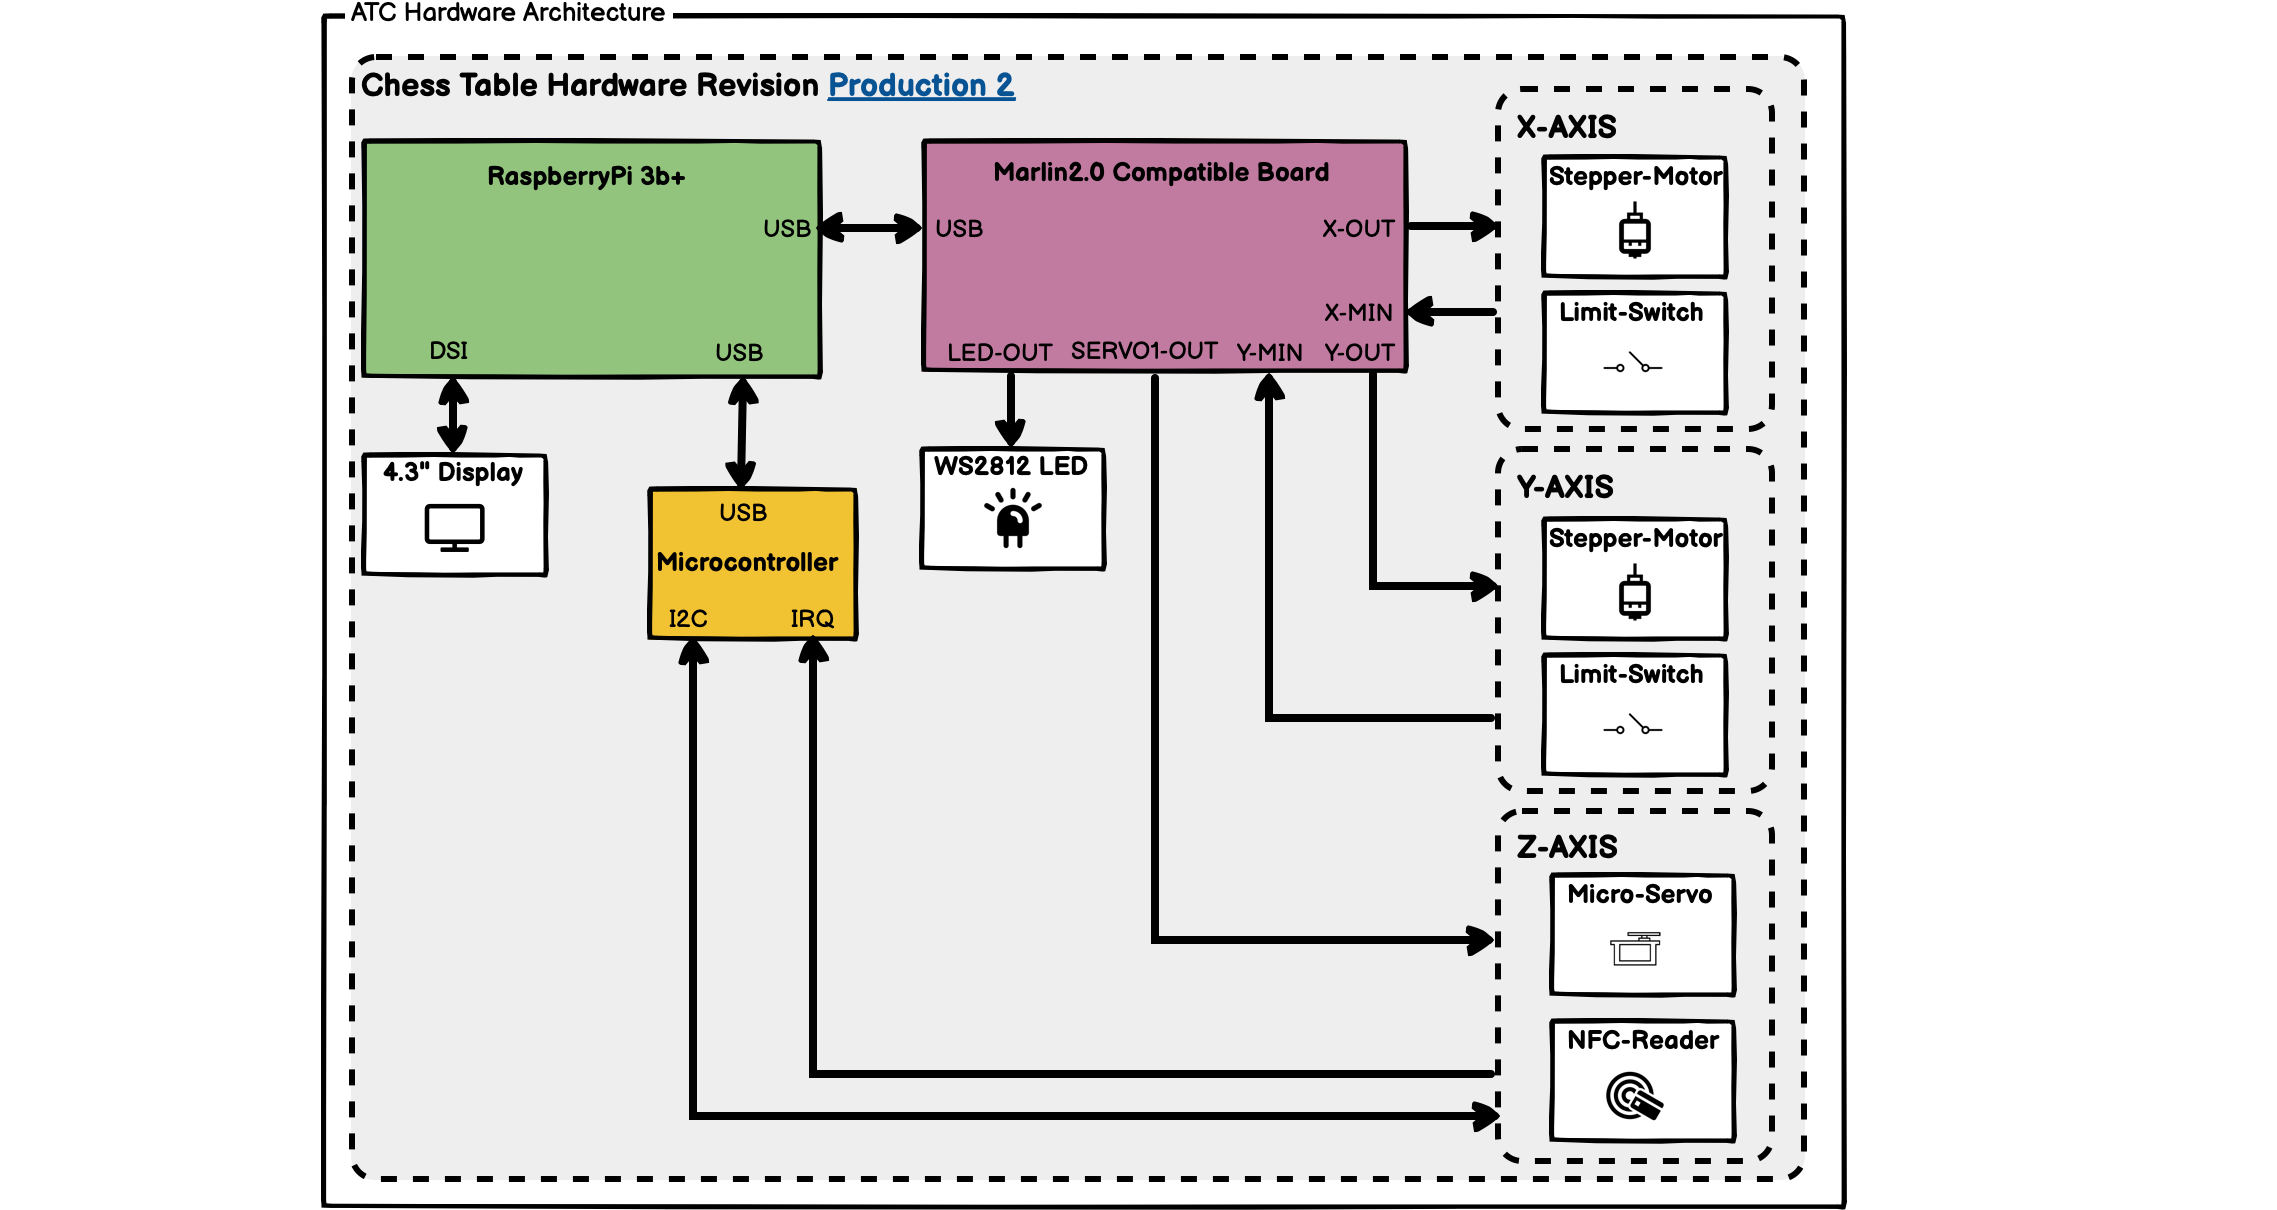
\includegraphics{images/ATC_Hardware_Architecture_PROD.png}
\caption{Producation Hardware: Blockdiagramm
\label{ATC_Hardware_Architecture_PROD}}
\end{figure}

Nach einer gründlichen Evaluation der zur Verfügung stehenden
Steuerungen, wurde die \passthrough{\lstinline!SKR 1.4 Turbo!}-Steuerung
ausgewählt, da diese trotz des geringfügig höheren Marktpreises genug
Ressourcen auch für spätere Erweiterung bietet und eine Unterstützung
für die neuste Version der Marlin-FW\cite{marlinfw} bereitstellt.
Somit wurde die Elektronik durch die verwendete Plug\&Play stark
vereinfacht \ref{ATC_Hardware_Architecture_PROD}.

\hypertarget{anpassungen-hal}{%
\section{Anpassungen HAL}\label{anpassungen-hal}}

\hypertarget{implementierung-gcode-sender}{%
\subsection{Implementierung
GCODE-Sender}\label{implementierung-gcode-sender}}

Durch die durchgeführten Änderungen an der Elektronik insbesondere durch
die Verwendung einer Marlin-FW\cite{marlinfw} fähigen
Motorsteuerung, ist eine Anpassung der \gls{hal} notwendig. Diese
unterstütz die Ansteuerung der Motoren und anderen Komponenten (z.B.
Spindeln, Heizelemente) mittels G-Code und wird typischerweise in 3D
Druckern und \gls{cnc}-Fr eingesetzt.

G-Code ist eine Programmiersprache, welche mittels einfacher Befehle
textbasierten Befehle \ref{gcodecmd}, Komponenten dieser Maschienen
kontrollieren kann. Dabei können einzelne Achsen verfahren werden oder
die Drehzahl einer Spindel kontrolliert werden. Der G-Code wird von der
Steuerung interpretiert. In der Regel wird dieser zuvor von einem
\gls{cad} Programm erzeugt und Zeilenweise übertragen. Bei einem 3D
Drucker wird dieser vom Slicer generiert und enhält die Wegpunkte welche
von dem Hotend angefahren werden sollen.

Im falle des autonomen Schachtisch, werden die G-Code Anweisungen
on-the-fly durch die \gls{hal} erzeugt und die Motorsteuerung verfährt
die Achsen an die jeweils gewünschten Positionen.

Marlin-FW\cite{marlinfw} biete dabei einen großen Befehlssatz an
G-Code Kommandos an. Bei diesem Projekt werden jedoch nur einige G-Code
Kommandos verwendet \ref{gcodecmd}, welche sich insbesondere auf die
Ansteuerung der Motoren beschränken.

\begin{longtable}[]{@{}lcr@{}}
\caption{Grundlegende verwendete G-Code Kommandos
\label{gcodecmd}}\tabularnewline
\toprule
& G-Code Command & Parameters\tabularnewline
\midrule
\endfirsthead
\toprule
& G-Code Command & Parameters\tabularnewline
\midrule
\endhead
Move X Y & G0 & X\passthrough{\lstinline!dest\_pos\_x\_mm!}
Y\passthrough{\lstinline!dest\_pos\_y\_mm!}\tabularnewline
Move Home Position & G28 & -\tabularnewline
Set Units to Millimeters & G21 & -\tabularnewline
Set Servo Position & M280 & P\passthrough{\lstinline!servo\_index!}
S\passthrough{\lstinline!servo\_position!}\tabularnewline
Disable Motors & M84 & X Y\tabularnewline
\bottomrule
\end{longtable}

Die erforderlichen Kommandos wurden auf ein Minimum beschränk, um eine
maximale Kompatibilität bei verschiedenen G-Code-fähigen Steuerungen zu
gewährleisten. Die Software unterstützt jedoch weitere Kommandos wie
z.B. \passthrough{\lstinline!M150!} mit welchem speziellen Ausgänge für
\gls{led}s gesteuert werden können. Dieses Feature bietet sowohl die
verwendete Marlin-FW\cite{marlinfw} als auch die verwendete
Steuerung an. Sollte die verwendete Steuerung solch ein optionales
Kommando nicht unterstützen, so werden diese ignoriert was zur Folge
hat, dass auch preisgünstige Steuerungen verwendet werden können.

Die Kommunikation zwischen Steuerung und eingebetteten System geschieht
durch eine \gls{usb} Verbinden. Die Steuerung meldet sich als virtuelle
Serielle Schnittstelle im System an und kann über diese mit der Software
kommunizieren. Auch werden so keine speziellen Treiber benötigt, da auf
nahezu jedem System ein Treiber \passthrough{\lstinline!USB-CDC!} für
die gängigsten \gls{usb} zu seriell Wandler bereits installiert ist. Die
Software erkennt anhand der zur Verfügung stehenden \gls{usb}-Ger sowie
deren Vendor und Product-\gls{id} Informationen die verbundene Steuerung
und verwendet diese nach dem Start automatisch. Hierzu wurde zuvor eine
Liste \ref{gcodeusbctl} mit verschiedenen getesteten Steuerungen sowie
deren \gls{usb}-Vendor und Product-\gls{id} angelegt.

\begin{longtable}[]{@{}lccr@{}}
\caption{Hinterlegte G-Code Steuerungen
\label{gcodeusbctl}}\tabularnewline
\toprule
Product & Vendor-ID & Product-ID & Board-Type\tabularnewline
\midrule
\endfirsthead
\toprule
Product & Vendor-ID & Product-ID & Board-Type\tabularnewline
\midrule
\endhead
Bigtreetech SKR 1.4 Turbo & 1d50 & 6029 &
Stepper-Controller\tabularnewline
Bigtreetech SKR 1.4 & 1d50 & 6029 & Stepper-Controller\tabularnewline
Bigtreetech SKR 1.3 & 1d50 & 6029 & Stepper-Controller\tabularnewline
\bottomrule
\end{longtable}

Damit die Software mit der Steuerung kommunizieren kann, wurde eine
G-Code Sender Klasse implementiert, welche die gleichen Funktionen wie
die \gls{hal}-Basisklasse bereitstellen. Nach Aufruf einer Funktion zum
Ansteuern der Motoren, wird aus den übergebenen Parametern das passende
G-Code Kommando in Form einer Zeichenkette zusammengesetzt und auf die
Serielle Schnittstelle geschrieben.

\begin{lstlisting}[language={C++}]
//GCodeSender.cpp
bool GCodeSender::setServo(const int _index,const int _pos) {
    return write_gcode("M280 P" + std::to_string(_index) + " S" + std::to_string(_pos));
}

bool GCodeSender::write_gcode(const std::string _gcode_line, bool _ack_check) {
    //...
    //FLUSH INPUT BUFFER
    port->flushReceiver();
    //APPEND NEW LINE CHARAKTER IF NEEDED
    if (_gcode_line.rfind('\n') == std::string::npos)
    {
        _gcode_line += '\n';
    }
    //WRITE COMMAND TO SERIAL LINE
    port->writeString(_gcode_line.c_str());
    //WAIT FOR ACK
    return wait_for_ack();
}

bool GCodeSender::wait_for_ack() {
    int wait_counter = 0;
    //...
    while (true) {
        //READ SERIAL REPONSE
        const std::string resp = read_string_from_serial();
        //...
        //PROCESS RESPONSE
        if (resp.rfind("ok") != std::string::npos)
        {
            break;
        }else if(resp.rfind("echo:Unknown") != std::string::npos) {
            break;
        }else if(resp.rfind("Error:") != std::string::npos) {
            break;            
        }else if (resp.rfind("echo:busy: processing") != std::string::npos) {
            wait_counter = 0;
            LOG_F("wait_for_ack: busy_processing");
        }else {
            //READ ERROR COUNTER AND HANDLING
            wait_counter++;
            if (wait_counter > GCODE_ERROR_RETRY_COUNT)
            {
                break;
            }
        }
    }
    //...
    return true;
}
\end{lstlisting}

Die Steuerung verarbeitet diese und bestätigt die Ausführung mit einer
Acknowledgement-Antwort. Hierbei gibt es verschiedenen Typen. Der
einfachste Fall ist ein \passthrough{\lstinline!ok!}, welches eine
erfolgreiche Abarbeitung des Kommandos signalisiert. Ein weiterer Fall
ist die Busy-Antwort \passthrough{\lstinline!echo:busy!}. Diese
Signalisiert, dass das Kommando noch in der Bearbeitung ist und wird im
Falle des autonomen Schachtisches bei langen und langsamen Bewegungen
der Mechanik ausgegeben. Das System wartet diese Antworten ab bis eine
finale \passthrough{\lstinline!ok!}-Antwort zurückgegeben wird, erst
dann wird das nächste Kommando aus der Warteschlange bearbeitet.

\hypertarget{i2c-seriell-umsetzer}{%
\subsection{I2C-Seriell Umsetzer}\label{i2c-seriell-umsetzer}}

Durch den Wegfall der zuvor eingesetzten Elektronik und der Austausch
durch die \passthrough{\lstinline!SKR 1.4 Turbo!} Steuerung, ist jedoch
ein Anschluss des \passthrough{\lstinline!PN532!} \gls{nfc} Moduls nicht
mehr direkt möglich, da dieses mittels \gls{i2c} Interface direkt mit
dem eingebetteten System verbunden war. Dieses Interface entfällt nun.
Dennoch besteht weiterhin die Möglichkeit, jedoch wurde auch hier auf
eine \gls{usb} Schnittstelle gewechselt. So ist es möglich das System
auch an einem anderen Host-System zu betreiben, wie z.B. an einem
handelsüblichen Computer.

Dazu wurde ein Schnittstellenwandler entwickelt welcher die \gls{i2c}
Schnittstelle zu einer \gls{usb} Seriell wandelt. Indes wurde ein
\passthrough{\lstinline!Atmega328p!} Mikrokontroller eingesetzt, da
dieser weit verbreitet und preisgünstig zu beschaffen ist. Die Firmware
des Mikrokontroller stellt ein einfaches kommandobasiertes Interface
bereit. Die Kommunikation ist mit der Kommunikation und der
Implementierung des G-Code Senders vergleichbar und teilen sich die
gleichen Funktionen zur Kommunikation mit der Seriellen Schnittstelle.

\begin{lstlisting}[language={C++}]
//userboardcontroller.cpp Atmega328p Firmware
//simplyfied version
char scan_nfc_tag(){
    //...
    if (nfc.tagPresent())
    {
        //READ TAG CONTENT
        NfcTag tag = nfc.read();
        //READ NDEF PAYLOAD
        NdefMessage msg = tag.getNdefMessage();
        if(msg.getRecordCount() > 0){
            //READ FIRST RECORD
            NdefRecord record = msg.getRecord(0);
            const int payloadLength = record.getPayloadLength();
            byte payload[payloadLength];
            //...
            record.getPayload(payload);
            //...
            //...
            //RETURN FIGURE ID
            if(payloadLength == 6){
                return payload[3];
            }
        }
    return 0; //VALID TAGS FROM 1-127
}
\end{lstlisting}

In diesem Falle wird nur ein Befehl zum Auslesen des \gls{nfc} Tags
benötigt. Das Host-System sendet die Zeichenkette
\passthrough{\lstinline!\_readnfc\_!} zum Mikrokontroller und dieser
versucht über das \passthrough{\lstinline!PN532!} Modul ein \gls{nfc}
Tag zu lesen. Wenn dieses erkannt wird und einen passenden Payload
enthält, antwortet dieser mit dem String
\passthrough{\lstinline!\_readnfc\_res\_FIGURE-ID\_ok\_!} oder wenn kein
Tag gefunden wurde mit
\passthrough{\lstinline!\_readnfc\_red\_\_empty\_!}. Auch hier wird wie
bei der G-Code Sender Implementierung auf Fehler bei der Kommunikation
bzw. einem Abbruch durch einen Timeout reagiert. Das System
initialisiert die Serielle Schnittstelle neu und resettet das System
durch setzten des \passthrough{\lstinline!DTR!}-\gls{gpio} am
\gls{usb}-Seriell Wandler \gls{ic} (falls vorhanden).

\begin{lstlisting}[language={C++}]
//UserBoardController.cpp HOST-SYSTEM
ChessPiece::FIGURE UserBoardController::read_chess_piece_nfc(){
    ChessPiece::FIGURE fig;
    fig.type = ChessPiece::TYPE::TYPE_INVALID;
    //...
    //READ SERIAL RESULT
    const std::string readres = send_command_blocking(UBC_COMMAND_READNFC);
    //...
    //SPLIT STRING _
    const std::vector<std::string> re = split(readres,UBC_CMD_SEPERATOR);
    //READ SECTIONS
    //...
    const std::string figure = re.at(3);
    const std::string errorcode = re.at(4);
    //CHECK READ RESULT
    if(errorcode == "ok"){
        if(figure.empty()){
            break;
        }
        //...
        //DETERM FINAL READ FIGURE
        const char figure_charakter = figure.at(0);
        fig = ChessPiece::getFigureByCharakter(figure_charakter);
    }
    //...
    return fig;
}
\end{lstlisting}

Das System erkennt den Anschluss der Hardware beim Start auf die gleiche
Art und Weise wie der G-Code Sender. Dafür wurden einige verschiedene
Mikrokontroller im System hinterlegt \ref{umbdctl}, auf welchen die
Firmware getestet wurde.

\begin{longtable}[]{@{}lccr@{}}
\caption{Hinterlegte Mikrokontroller \label{umbdctl}}\tabularnewline
\toprule
Product & Vendor-ID & Product-ID & Board-Type\tabularnewline
\midrule
\endfirsthead
\toprule
Product & Vendor-ID & Product-ID & Board-Type\tabularnewline
\midrule
\endhead
Arduino Due {[}Programming Port{]} & 2341 & 003d &
User-Move-Detector\tabularnewline
Arduino Due {[}Native SAMX3 Port{]} & 2341 & 003e &
User-Move-Detector\tabularnewline
CH340 & 1a86 & 7523 & User-Move-Detector\tabularnewline
HL-340 & 1a86 & 7523 & User-Move-Detector\tabularnewline
STM32F411 & 0483 & 5740 & User-Move-Detector\tabularnewline
\bottomrule
\end{longtable}

\hypertarget{fazit-bezuxfcglich-des-finalen-prototypens}{%
\section{Fazit bezüglich des finalen
Prototypens}\label{fazit-bezuxfcglich-des-finalen-prototypens}}

Der in der zweiten Iteration entstandene Prototyp wurde in viele
Elemente aus der ersten Iteration grundlegend überarbeitet. Dabei
endstand ein völlig neues Design, welches sich auf einfach zu
beschaffende Komponenten und Materialien stützt. Diese ermöglichen einen
simpleren und zeitlich effektiven Zusammenbau des vollständigen
autonomen Schachtischs und bieten die Möglichkeit auf eine einfache
Erweiterung des Systems.

Aus der Verwendung des CoreXY Aufbaus resultierte eine nahezu spiel- und
verlustfreie Mechanik (+-1mm), welche für diesen Zweck überaus geeignet
ist. Somit konnten die mechanischen Probleme vom ersten Prototyp
vollständig eliminiert werden und führen somit zu einer zuverlässigen
Spielführung. Diese Zuverlässigkeit wurde im mehreren Testläufen
verifiziert und ein abschliessender sechs Stunden Dauertest bestätigt
diese zusätzlich. Auch konnte die Bewegungsgeschwindikeit des Schlittens
erhöht werden, was zu einem schnelleren Platzieren der Figuren führt.

Ein großer Kritikpunkt des ersten Prototypens war die nicht vollständig
funktionsfähigen Park-Positionen für die ausgeschiedenen Figuren. Durch
die Vergrößerung des Bewegungsspielraums der Achsen und der Anpassungen
in der Software, ist es nun möglich, alle Figuren vom Spielbrett
entfernen zu können. Das System ist darauffolgend auch in der Lage,
diese wieder in das Spielgeschehen zurückholen zu können. Somit ist kein
manuelles Eingreifen durch den Benutzer mehr notwendig, wenn ein neues
Spiel gestartet werden soll.

Zusätzlich wurde durch das transparente Design eine neue Art der
Benutzerinteraktion geschaffen. Durch die visuellen Hinweise, welcher
der Tisch mittels der \gls{led} Beleuchtung geben kann, ist der Nutzer
nicht mehr auf die \gls{gui} angewiesen und erfährt visell, ob der
gegnerische Spielzug beendet wurde. Der Nutzer kann ohne Aufwand
erkennen, in welchem Zustand sich der autonome Schachtisch befindet.

Zudem konnte eine reibunglose Erkennung des getätigten Schachzug
umgesetzt werden, welches bei der vorherigen Version nicht vollständig
umsetzbar war. Durch den modularen Aufbau der \gls{hal} und des
erweiteren Revisions-Management ist es zudem möglich, die Software auf
allen bisher erstellen Prototypen ausführen zu können.

Somit ist festzuhalten, dass mit der zweiten Revision alle zuvor
geforderten Eigenschaften \ref{finalfeaturesatc} zufriedenstellend
umgesetzt werden konnten. Die erstellte Hard- und Software bietet
zusätzliche zahlreiche Erweiterungsmöglichkeiten.

\begin{longtable}[]{@{}lr@{}}
\caption{Eigenschaften die finalen Prototypen
\label{finalfeaturesatc}}\tabularnewline
\toprule
& \gls{atc} -- autonomous Chessboard\tabularnewline
\midrule
\endfirsthead
\toprule
& \gls{atc} -- autonomous Chessboard\tabularnewline
\midrule
\endhead
Feldabmessungen (LxBxH) & 57x57mm\tabularnewline
Abmessungen (LxBxH) & 620x620x170mm\tabularnewline
Gewicht & 5.7kg\tabularnewline
Konnektivität & \gls{wlan}, \gls{usb}\tabularnewline
Automatisches Bewegen der Figuren & ja\tabularnewline
Erkennung Schachfigurstellung & ja\tabularnewline
Spiel Livestream & ja\tabularnewline
Cloudanbindung (online Spiele) & ja\tabularnewline
Parkposition für ausgeschiedene Figuren & ja\tabularnewline
Stand-Alone Funktionalität & ja\tabularnewline
Besonderheiten & visuelle Hinweise per Beleuchtung\tabularnewline
\bottomrule
\end{longtable}

Dennoch ist zu beachten, dass dieser Stand des Projekts noch nicht
vollständig ausgereift ist und noch Verbesserungspotential bietet,
welche zum Beispiel vor einem kommerziellen Verkauf des Produktes
notwendig wären. Dabei besonders markant ist die Erkennung der vom
Benutzer getätigten Schachzüge. Durch die Verwendung des \gls{nfc}
Moduls und dem Scanvorgang des Schachfeldes muss eine gewisse Wartezeit
von ca. 20 Sekunden in Kauf genommen werden, bevor das System einen Zug
erkennt. Somit sind keine schnellen Partien möglich wie zum Beispiel
andere Schachformen wie das Schnellschach, bei denen die Zugzeit
begrenzt ist.

\hypertarget{entwicklung-der-cloud-infrastruktur}{%
\chapter{Entwicklung der Cloud
Infrastruktur}\label{entwicklung-der-cloud-infrastruktur}}

Die erste Phase der Entwicklung des Systems bestand in der Auslegung und
Erstellung der Cloud-Infrastruktur und der darauf ausgeführten Services.
Die ``Cloud'' stellt in diesem Zusammenhang einen Server dar, welcher
aus dem Internet über eine feste IPv4 und IPv6-Adresse verfügt und frei
konfiguriert werden kann. Auf diesem System ist der Schach-Cloud Stack
\ref{ATC_Cloud_Architecture} installiert, welcher zum einen aus der
Schach-Software besteht, welche in einem Docker-Stack ausgeführt wird
und zum anderen\ldots{}.

\begin{figure}
\centering
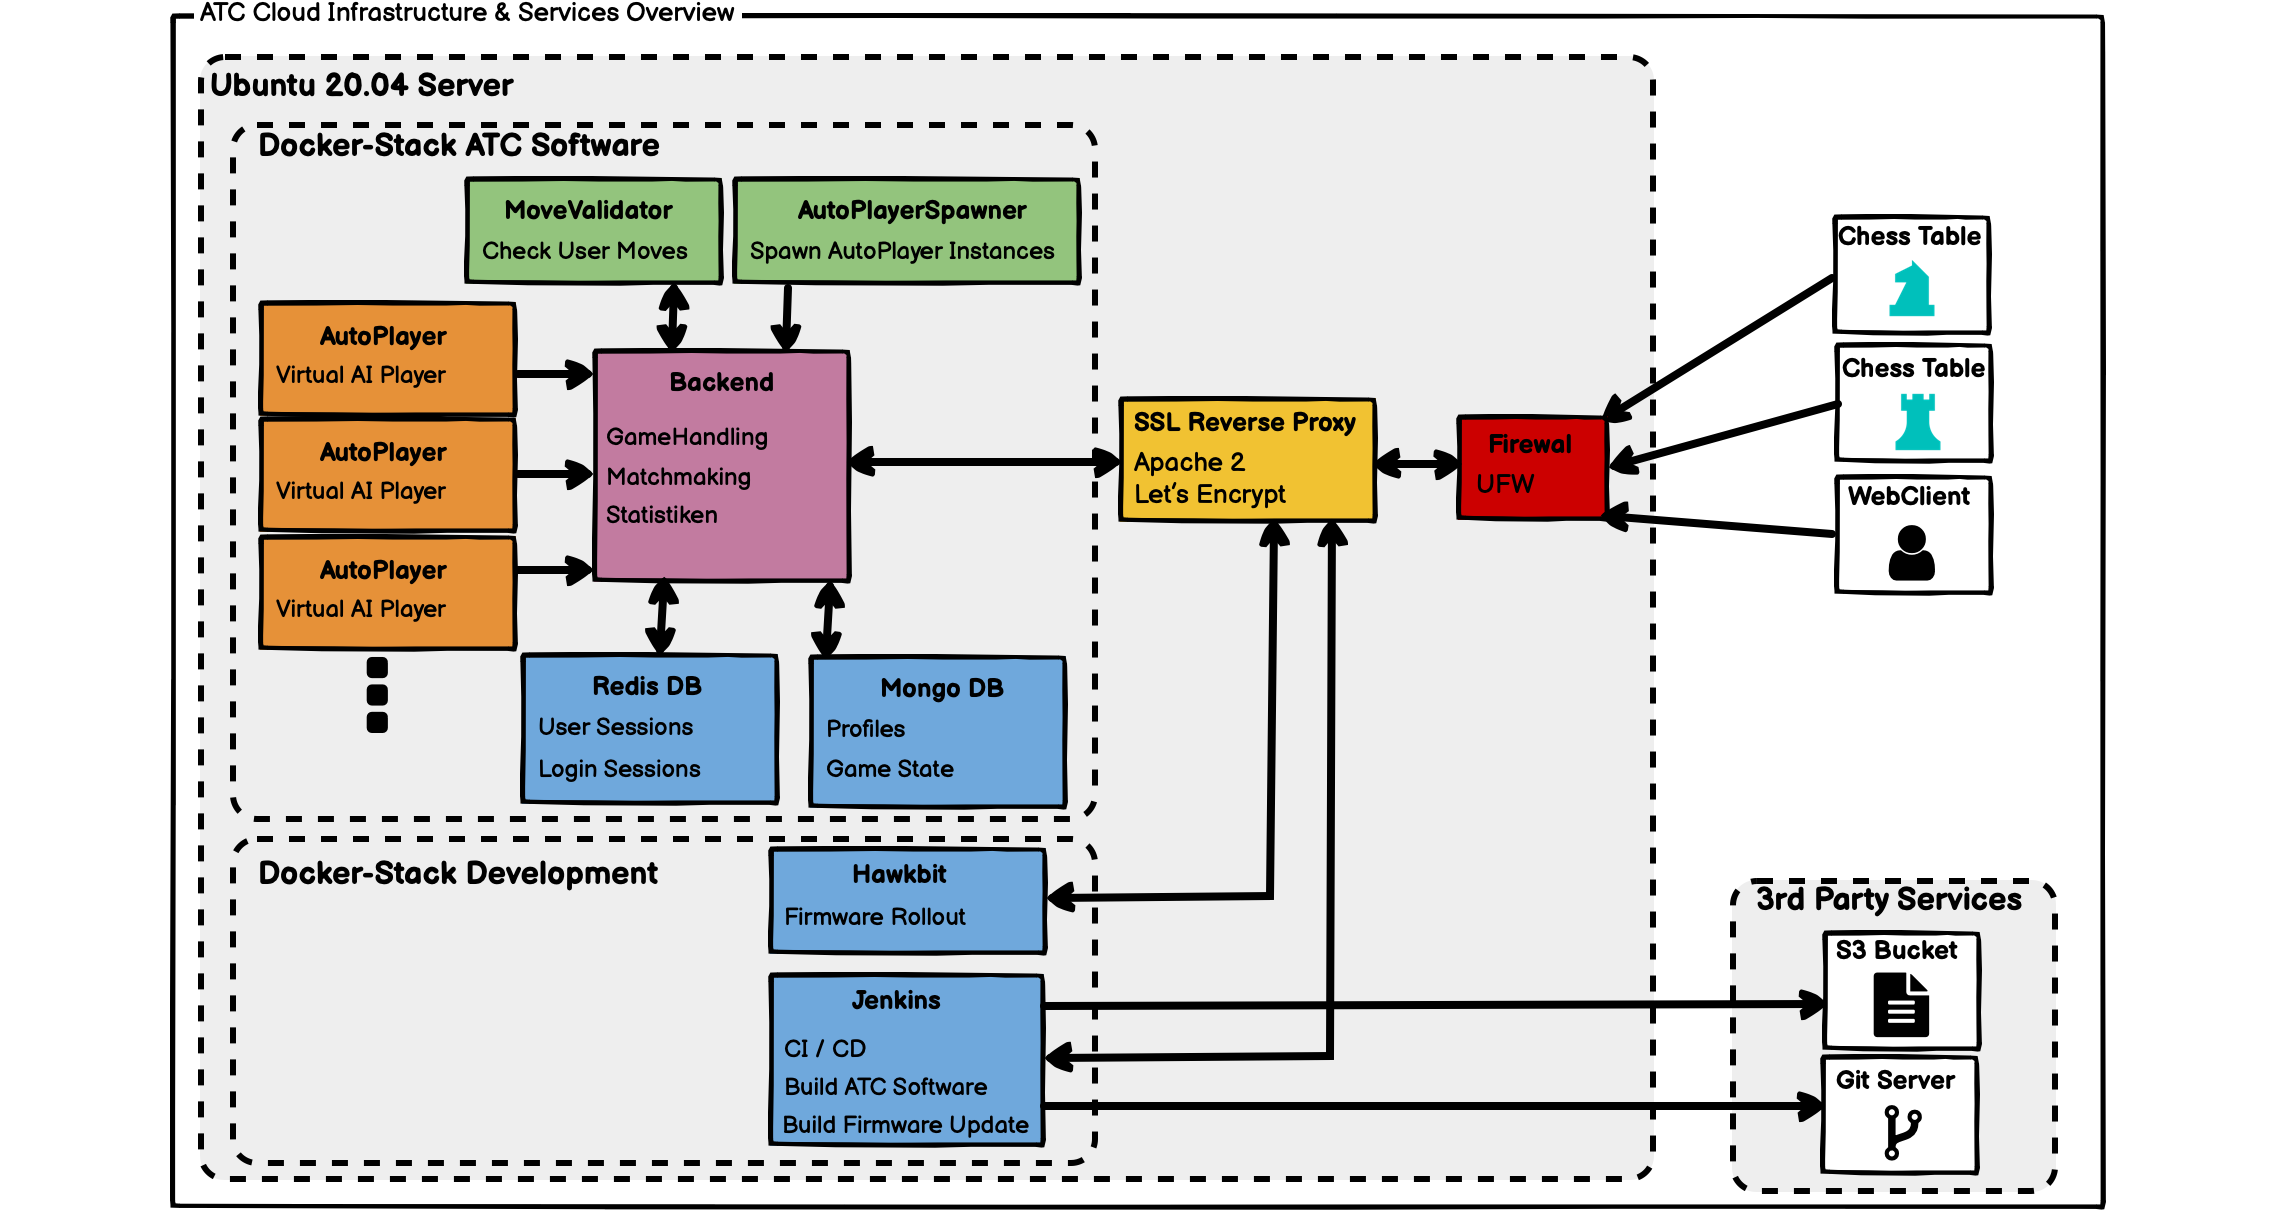
\includegraphics{images/ATC_Cloud_Architecture.png}
\caption{Gesamtübersicht der verwendeten Cloud-Infrastruktur
\label{ATC_Cloud_Architecture}}
\end{figure}

\hypertarget{api-design}{%
\section{API Design}\label{api-design}}

Das System soll so ausgelegt werden, dass es zu einem späteren Zeitpunkt
mit verschiedenen Client-Devices mit diesem kommunizieren können. Dazu
zählen zum einen der autonome Schachtisch, aber z.B. auch einen
Web-Client, welcher die Funktionalität eines Schachtisches im Browser
abbilden kann. Hierzu muss das System eine einheitliche
\gls{rest}-Schnittstelle bereitstellen.

\begin{figure}
\centering
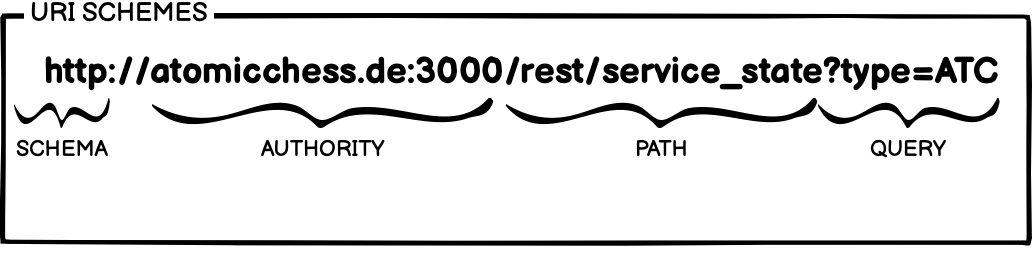
\includegraphics{images/ATC_URI_SCHEMES.png}
\caption{Cloud-Infrastruktur: Aufbau einer URI \label{ATC_URI_SCHEMES}}
\end{figure}

Die RESTful \gls{api} stellt verschiedene Ressourcen bereit, welche
durch eine URI \ref{ATC_URI_SCHEMES} eindeutig identifizierbar sind. Auf
diese können mittels verschiedenster HTTP Anfragemethoden (GET, POST,
PUT, DELETE) zugegriffen werden. Jeder dieser Methoden stellt einen
anderen Zugriff auf die Ressource dar und beeinflusst somit das
Verhalten und die Rück-Antwort dieser.

Eine URI besteht dabei aus mehreren Teilen. Das Schema gibt an wie die
nachfolgenden Teile interpretiert werden sollen. Dabei wird bei einer
RESTful Schnittstelle typischerweise das \gls{http} Protokoll, sowie
\gls{https} verwendet. Dabei steht \gls{https} für eine verschlüsselte
Verbindung.

Somit stellt die RESTful \gls{api} eine Interoperabilität zwischen
verschiedenen Anwendungen und Systemen bereit, welche durch ein Netzwerk
miteinander verbunden sind. Dieser Ansatz ist somit geeignet um die
verschiedenen Client Systeme (Schachtisch, Webclient) eine Kommunikation
mit dem Server zu erlauben.

\hypertarget{service-architektur}{%
\section{Service Architektur}\label{service-architektur}}

Der komplette Software-Stack, welcher zum Betrieb der Schach-Cloud
notwendig ist, wurde in einer sehr vereinfachten
Mikroservice-Archtivektur angelegt. Dies bedeutet, dass hier zum Betrieb
notwendige Softwarekomponenten in mehrere kleinere Bestandteile
ausgelagert wurden \ref{ATC_Service_Architecture}. Durch dieses modulae
Design ist es zusätzlich möglich, die eigentliche Schach-Logik auslagern
und in der Theorie auch andere Spiele implementieren zu können.

\begin{figure}
\centering
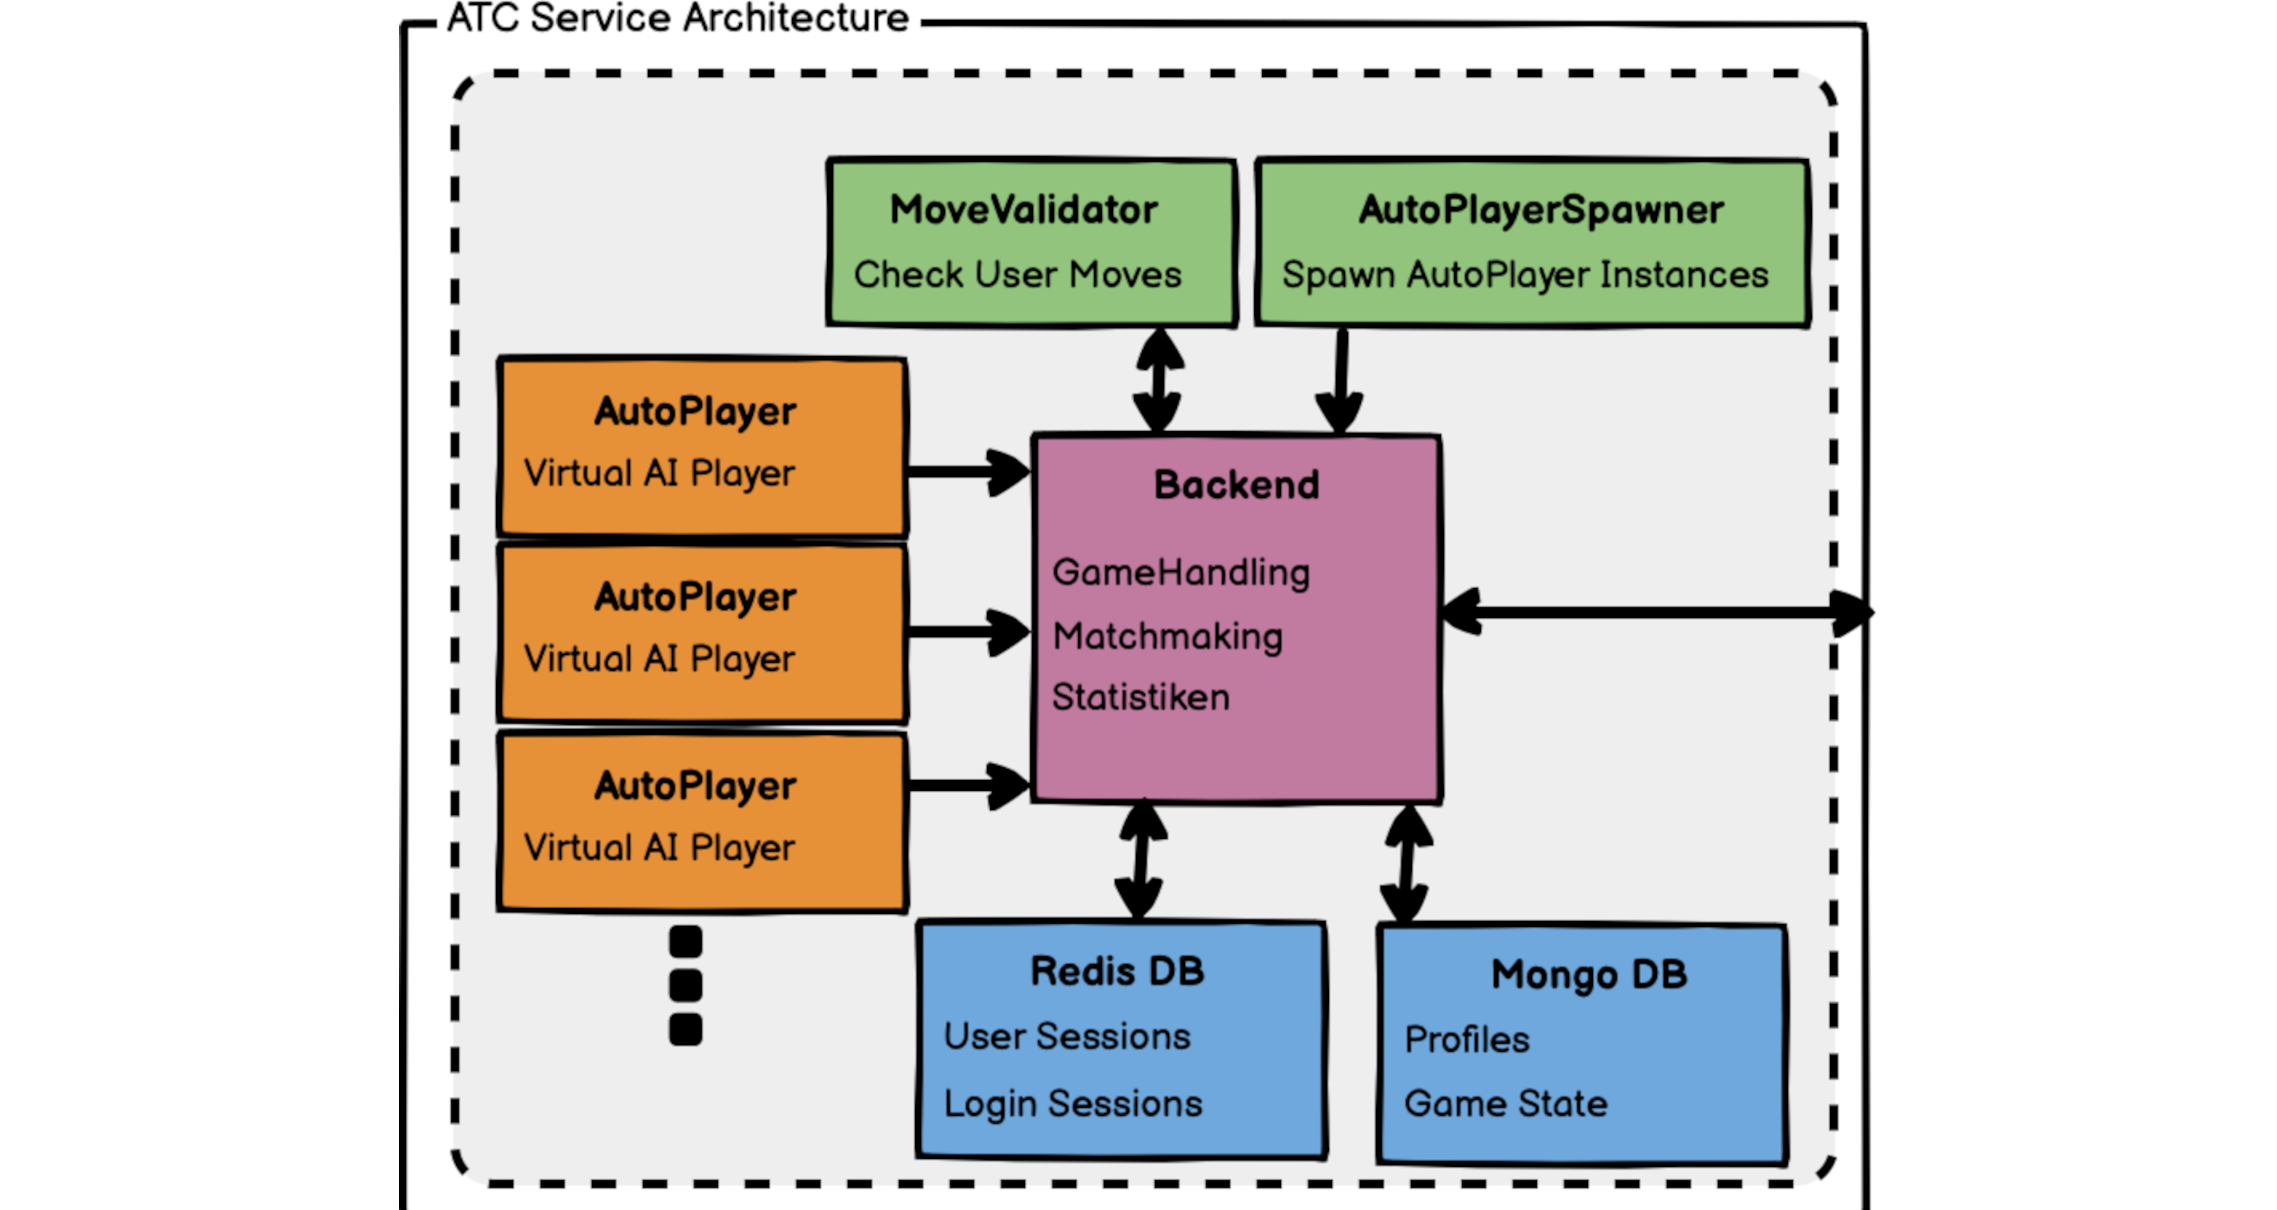
\includegraphics{images/ATC_Service_Architecture.png}
\caption{Cloud-Infrastruktur: Aufbau der Service Architecture
\label{ATC_Service_Architecture}}
\end{figure}

Diese einzelnen Komponent en sind eigenständig ausführbar und erst die
Vernetzung dieser in einem gemeinsamen privaten Netzwerk bilden eine
funktionfähige Schachcloud. Somit setzt sich diese aus den folgenden
Komponenten zusammen:

\begin{itemize}
\tightlist
\item
  Backend
\item
  MoveValidator
\item
  AutoPlayer
\end{itemize}

Da jede dieser Services stateless und und keine eigenen Daten speichert,
werden zwei Datenbank-Services benötigt um die Spieldaten zu speichern:

\begin{itemize}
\tightlist
\item
  Mongo NoSQL Datenbank
\item
  Redis In-Memory Key Value Datenbank
\end{itemize}

Hierbei wurde auf zwei verschiedenen Datenbanken gesetzt, welche im
Folgenden erläutert werden. Die \passthrough{\lstinline!Redis!}
\cite{redis} Datenbank wird ausschließlich für die Speicherung der
aktiven Sessions der einzelnen verbundenen Clients verwendet. Durch das
verwendete Sessionsystem, bei dem jeder Clients in kurzen Intervallen
seine aktivität bestätigen muss, bietet diese Datenbank den Vorteil,
dass diese durch ihre Archtiektur sehr schnell auf die angeforderten
Datensätze zugreifen kann. Auch wird hier nur der Datensatz gespeichert,
welche die notwendigen Informationen zu der aktiven Session des Clients
gespeichert. Diese werden durch die \gls{id} des Clients abgefragt.
Hierzu wird der Zeitstempel der Anmeldung, sowie die letzte Anfrage des
Clients in Form eines \gls{json} Dokuments gespeichert.

\begin{lstlisting}
{
 "client_hwid":"h34724",
 "login_ts": 1622128754,
 "heartbeat_ts":1622158754
}
\end{lstlisting}

Durch den Key-Value-Ansatz sowie den hohen Verbrauch an Arbeitsspeicher
eignet sich diese Datenbank jedoch nicht zum Speichern der Spieldaten.
Hierzu wurde ein zusätzlicher \passthrough{\lstinline!Mongo!}
\cite{mogodb} Datenbank Service erstellt, in welchem diese Daten
abgelegt werden. Zusätzlich zu den Spieldaten (Spiele, Spielstände,
Statistiken), werden auch die Nutzerprofile speichert. Ein Profile wird
beim ersten Anmeldevorgang erstellt und enthält neben den
Profilinformationen (Geräte-(id), Namen, Spielertyp) auch die Referenzen
auf die gewonnen und verlorenen Spiele. Die können später für die
Visualisierung verwendet werden.

Alle aufgelisteten Services werden in seperaten Containern betrieben.
Die Containervirtualisierung geschieht mittels der Software
\passthrough{\lstinline!Docker!} \cite{docker}. Diese stellt ein
einfaches Interface zur Erstellung von Containern und der Verwaltung
dieser. Um einen Container auf dem System starten zu können, muss dieser
zunächst aus einem Image heraus erstellt werden. Diese Image wird
mittels einer \passthrough{\lstinline!Dockerfile!} beschrieben und
besteht aus einer Reihe an Kommandos, welche den Aufbau des Images
beschreiben.

Bei diesem Projekt besteht ein Image in der Regel aus einem
vorgefertigten \passthrough{\lstinline!Ubuntu 20.04!} Image, in welchem
zusätzliche Software zur welche zur Ausführung der eingentlichen
Software benötigt wird. Auch existieren bereits vorgefertigte Images,
welche bereits Software für einen spezifischen Anwendungsfall enthält.

\begin{lstlisting}
# Dockerfile for ATC_AutoPlayer

FROM golang:latest #USE golang AS BASE IMAGE
RUN mkdir /app
ADD . /app/ # COPY SOURCE FILE OVER
WORKDIR /app
RUN ls
RUN cd ./stockfish-11-linux/src/ && make clean && make build ARCH=autodetect
RUN go mod init AutoPlayer ; exit 0
RUN CGO_ENABLED=0 GOOS=linux go build -a -installsuffix cgo -o main .
CMD ["/app/main"] # START APP
\end{lstlisting}

Da die Architektur aus mehr als einem Container besteht, gestaltet sich
eine manuelles Management dieser als nicht praktikabel. Zu diesem Zweck
existieren mehrere Tools und Systeme um solche Aufgaben zu
automatisieren. Ein weitere nicht zu vernachlässingender Punkt ist die
Abhänigkeit, welche unter den Container besteht. In diesem Fall benötigt
der Backend-Service die beiden Datenbanken um starten zu können. Somit
ist es essentiell, dass diese bereits zuvor erstellt wurden und
ausgeführt werden. Solche Funktionalitäten deckt das sehr
leichtgewichtigte Tool \passthrough{\lstinline!docker-compose!}
\cite{dockercompose} ab. Durch eine entsprechende
Konfiugrationsdatei, kann ein so genannter Stack aus mehreren Containern
aufgebaut werden.

\begin{lstlisting}
# docker-compose.yml STACK CONFIGURATION src_server
version: "3"
services:
  AtomicChessBackend:
    container_name: atcbackend
    depends_on:
      - AtomicChessRedisDatabase
      - AtomicChessMongoDatabase
      - AtomicChessMoveValidator
    links: 
      - "redisdb:AtomicChessRedisDatabase"
      - "mongodb:AtomicChessMongoDatabase"
      - "movevalidator:AtomicChessMoveValidator"
    image: atcbackend:latest
    build: 
      context: ../ATC_Backend/
    restart: always
    ports:
      - 3000:3000
    environment:
      - PRODUCTION=1

  AtomicChessMoveValidator:
    container_name: atcmovevalidator
    build:
      context: ../ATC_MoveValidator/
    image: atcmovevalidator:latest
    restart: always
    ports:
      - 5000:5000
    environment:
      - PRODUCTION

  AtomicChessRedisDatabase:
    image: redis:latest
    restart: always
    container_name: atcredis
    ports:
      - 6379:6379
    
  AtomicChessMongoDatabase:
    image: mongo:latest
    container_name: atcmongo
    restart: always
    environment:
        - MONGO_DATA_DIR=/data/db
        - MONGO_LOG_DIR=/dev/null
    volumes:
        - ./data/db:/data/db
    ports:
      - 27017:27017
    command: mongod --logpath=/dev/null # --quiet


  AtomicChessAutoPlayer:
    depends_on:
      - AtomicChessBackend
    links: 
        - "backend:AtomicChessBackend"
    build:
      context: ../ATC_AutoPlayer/
    image: atcautoplayer:latest
    restart: always
    scale: 5 # SPAWN THREE INSTANCES
    environment:
      - PRODUCTION=1
      - BACKEND_IP=backend:3000 #HOST IP:PORT OF BACKEND EXAMPLE 127.0.0.1:3000 USING ONLY HTTP
      #- USE_HOSTNAME_HWID=TRUE # USE THE LOCAL MACHINE HOSTNAME AS HWID
      #- PLAYER_TYPE_HUMAN=1 # SIMULATE A HUMAN PLAYER TYPE FOR TESTING
\end{lstlisting}

\hypertarget{service-backend}{%
\section{Service: Backend}\label{service-backend}}

\begin{figure}
\centering
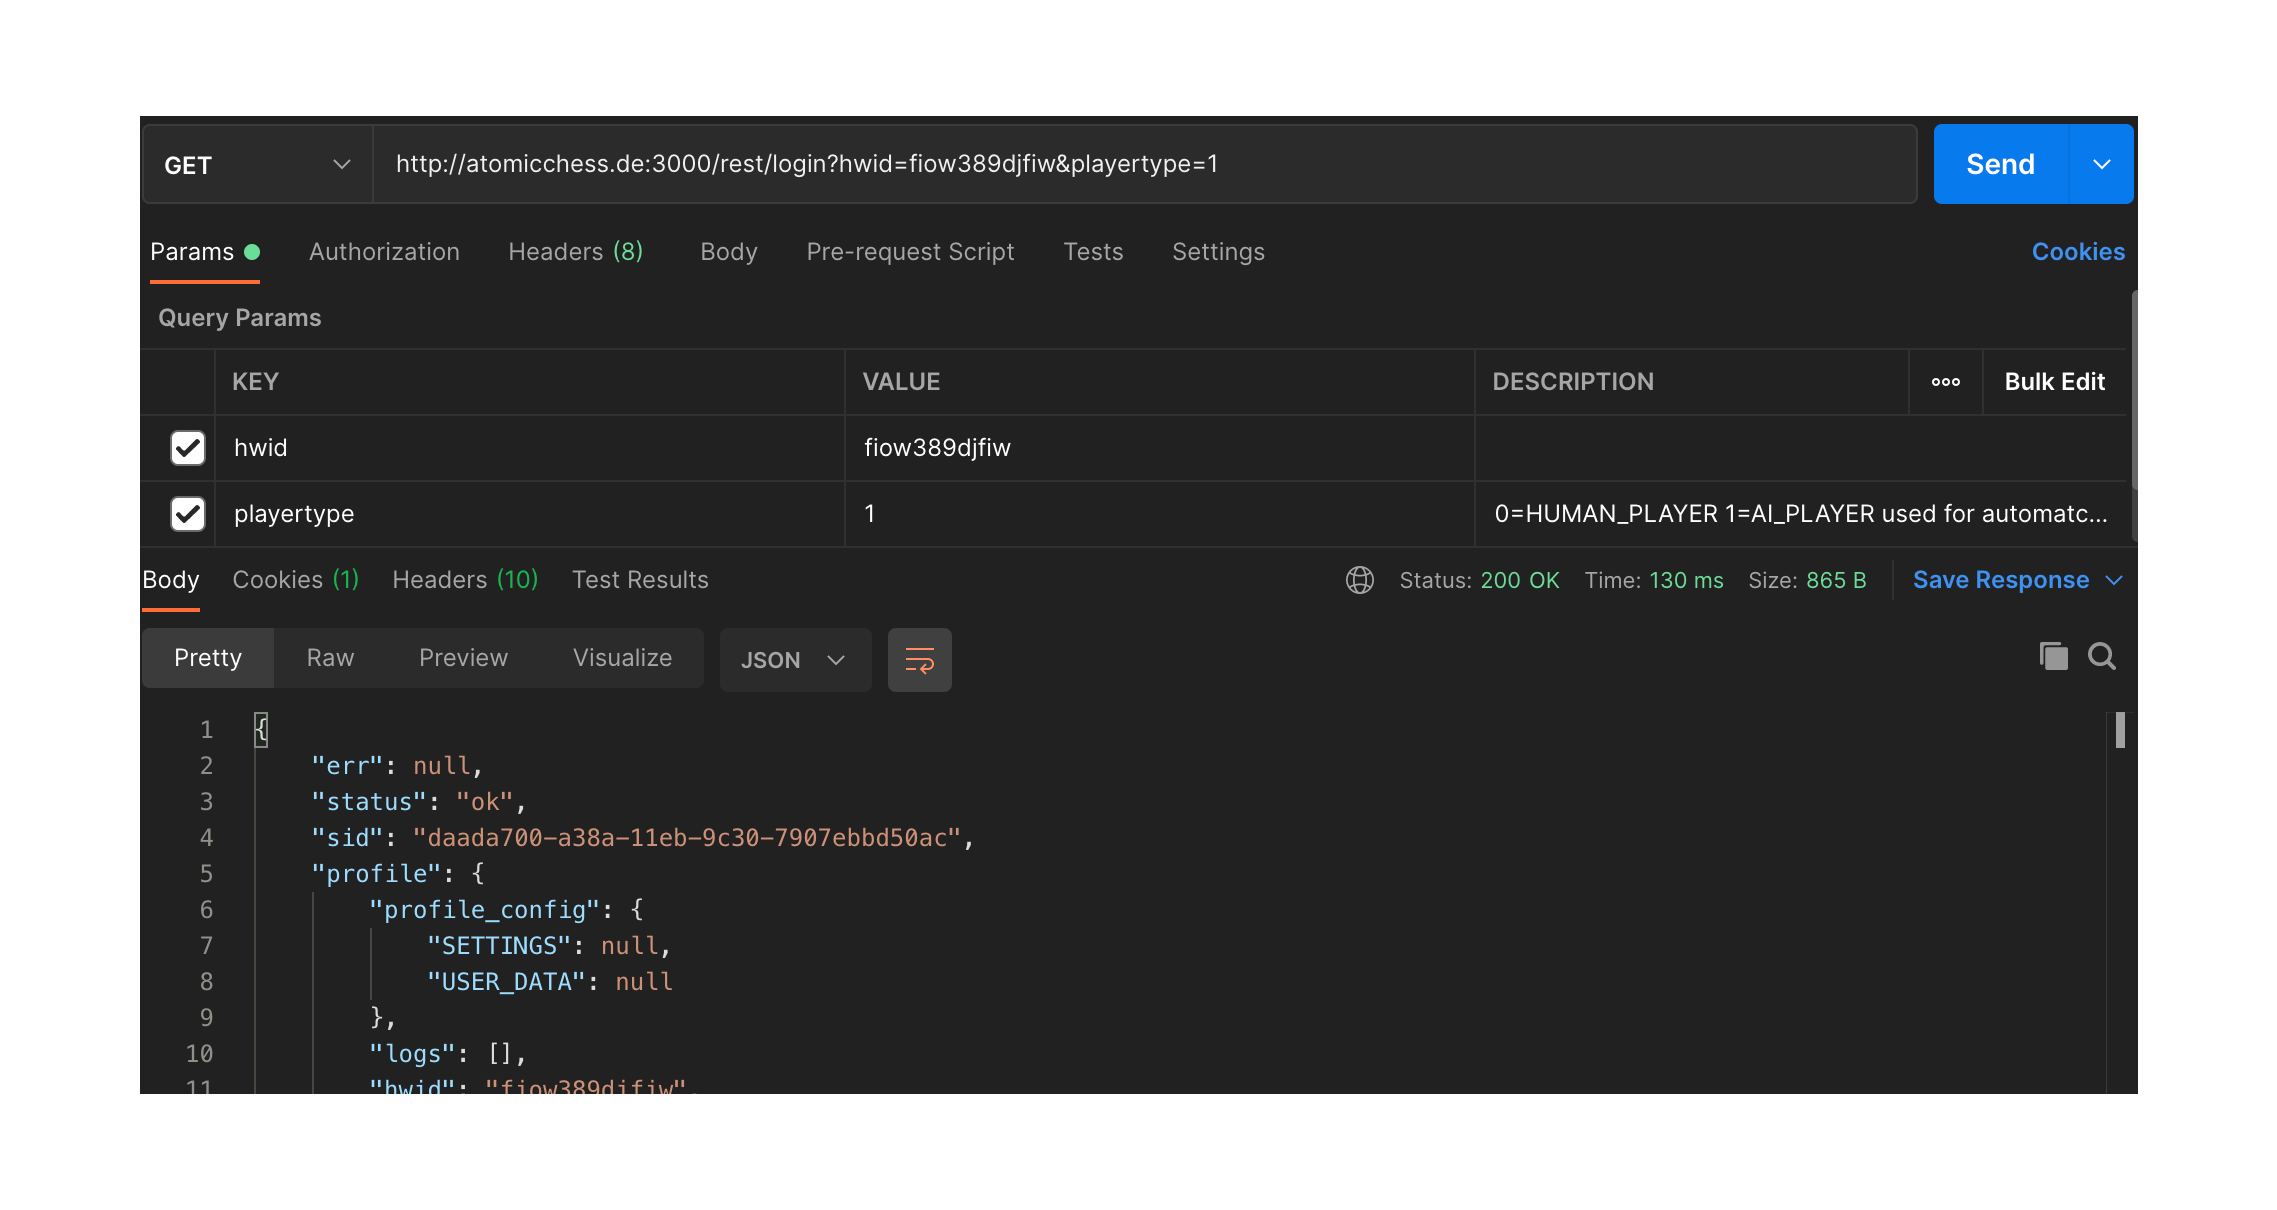
\includegraphics{images/ATC_request_example.png}
\caption{Cloud-Infrastruktur: Backend Login-Request und Response
\label{ATC_request_example}}
\end{figure}

Das Backend, welches den zentralen Teil der Service-Archtitektur bildet,
stellt den Zugriffspunkt für die autonomen Schachtische und den
Webclient (s.u.) dar. Diese stellt die \gls{api} zur Aussenwelt bereit,
mit dem sich die einzelnen Clients verbinden.

Dies geschieht zusätzlich durch einen \gls{tls}-Reverse Proxy, welcher
eine verschlüsselte Verbindung \gls{https} bereitstellt. Diese verwendet
zum einen eine self-signed Certificate, sowohl als auch ein Zertifikat
der Lets Entrypt Organisation\cite{letsencrpyt}. Somit ist die vom
Backend bereitgestellte \gls{api} und zum späteren Zeitpunt erstellen
Webclient (s.u.) für alle modernen Webbrowser vertrauenswürdig.

Bei dem eingerichteten Reverse-Proxy werden alle Verbindungen aus dem
öffentlichen Internet mit einem Service verbunden, welcher im lokalen
Netzwerk betrieben wird. In diesem Fall ist dies der lokale Server bzw
Localhost auf dem der Backend-Service auf dem Port 3000 ausgeührt wird.

\begin{lstlisting}
# APACHE 2 REVERSE PROXY CONFIGURATION
<IfModule mod_ssl.c>
<VirtualHost *:443>
        ServerName atomicchess.de
        ProxyPreserveHost On 
        DocumentRoot /var/www/html
        ProxyPass /.well-known !
        ProxyPass / http://127.0.0.1:3000/
        ProxyPassReverse / http://127.0.0.1:3000/    
    ServerAdmin webmaster@atomicchess.de

    ErrorLog ${APACHE_LOG_DIR}/error.log
    CustomLog ${APACHE_LOG_DIR}/access.log combined

    SSLCertificateFile /etc/letsencrypt/live/atomicchess.de/fullchain.pem
    SSLCertificateKeyFile /etc/letsencrypt/live/atomicchess.de/privkey.pem
    Include /etc/letsencrypt/options-ssl-apache.conf
</VirtualHost>
</IfModule>
\end{lstlisting}

Durch diese Methode wird eine sichere Verbindung zwischen dem Service
und dem Nutzer-Device hergestellt. Der Vorteil ist, dass die Services im
privaten Netzwerk keine \gls{tls} Zertifikate benötigen um in diesem
Netz miteinander kommunizieren zu können. Lediglich bei einer Verbindung
zum öffentlichen Internet wird eine sichere Verbindung durch die
Forward-Proxy Funktion des Apache 2 Webservers hergestellt.

Der Backen-Service stellt die grundlegegenden Funktionen bereit, welche
die Clients benötigen. Dazu zählen unter anderem:

\begin{itemize}
\tightlist
\item
  Profilverwaltung
\item
  Matchmaking
\item
  Spielstatus
\item
  Authentifizierung der Clients
\end{itemize}

Jeder Client meldet sich mittels der
\passthrough{\lstinline!/rest/login!} Route an. Das Backend prüft, ob
bereits ein Spielerprofil der Datenbank angelegt wurde und erstellt ggf.
ein neues für das Device. Dabei werden der Spieler-Typ
(\gls{ai},autonomer Schachtisch, Webclient), als auch die Geräte-(id)
festgehalten. Nach einem erfolgreichen Login \ref{ATC_request_example}
erhält der Client einen Session-Token. Nur mit diesem Token können
weitere Funktionen des Backends verwendet werden. Dieser Token ändert
sich nach jedem Login-Prozess, somit kann nur ein Client Token-Inhaber
sein und andere zuvor angemeldete Clients wird dieser entzogen.

Nach einem erfolgreichen Login kann der Client den Spielstatus abfragen,
in welchem er sich befindet:

\begin{itemize}
\tightlist
\item
  Idle: kein Spiel aktiv und nicht auf der Suche nach einem Spiel
\item
  Matchmaking: Spieler sucht aktiv nach einem Spiel
\item
  Game-Running: Client ist einem aktiven Spiel zugewiesen
\end{itemize}

Der \passthrough{\lstinline!Idle!}-Status, wird direkt nach einem Login
gesetzt. Somit wird der Client nicht automatisch Spielen zugewiesen.
Dies kann durch die \passthrough{\lstinline!/rest/set\_player\_state!}
\gls{api} Route geändert werden. Diese wird vom Client aufgerufen, wenn
dieser ein Spiel starten möchte. Dazu wird ein Eintrag in der
Lobby-Tabelle der Datenbank erzeugt. In dieser befinden sich alle
Spieler, welche auf der Suche nach einem Spiel sind. Dabei wird
zusätzlich der Zeitpunk des Eintretens gespeichert.

Wenn mindestens zwei Clients auf der Suche nach einem Spiel sind und
somit sich somit in der Lobby-Tabelle befinden, wird der
Matchmaking-Algorithmus aktiv. Dieser sortiert die Clients nach
Zeitpunkt des Eintretens und nach dem Spieler-Typ. Durch den Typ werden
zuerst mit zwei Spielern ein Match gestartet, wenn diese vom einem der
folgenden Typen ist:

\begin{itemize}
\tightlist
\item
  autonomer Schachtisch
\item
  Webclient
\end{itemize}

\begin{lstlisting}
//ATC_BACKEND matchmaking_logic.js
var matchmaking_job = new CronJob('*/' + CFG.getConfig().matchmaking_runner_interval + ' * * * * *', function () {
    //GET ALL PLAYERS WITH SEARCHING FOR A NEW GAME IS ENABLED
    LH.get_player_for_matchmaking(function (gpfm_err, gpfm_res) {
        //...
        //CHECK IF MORE THEN TWO PLAYERS ARE SEARCHING (HUMAN + AI)
        if (!gpfm_res || gpfm_res.combined_player_searching.length <= 1) {
            return;
        }
        // 1 HUMAN AND 1 AI SEARCHING => DIRECT MATCH
        if (CFG.getConfig().matchmaking_ai_enable === true && gpfm_res.player_searching_human.length === 1 && gpfm_res.player_searching_ai.length >= 1) {
            //...
            //START A MATCH FOR THESES TWO PLAYERS => REMOVE LOBBY ENTRY FROM DB AND CREATE A NEW GAME IN THE GAME DATABASE
            GH.start_match(gpfm_res.player_searching_human[0].hwid, gpfm_res.player_searching_ai[0].hwid, function (sm_err, sm_res) {
                if (sm_err) {
                    //ON ANY ERROR THE CLIENT WILL RESET THE FAULTY STATE ITSELF AND RELOGIN TO THE SYSTEM
                    console.error(sm_err);
                }
            });
        //MORE THAN 1 HUMAN PLAYER WAITING
        } else if (gpfm_res.player_searching_human.length > 1) {
            //THEN MAKE A MATCH BEWEEN THE TWO HUMAN PLAYER
            //SORT PLAYER WITH THE LONGEST WAIT TIME IN THE LOBBY
            gpfm_res.player_searching_human.sort(player_sort_function_swt);
            //SELECT THE MOST WAITING PLAYER
            const  p1 = gpfm_res.player_searching_human[0];
            //SELECT A RANDOM OTHER PLAYER
            const  p2 = gpfm_res.player_searching_human[HELPER_FUNCTIONS.randomInteger(1, gpfm_res.player_searching_human.length - 1)];
            //...
            //START A MATCH
            GH.start_match(p1.hwid, p2.hwid, function (sm_err, sm_res) {
                if (sm_err) {
                    //ON ANY ERROR THE CLIENT WILL RESET THE FAULTY STATE ITSELF AND RELOGIN TO THE SYSTEM
                    console.error(sm_err);
                }
            });
        }
    }, true);
});
\end{lstlisting}

Somit wird sichergestellt, dass zuerst alle menschlichen Spieler
zusammen ein Spiel beginnen und erst im letzten Schritt ein Mensch gegen
dem Computer spielen kann. Kommt ein Match zustande, werden die
Spielereinträge aus der Lobby-Tabelle entfernt und es wird ein neues
Spiel in der Game-Tabelle der Datenbank angelegt.

Diese enthält alle Spiele und deren aktuellen Status:

\begin{itemize}
\tightlist
\item
  aktuelles Spielbrett
\item
  welcher Spieler aktuell am Zug ist
\item
  Anzahl Schachzüge
\item
  Spieler-(id)s
\item
  Spielerfarbe
\item
  Spiel-Status (abgebrochen, beendet)
\end{itemize}

Diese Einträge fragen die Clients in regelmäßigen Intervallen über die
\passthrough{\lstinline!/rest/player\_state!} Route ab. Somit kennen sie
das aktuelle Spielfeld und ob sie gerade am Zug sind. Ein Zug wird
mittels der \passthrough{\lstinline!/rest/make\_move!} Route
übermittelt. Das Backend überprüft diesen mittels de
MoveValidator-Services und speichert das Ergebnis in dem passenden
Datenbank-Record zum Spiel ab. Nach Beendigung eines Spiels, werden die
Clients wieder in den \passthrough{\lstinline!Idle!}-Status
zurückversetzt, somit können diese ein neues Spiel beginnen. Nach einem
Sieg ermittelt das Backend einen Score für den Client, welcher gewonnen
hat. Dieser wird in dem Profil-Record gespeichert und kann abgefragt
werden. Somit wurde ein einfaches Profil-System implementiert.

Ein Client muss sich außerdem in regelmäßigen Abständen über die
\passthrough{\lstinline!/rest/hearbeat!} Route zurückmelden. Somit weiß
der Backen-Service, dass der Client noch existiert. Bleibt ein Request
innerhalb einer bestimmten Zeit aus, werden alle akutellen Spiele
beendet und der Client wird aus dem System entfernt. Somit ist
sichergestellt, dass beide Parteien bei einem gestarteten Spiel noch
aktiv sind, auch wenn diese keine Schachzüge ausführen.

\hypertarget{service-movevalidator}{%
\section{Service: MoveValidator}\label{service-movevalidator}}

Der MoveValidator-Service bildet im System die eigentliche Schachlogik
ab. Die Aufgabe ist es, die vom Benutzer eingegebenen Züge auf
Richtigkeit zu überprüfen und auf daraufhin neuen Spiel-Status
zurückzugeben. Dazu zählen unter anderem das neue Schachbrett und ob ein
Spieler gewonnen oder verloren hat. Bevor ein Spiel begonnen wird,
generiert der MoveValidator das initiale Spielfeld und bestimmt den
Spieler, welcher als erstes am Zug ist.

\begin{figure}
\centering
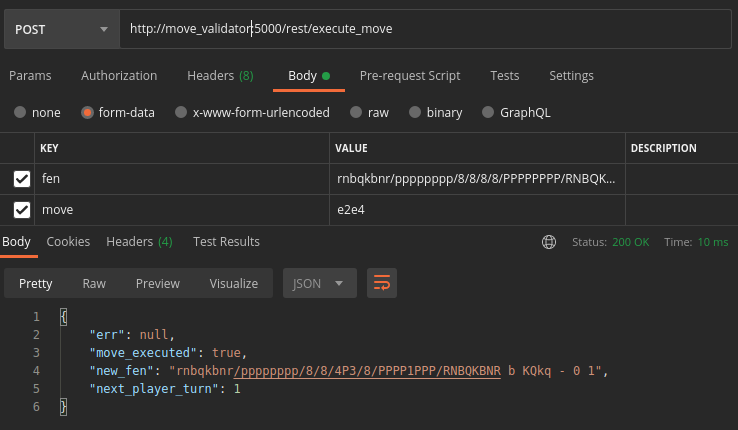
\includegraphics{images/ATC_movevalidator_execute_move.png}
\caption{MoveValidator: Beispiel Request zur Ausführung eines Zuges auf
einem gegebenen Schachbrett \label{ATC_movevalidator_execute_move}}
\end{figure}

Der Backend-Service fragt ein neues Spiel an oder übergibt einen
Schachzug inkl. des aktuellen Spielbrett-Aufbaus an den
Service.\ref{ATC_movevalidator_execute_move} Der Response wird dann vom
Backend in der Datenbank gespeichert und weiter an die Client-Devices
verteilt.

\begin{longtable}[]{@{}lccr@{}}
\caption{MoveValidator-Service \gls{api} Overview
\label{finalfeaturesatc}}\tabularnewline
\toprule
MoveValidator-Function & \gls{api}-Route & Method &
Form-Data\tabularnewline
\midrule
\endfirsthead
\toprule
MoveValidator-Function & \gls{api}-Route & Method &
Form-Data\tabularnewline
\midrule
\endhead
Check Move & /rest/check\_move & POST & fen, move, player\tabularnewline
Execute Move & /rest/execute\_move & POST & fen, move\tabularnewline
Validate Board & /rest/validate\_board & POST & fen\tabularnewline
Init Board & /rest/init\_board & GET &\tabularnewline
\bottomrule
\end{longtable}

Allgemein geschieht die Kommunikation über vier \gls{api} Calls, welche
vom MoveValidator-Service angeboten werden \ref{finalfeaturesatc}. Als
erstes wird vom Backend der \passthrough{\lstinline!/rest/init\_board!}
Request verwendet, welcher ein neues Spielbrett in der \gls{fen}
Notation zurückgibt, welches zum Start der Partie verwendet wird.
Allgemein arbeitet wurde das komplette System so umgesetzt, dass dieses
mit einem Spielfeld in einer Zeichenketten representation arbeitet. Dies
hat den Vorteil, dass die Spielfeld-Notation leicht angepasst werden
kann. Mit diesem Design ist es möglich, auch andere Spielarten im System
zu implementieren, da nur an dieser Stelle die initialen Spielfelder
generiert werden und Züge der Spieler validiert werden müssen.

Die \gls{fen} Notation ist universal und kann jede Brettstellung
darstellen. Auch enthält diese nicht nur die Figur Stellungen, sondern
auch weitere Informationen, wie die aktuelle Nummer des Zuges oder
welcher Spieler gerade an der Reihe ist. Diese werden dann in der
\gls{xfen} Notation angegeben, bei der zusätzlich zu der Brettstellung
auch noch die weiteren Informationen angehängt werden \ref{fenxfen}.

\begin{longtable}[]{@{}lr@{}}
\caption{Vergleich \gls{fen} - \gls{xfen}
\label{fenxfen}}\tabularnewline
\toprule
FEN-TYPE & FEN-String\tabularnewline
\midrule
\endfirsthead
\toprule
FEN-TYPE & FEN-String\tabularnewline
\midrule
\endhead
FEN & rnbqkbnr/pp1ppppp/8/2p5/4P3/5N2/PPPP1PPP/RNBQKB1R\tabularnewline
X-FEN & rnbqkbnr/pp1ppppp/8/2p5/4P3/5N2/PPPP1PPP/RNBQKB1R b KQkq - 1
2\tabularnewline
SCHEMA & Board Player-Color Rochade En-Passant Halfturn
Turn-Number\tabularnewline
\bottomrule
\end{longtable}

Alle gängigen Schachprogramme und Bibliotheken unterstützen das Laden
von Spielbrettern in der \gls{fen} bzw \gls{xfen} Schreibweise, ebenso
die für den MoveValidator Service verwendete Python-Chess Bibliothek
\cite{pythonchesslib}. Diese unterstützt zusätzlich die Generierung
der für den Benutzer möglichen Schachzügen, welche auf dem aktuellen
Brett möglich sind.

Diese Liste wird vom System dazu verwendet, um sicherzustellen, dass der
Benutzer nur gültige Züge tätigen kann. Diese Funktion lässt sich
zusätzliche abschalten, falls das Spiel nicht nach den allgemeinen
Schachregeln verlaufen soll. Bei der Generierung der möglichen
Schachzüge muss zwischen den Legal-Moves und den Pseudo-Legal
Schachzügen unterschieden werden. Die Legal-Moves beinhalten nur die
nach den Schachregeln möglichen Zügen, welche von Figuren des Spielers
ausgeführt werden können. Die Pseudo-Legal Schachzüge sind alle
Schachzüge, welche von den Figuren auf dem aktuellen Schachbrett möglich
sind; darin sind unter anderem auch alle anderen Figur-Züge enthalten,
solange der König des aktuellen Spielers sich aktuell auf dem
Schachbrett befindet.

Wenn ein Spieler an der Reihe ist und einen Zug getätigt hat, wird sein
getätigter Zug mittels der \passthrough{\lstinline!/rest/check\_move!}
\gls{api} überprüft und festgestellt, ob dieser gemäß der Legal-Moves
durchführbar war. Ist dies der Fall, wird der Zug auf dem
online-Spielbrett angewendet. Dies geschieht durch die
\passthrough{\lstinline!/rest/execute\_move!} \gls{api}. Diese führt den
Zug aus, ermittelt anschließend das neue Spielbrett und überprüft
zusätzlich, ob das Spiel gewonnen oder verloren wurde.

Hat der Benutzer jedoch einen ungültigen Zug ausgeführt, wird dieser vom
System storniert und der Client des Benutzers stellt den Zustand des
Spielbretts vor dem getätigten Zug wieder her. Danach hat der Benutzer
die Möglichkeit einen alternativen Zug auszuführen.

\hypertarget{service-webclient}{%
\section{Service: Webclient}\label{service-webclient}}

\begin{figure}
\centering
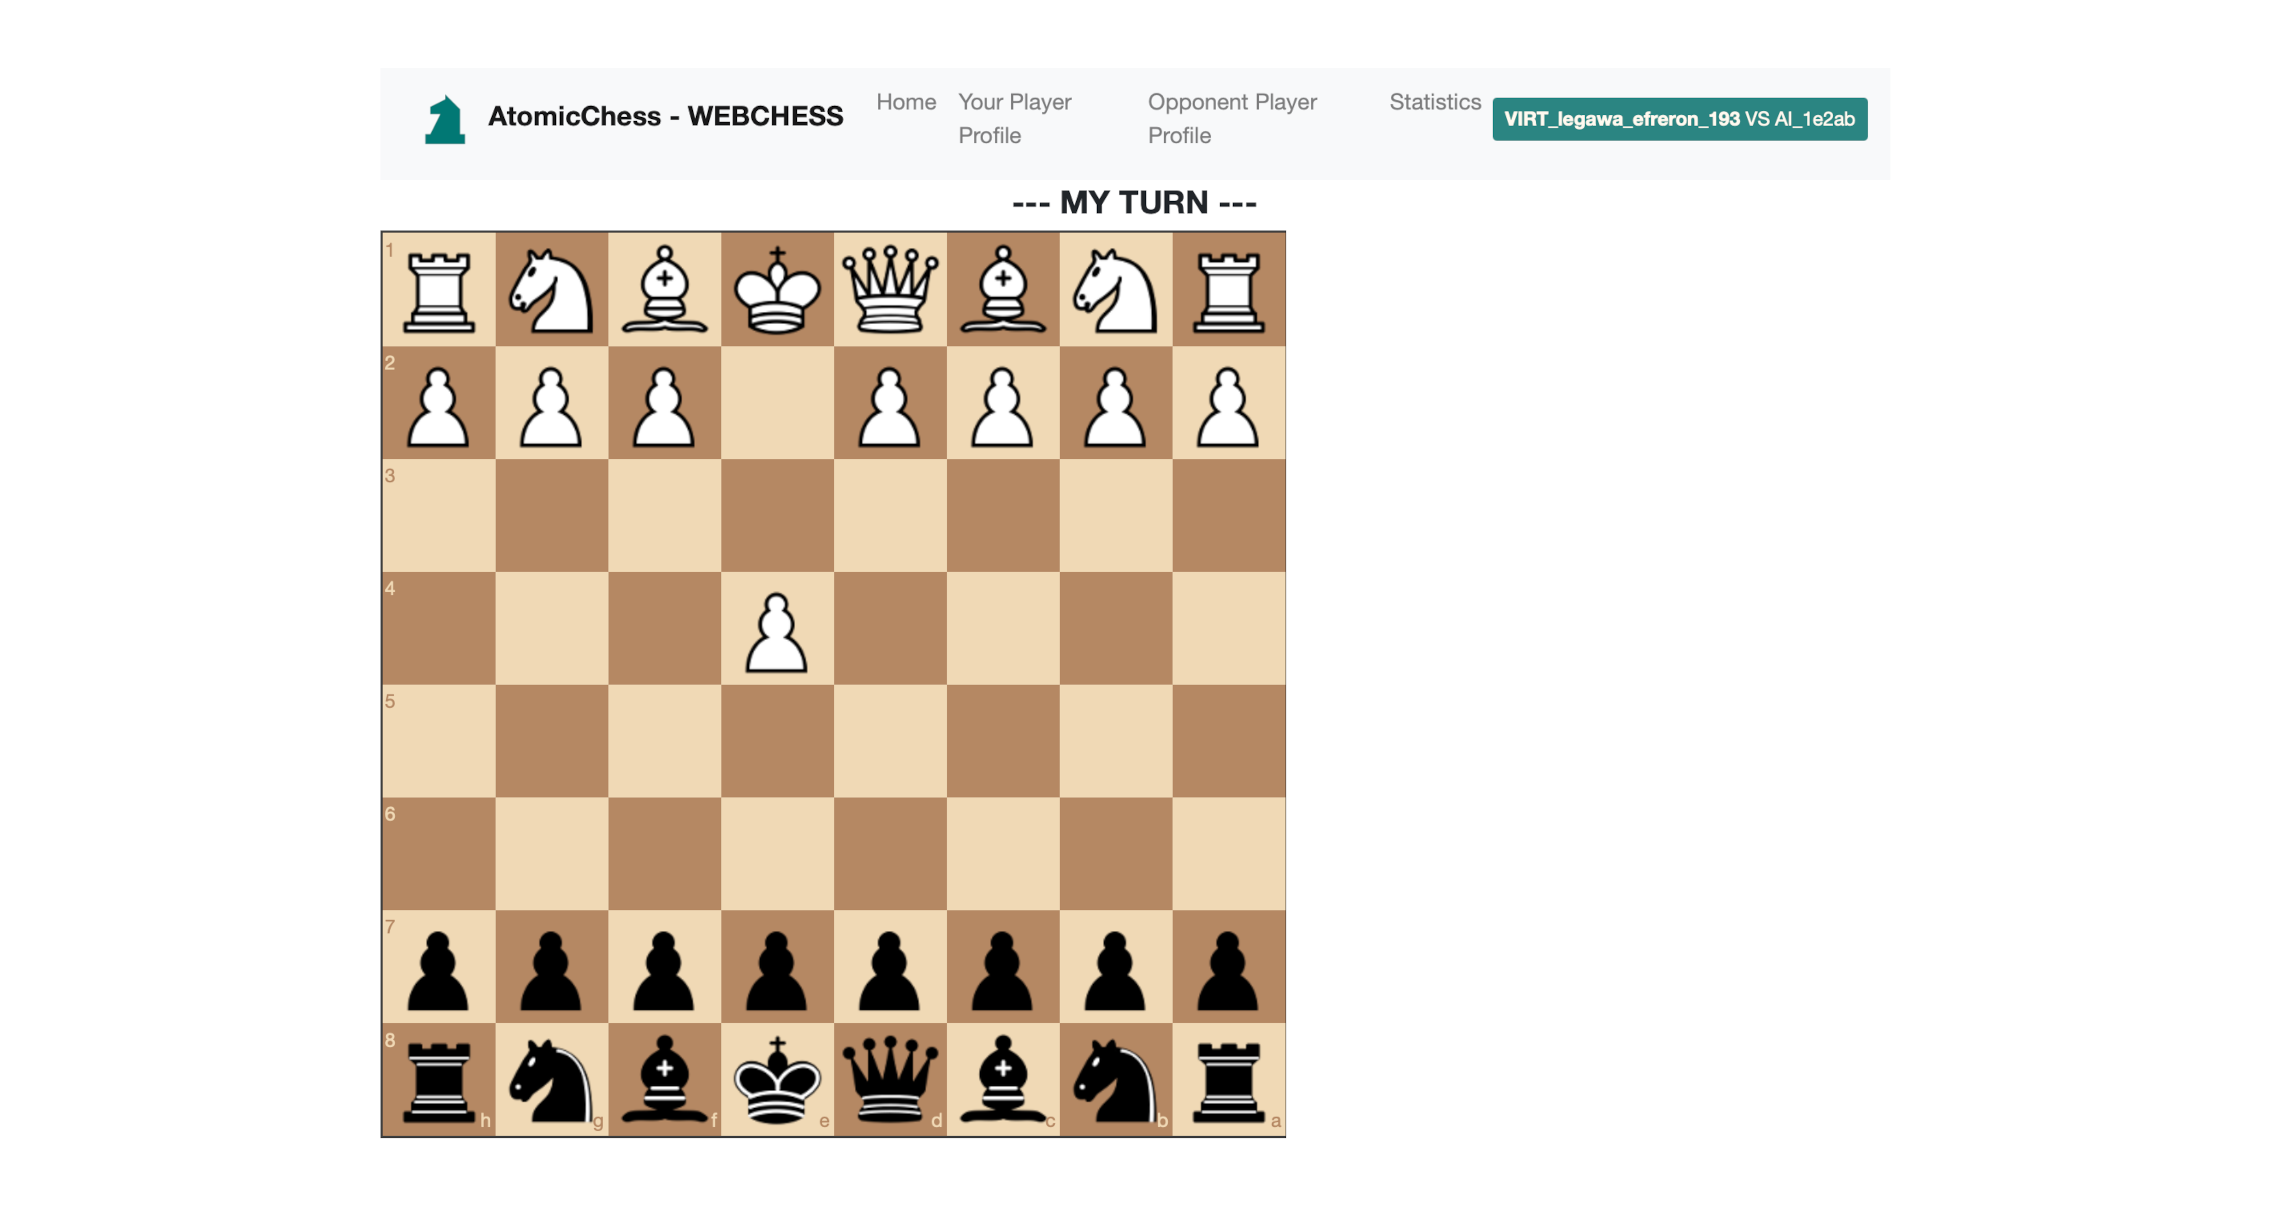
\includegraphics{images/ATC_webclient.png}
\caption{Webclient: Spielansicht \label{ATC_webclient}}
\end{figure}

Der Webclient wurde primär dazu entwickelt, um das System während der
Entwicklung zu testen. Dieser simuliert einen autonomen Schachtisch und
verwendet dabei die gleichen \gls{http} Requests. Um das zu ermöglichen
wurde dieser vollständig in \gls{js} umgesetzt im Zusammenspiel mit
\gls{html} und \gls{css} und ist somit komplett im Browser ausführbar.

Ausgeliefert werden die statischen Dateien zur Einfachheit durch den
Backend-Service; es wurde kein gesonderter Frontend-Service angelegt.
Durch die Implementierung des Webclienten in \gls{js} ist dieser sogar
lokal über einen Browser ausführbar, ohne dass die benötigten Dateien
über einen Webserver ausgeliefert werden müssen.

Zusätzlich zu dem verwendeten Vanilla-\gls{js} wurde
\passthrough{\lstinline!jQuery!}\cite{jquery} als zusätzliche
\gls{js} Bibliothek verwendet, welches eine Manipulation der \gls{html}
Elemente stark vereinfacht. Diese bietet insbesondere einfach zu
nutzende \gls{http}-Request Funktionen bzw. \gls{ajax} an, welche für
die Kommunikation mit dem Backen-Service verwendet werden. Diese werden
im Hintergrund eingesetzt, sodass der Webclient automatisch den neuen
Spielzustand dem Benutzer anzeigt. Dies geschieht mittels
\passthrough{\lstinline!polling!}, bei dem der Webbrowser in zyklischen
Abständen die aktuellen Spiel-Informationen vom Backen-Service abfragt.
Diese Methode wurde verwendet, um eine maximale Kompatibilität mit
verschiedensten gegebenenfalls älteren Web-Browsern sicherzustellen.
Eine moderne alternative ist die Verwendung von Web-Sockets, bei welcher
der Web-Browser eine direkte \gls{tcp}-Verbindung zum Webserver (in
diesem Fall der Backend-Service) aufnehmen und so eine direkte
Kommunikation stattfinden kann ohne Verwendung der
\passthrough{\lstinline!polling!}-Methode.

Der Hauptanwendungsfall des Webclienten \ref{ATC_webclient} während der
Entwicklung ist es, weitere Spieler zu simulieren und so ein Spiel mit
nur einem autonomen Schachtisch testen zu können. Durch den Webclient
ist zusätzliche möglich, gezielt Spiele und Spielzüge zu simulieren.
Hierzu gehören vor allem Sonderzüge wie die Rochade oder der En-Passant
Zug. Auch können durch den Webclient ungültige Züge simuliert werden,
welche durch die Verwendete Schach-\gls{ai} nicht getätigt werden.

Während der Implementierung wurde der Webclient weiter ausgebaut und es
wurde weitere Eigenschaften ergänzt. Dazu zählt zum einen eine Übersicht
über vergangene und aktuell laufende Spiele. In dieser können Spiele Zug
um Zug nachvollzogen werden und weitere Information über den Spielstatus
angezeigt werden.\ref{ATC_statistics} Auch ist es möglich, aktuell
laufende Spiele in Echtzeit anzeigen zu lassen; somit wurde eine
Livestream-Funktionalität implementiert.

\begin{figure}
\centering
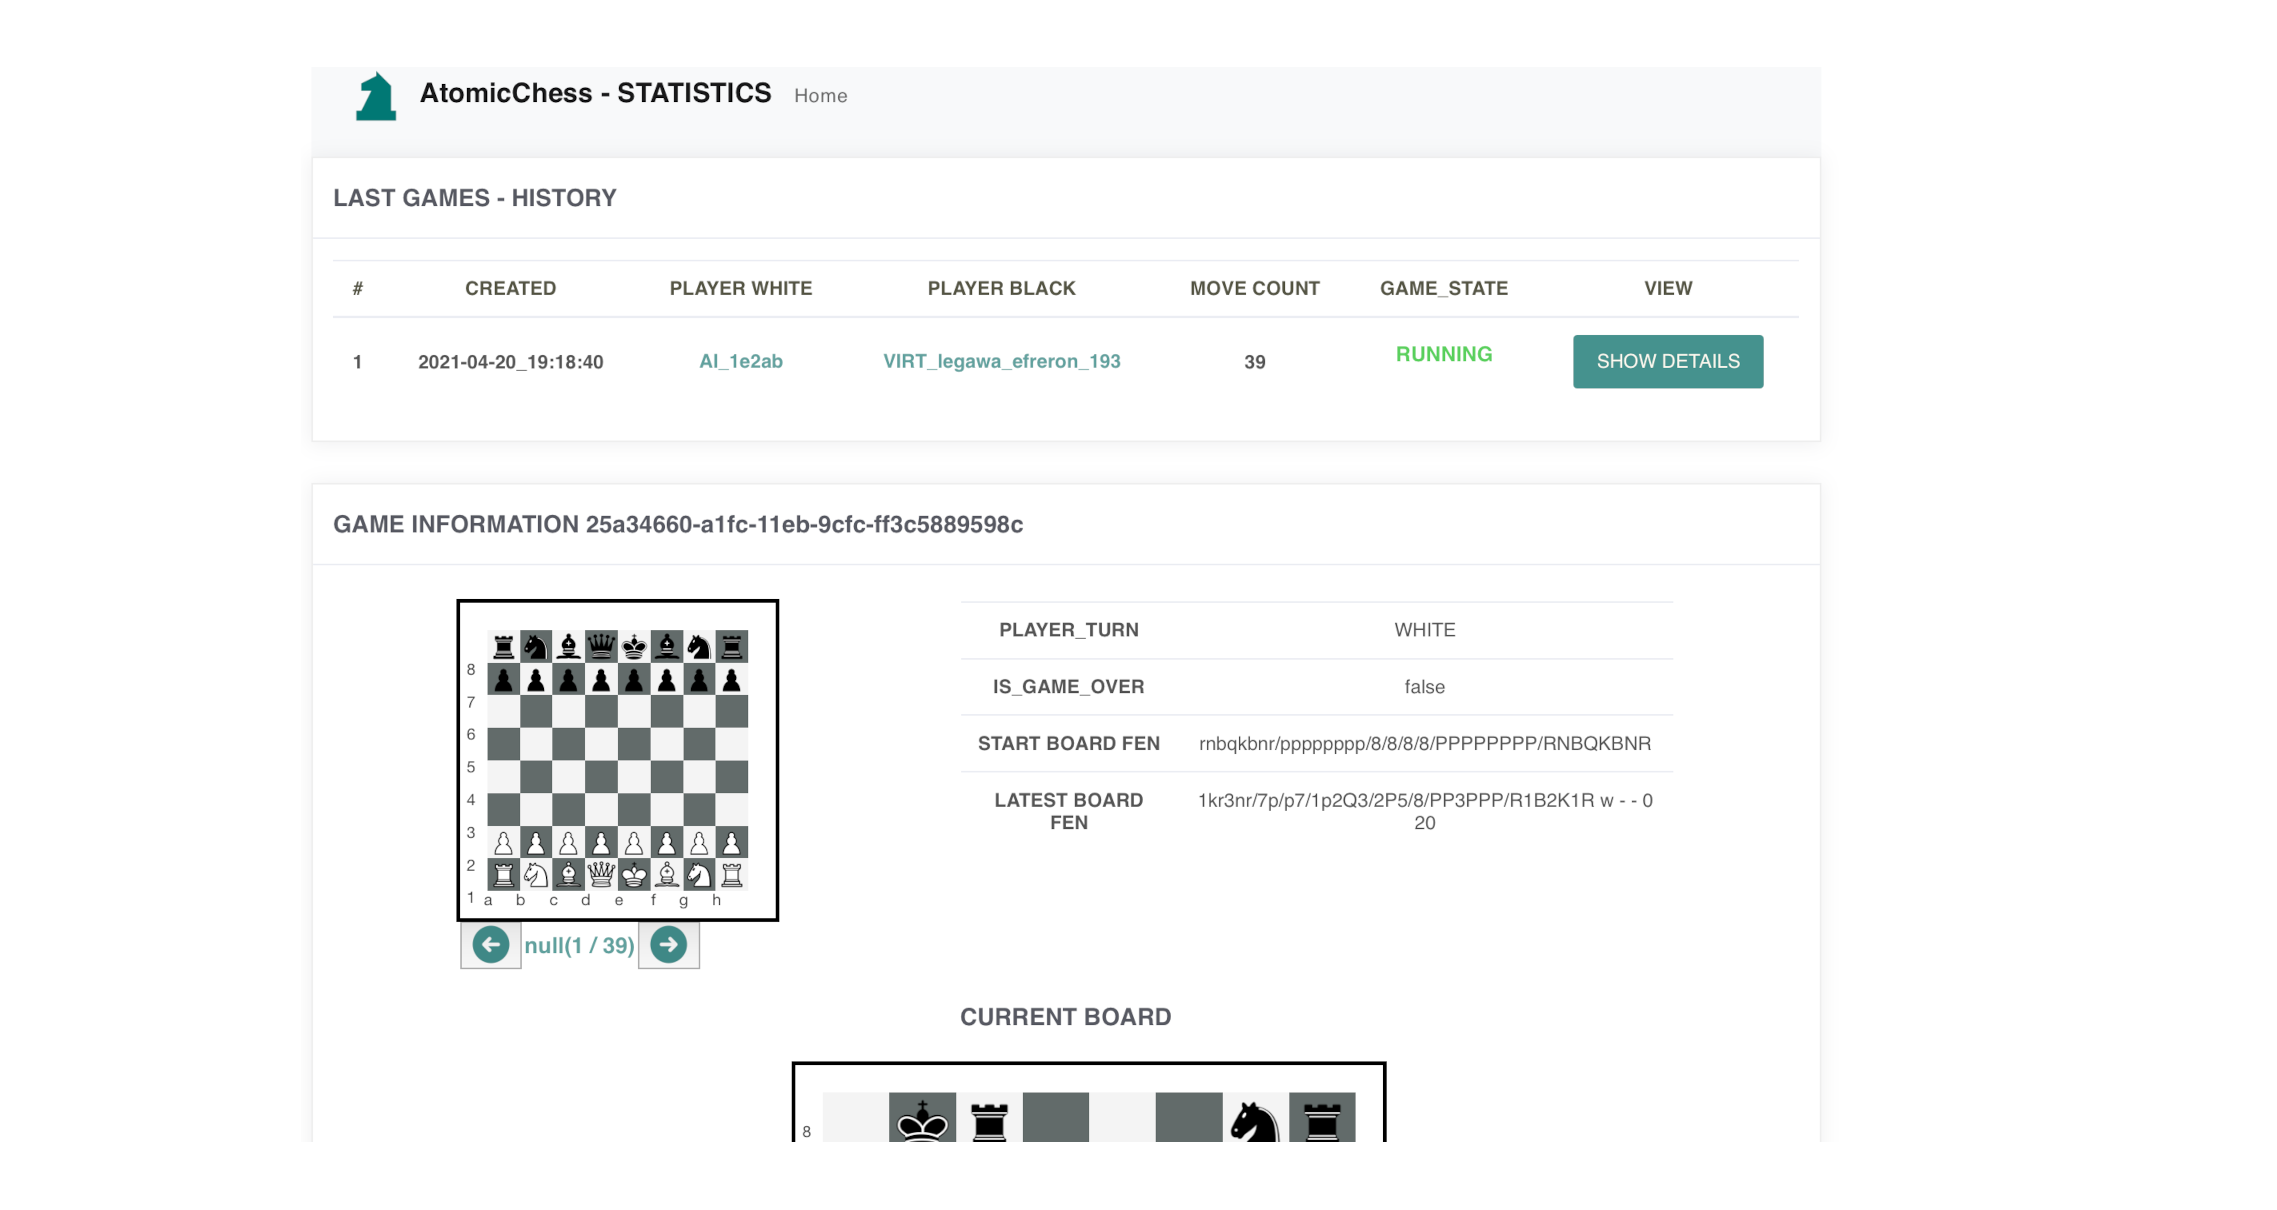
\includegraphics{images/ATC_statistics.png}
\caption{Webclient: Statistiken \label{ATC_statistics}}
\end{figure}

\hypertarget{service-autoplayer}{%
\section{Service: AutoPlayer}\label{service-autoplayer}}

Der AutoPlayer-Service stellt den Computerspieler bereit.

Jede Service-Instanz stellt einen virtuellen Spieler bereit, welcher die
gleichen Schnittstellen wie der Webclient oder der autonome Schachtisch
verwendet. Die einzige Änderung an den verwendeten \gls{rest}-Calls ist
der Login-Request. Hier wird das \passthrough{\lstinline!playertype!}
Flag gesetzt welches den Spieler als Computerspieler gegenüber dem
System authentifiziert. Daraus resultierend wird dieser während des
Matchmaking-Prozesses erst für ein Match ausgewählt, wenn keine anderen
menschlichen Spieler mehr zur Verfügung stehen. Dieser digitale
Gegenspieler ist vom Typ Webclient oder autonomer Schachtisch. Dieser
Prozess gewährleistet zudem, dass immer zuerst die menschlichen Spieler
ein Spiel beginnen und die digitalen nur Alternativen darstellen.

Eine weitere Modifikation ist die Verwendung einer Schach-\gls{ai}, da
dieser Service als Computerspieler agieren soll. Hierzu kam die
Open-Source Chess Engine Stockfish\cite{stockfish} in der Version 11
zum Einsatz. Die Stockfish-Engine bietet noch weitere Features, als nur
die nächstbesten Züge zu einem gegebenen Schachbrett zu ermitteln.

Die AutoPlayer-Instanz kommuniziert über das \gls{uci}
Protokoll\cite{uciprotocol} mit der Engine. Dieses Protokoll wird in
der Regel von Schach-Engines verwendet, um mit einer \gls{gui} zu
kommunizieren.

Um das aktuelle Spielbrett in der Engine zu setzten wird dieses in der
\gls{xfen} Notation mit dem Präfix
\passthrough{\lstinline!position fen!} als Klartext an die Engine
übergeben und sendet daraufhin eine List möglicher Züge zurück. Der
erste Index dieser Liste ist dabei der am besten bewerteten Zug der
Engine.

Im Kontext des AutoPlayer-Service wird der Engine nur das aktuelle
Spielbrett übermittelt und der nächstbeste Zug auslesen. Dies wird
ausgeführt, wenn der AutoPlayer am Zug ist. Nachdem die Engine einen
passenden Zug gefunden hat, wird das Ergebnis über den
\passthrough{\lstinline!make\_move!} (+rest)-\gls{api} Call übermittelt.

Wenn das Match beendet wird, beendet sich auch die Service-Instanz.
Diese wird jedoch wieder gestartet, wenn die Anzahl der zur Verfügung
stehenden Computerspieler unter einen definierten Wert fallen. Somit ist
dafür gesorgt, dass das System nicht mit ungenutzten
AutoPlayer-Instanzen gebremst wird. Diese Anzahl \ref{ai_player_count}
ist in der Konfiguration des Backend-Service frei wählbar und kann je
nach zu erwarteten Aufkommen angepasst werden.

Allgemein skaliert das System durch diese Art der Ressourcenverwaltung
auch auf kleinen Systemen sehr flexibel. Durch die Art der
Implementierung, dass sich der AutoPlayer-Service wie ein normaler
Spieler verhält, sind auch andere Arten des Computerspieler möglich. So
ist es zum Beispiel möglich, die Spielstärke je Spieler anzupassen oder
einen Computerspieler zu erstellen, welcher nur zufällige Züge zieht.

Ein weiterer Anwendungsfall für den AutoPlayer-Service, ist das Testen
des weiteren Systems insbesondere des Backend-Service. Durch das
Erstellen eines Spiels mit zwei AutoPlayer-Instanzen, können
automatisierte Schachpartien ausgeführt werden, um die
Funktionsfähigkeit des restlichen Systems zu testen. Diese Feature wurde
insbesondere bei der Entwicklung des Webclient und der
Steuerungssoftware für den autonomen Schachtisch verwendet.

\hypertarget{embedded-system-software}{%
\chapter{Embedded System Software}\label{embedded-system-software}}

\begin{itemize}
\tightlist
\item
  Hauptsoftware zur Steuerung der Elektrik/Mechanik
\item
  Kommunikation mit dem Cloud-Server
\end{itemize}

\hypertarget{ablaufdiagramm}{%
\section{Ablaufdiagramm}\label{ablaufdiagramm}}

Nach dem Start der Controller-Software folgt diese einem Fest
vorgegebenen Ablauf \ref{ATC_gameclient_statemachiene}. Dieser wird
mittels einer State-Machine in der Controller-Software abgebildet.
Nachdem die Software gestartet ist, wird zuerst eine Verbindung mit dem
Cloud-Server aufgenommen. Da der Tisch eine Art Thin-Client darstellt,
bei dem die eigentliche Spiellogik auf dem Server ausgeführt wird, muss
die Controller-Software nur das vom Server vorgegebene Schachfeld
mittels der Mechanik synchronisieren und entsprechende Schachzüge des
Benutzers an diesen übermitteln.

\begin{figure}
\centering
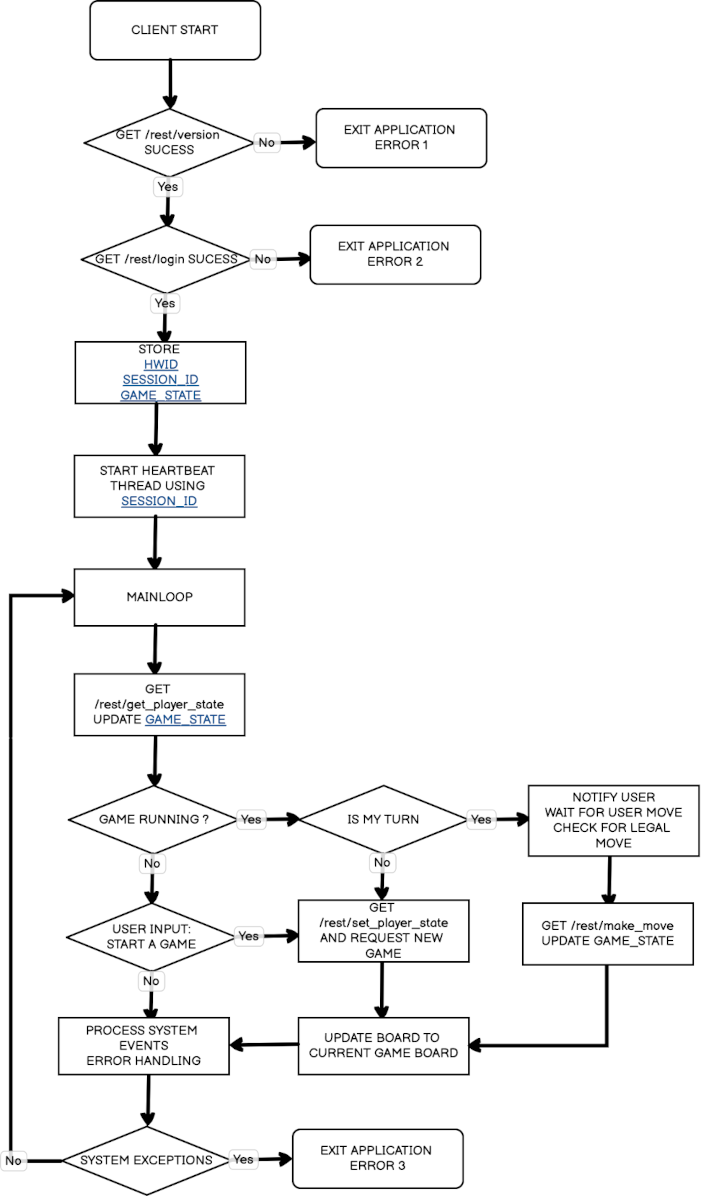
\includegraphics{images/ATC_gameclient_statemachiene.png}
\caption{Embedded System Software: Ablaufdiagramm
\label{ATC_gameclient_statemachiene}}
\end{figure}

Nach erfolgreicher Anmeldung am Cloud-Server, kann der Benutzer ein
Spiel starten, welches lediglich zu einem entsprechenden Request an den
Server führt. Die nachfolgende Dauerschleife überprüft, ob ein Spiel
gestartet wurde. Dazu wird in zyklischen Intervallen die
\passthrough{\lstinline!/rest/get\_playerstate!} \gls{api} aufgerufen.
Diese stellt Informationen ob und in welchem Status sich das Spiel für
den anfragenden Client befindet.

Wurde das Spiel gerade erst gestartet, beginnt die Sync-Phase. Bei
dieser müssen beide Clients, die Figuren in die vorgegeben
Ausgangsstellung bringen und dies bestätigen. Erst dann gilt das Spiel
für den Server als begonnen und der aktive Spieler wird ausgewählt. Ist
der Client am Zug, wartet dieser auf einen Zug in Form einer
Benutzereingabe. Welches entweder durch manuelles Eintippen des
Schachzugs über die \gls{gui} geschieht oder über eine manuelle Bewegung
der Figuren. Auch hier hat der Client keine Informationen darüber ob der
getätigte Zug gültig ist. Die Zuginformationen werden über die
entsprechende \gls{api} Route \passthrough{\lstinline!/rest/make\_move!}
an den Server übermittelt, welcher diesen Zug auf dem Schachbrett
ausführt. Wenn der Zug ungültig ist, muss der Client den Benutzer
informieren, diesen Rückgängig zu machen. Ist der Zug jedoch gültig, wir
dieser vom Server an den anderen Client übermittelt und dieser muss
anschließend wie beider Sync-Phase das Spielbrett aufbauen.

Nach einem Abbruch oder einem Gewinn oder Verlust des Spiels, wartet der
Client wieder, bis ein neues Spiel vom Server aus gestartet wird, oder
der Benutzer manuell ein Spiel startet. Dieser Zyklus wird dauerhaft
ausgeführt. Der Client bietet jedoch noch weitere
Einstellungsmöglichkeiten für den Benutzer über die \gls{gui} an. Diese
Benutzer-Events werden separat verarbeitet und sind vom Spielablauf
getrennt. Hierzu zählen unter anderem der Kalibrierungs-Dialog sowie
eine Informationsansicht über den aktuellen Status des Systems.

\hypertarget{figur-bewegungspfadberechnung}{%
\section{Figur
Bewegungspfadberechnung}\label{figur-bewegungspfadberechnung}}

Nach dem Start der Software wird durch das Abscannen jedes einzelnen
Feldes die Anzahl und Typen der Figuren ermittelt. Dies stellt sicher,
dass sich die Erforderliche Anzahl der Figuren beim Systemstart auf dem
Spielbrett befinden, ansonsten in ein Start des Programms nicht möglich.

Während der Sync-Phase muss die Software das vorgegebene Schachfeld
herstellen. Dazu hält die Software den aktuellen Brett-Zustand vor und
vergleicht diese mit dem Ziel-Schachbrett. Durch einen Vergleich dieser
können die sich geänderten Figuren lokalisiert werden. Dadurch dass
immer Ziel und Aktuelles-Spielbrett miteinander verglichen werden,
können mehrere Züge auf einmal durchgeführt werden. Hierbei ist es auch
möglich auf Spielbrett in einem Zustand X, wieder die Ausgangsposition
herstellen zu können. Somit kann ein beliebiges Spielfeld vorgegeben
werden, welches der Tisch dementsprechend aufbaut.

Um dies zu ermöglichen, wird aus der Vergleich der beiden Spielbretter
eine Differenz in Form einer Liste gebildet. In dieser sind alle
Änderungen eines einzelnen Feldes vermerkt. Eine Änderung besteht aus
der Figur, welche sich aktuell auf dem Brett befindet, und dem
Ziel-Zustand.

\begin{lstlisting}[language={C++}]
//ChessBoard.cpp
std::vector<ChessBoard::FigureFieldPair>
ChessBoard::compareBoards(ChessPiece::FIGURE *_board_a, ChessPiece::FIGURE *_board_b, bool _include_park_pos) {
    std::vector<ChessBoard::FigureFieldPair> diff_list;
    ChessPiece::FIGURE *board_current = get_board_pointer(ChessBoard::BOARD_TPYE::REAL_BOARD);
    ChessPiece::FIGURE *board_target = get_board_pointer(ChessBoard::BOARD_TPYE::TARGET_BOARD);
    //..
    //NOW CHECK BOARD DIFFERENCES
    for (int i = ChessField::field2Index(ChessField::CHESS_FILEDS::CHESS_FIELD_A1);
         i < ChessField::field2Index(ChessField::CHESS_FILEDS::CHESS_FIELD_PARK_POSTION_WHITE_1); i++) {
        ChessPiece::FIGURE tmp_curr = getFigureOnField(board_current, ChessField::Index2Field(i));
        ChessPiece::FIGURE tmp_target = getFigureOnField(board_target, ChessField::Index2Field(i));
        //CHECK IF EQUAL FIGURES
        if (ChessPiece::compareFigures(tmp_curr, tmp_target)) {
            continue;
        }
        ChessBoard::FigureFieldPair tmp;
        tmp.field_curr = ChessBoard::FigureField(ChessField::Index2Field(i), tmp_curr);
        tmp.field_target = ChessBoard::FigureField(ChessField::Index2Field(i), tmp_target);
        tmp.processed = false;
        diff_list.push_back(tmp);
    }
    return diff_list;
}
\end{lstlisting}

Aus dieser Liste können anschließend einzelne Figur-Bewegungen
abgeleitet werden. Dazu wird zu einer Änderung des Start-Feldes in der
Liste ein weiteres Listenelement gesucht, bei welchem die Änderung im
Zielfeld liegt. Somit kann Start- und Zielfeld für eine Figur bestimmt
werden. Anzumerken ist, dass die errechneten Züge nicht die logischsten
oder kürzesten darstellen müssen. Da hier die Reihenfolge der Änderungen
nach vorkommen in der Liste entscheidend ist. Somit entsteht eine
weitere Liste an Feld-Operationen, bei denen Figuren hinzugefügt,
bewegt, entfernt werden können.

\begin{itemize}
\tightlist
\item
  überschüssige Figuren entfernen

  \begin{itemize}
  \tightlist
  \item
    wenn allgemein zu viele Figuren auf dem Feld sind
  \item
    wenn bei dem auszuführenden Zug eine Figur geschlagen wird
  \end{itemize}
\item
  möglichen Zug ausführen

  \begin{itemize}
  \tightlist
  \item
    falls Figuren fehlen diese hinzufügen
  \item
    sonst Figur an Zielposition bewegen
  \end{itemize}
\item
  Figur fehlt

  \begin{itemize}
  \tightlist
  \item
    Figur aus Park-Position auf das Spielbrett holen
  \end{itemize}
\end{itemize}

Dieser Vorgang wird rekursiv solange ausgeführt bis es keine Änderungen
auf dem Spielbrett mehr gibt. Der rekursive Ansatz ist notwendig, da
nicht alle Figuren ihren Bestimmungsort einnehmen können, wenn diese
noch von einer anderen Figur belegt sind. Diese muss zuerst auf deren
Ziel-Feld geschoben werden.

Aus den Start und Ziel-Feldern werden im letzten Schritt-Wegpunkte
\ref{ATC_FigureMoveAlgorithm} generiert. Diese beschreiben den Weg,
welchen die Figur von Start zum Zielfeld ablaufen muss. Das Spielbrett
wurde so designt, dass zwischen jeder Figur auf dem Feld immer eine
weitere Figur Platz hat. Somit ist es möglich, dass die sich bewegenden
Figuren zwischen zwei auf ihren Feldern stehenden hindurchbewegt werden
können. Der Algorithmus berechnet genau diese Wegpunkte. Nachdem die
Figur aus der Mitte des Feldes und an den Rand dieses Bewegt wurde, kann
die Figur ungehindert zwischen den anderen vorbei bewegt werden. Die
Figur wird anschließend in Richtung der X-Achse auf die Höhe des
Zielfeldes bewegt um darauffolgend auf der Y-Achse an die Kante des
Zielfeldes bewegt zu werden. Der letzte Wegpunkt liegt im inneren des
Zielfelds, sodass sich die Figur in der Mitte diesem befindet.

\begin{figure}
\centering
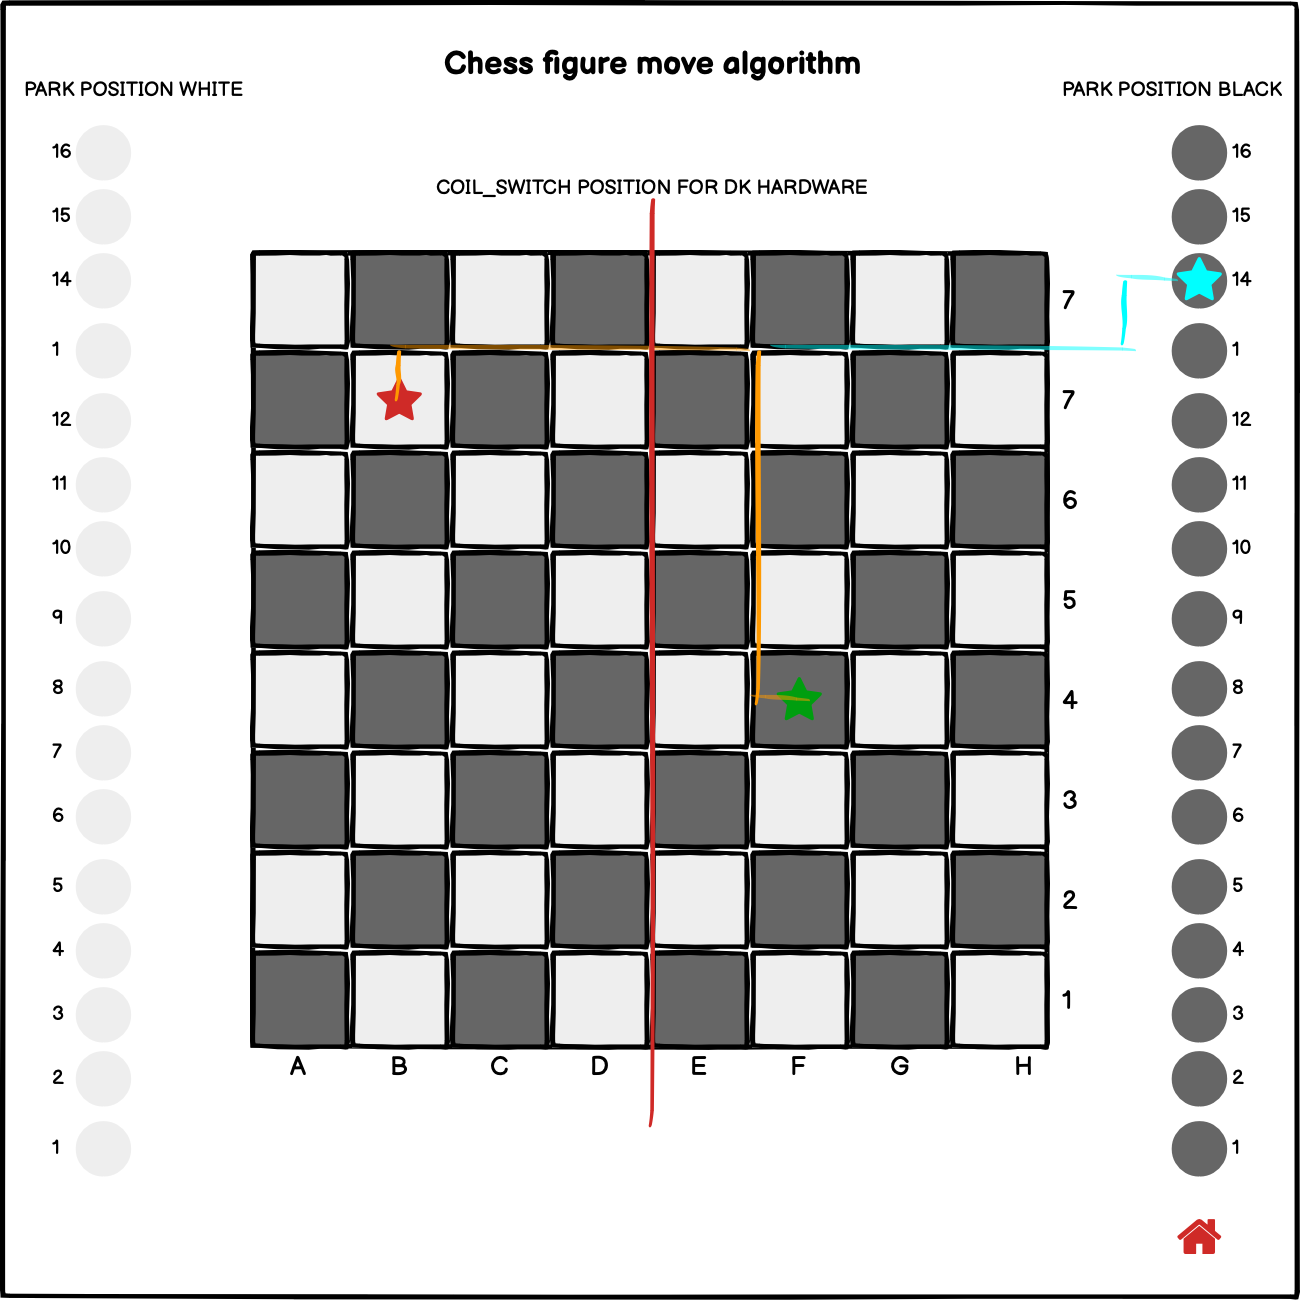
\includegraphics{images/ATC_FigureMoveAlgorithm.png}
\caption{Embedded System Software: Figur Wegpunkte
\label{ATC_FigureMoveAlgorithm}}
\end{figure}

Anzumerken ist, dass dieser Algorithmus nicht weiter optimiert wurde,
somit führen die Figuren auch eine Zick-Zack-Bewegung aus auch wenn das
Zielfeld direkt neben dem Start-Feld liegt.

\hypertarget{schachfeld-scan-algorithmus-zur-erkennung-von-schachzuxfcgen}{%
\section{Schachfeld Scan Algorithmus zur Erkennung von
Schachzügen}\label{schachfeld-scan-algorithmus-zur-erkennung-von-schachzuxfcgen}}

Ein weiterer wichtiger Teil der Controller-Software ist die Erfassung,
der Schachzüge welche vom Benutzer getätigt wurden. Das System bietet
dem Benutzer hier zwei Möglichkeiten, welche im Folgenden erläutert
werden. Über das \gls{ui} des autonomen Schachtischs kann der Benutzer,
wenn dieser am Zug ist, manuell eingegeben werden. Hierbei wird das
Start- und Ziel-Feld angegeben, woraus das System automatisch den
gewünschten zug ermittelt. Dies ist jedoch bei einer Schachpartie nicht
praktikabel. Der Benutzer muss eine Möglichkeit haben, die Schachfiguren
händisch bewegen zu können. Das System muss aus den geänderten Figuren
den getätigten Schachzu ermitteln könnnen.

Da das Schachbrett in beiden Revisions-Varianten über keine Sensoren
unter den einzelnen Schachfelder verfügt, wurde der existierenden
\gls{nfc} Scanner verwendet. Mit dem ist es möglich gezielt Figuren auf
zuvor bestimmten Feldern zu ermitteln. Der Nachteil dieser Methode ist
die Wartezeit, welche aufgrund des Scan-Prozesses nötig ist. Ein Scan
aller 64 Felder ist nicht praktikabel, da jeder Scan und der Bewegung
der Mechanik ca 3 Sekunden benötigt. Zusätzlich verlängert sich die
Scandauer durch ein leeres Schachfeld, da der Scanner mehrere Versuche
unternimmt ein gültiges \gls{nfc} Tag zu erkennen.

Somit muss mittels eines Algoritmus \ref{ATC_ChessMoveAlgorithm}
entschieden werden, welches Felder als mögliche Kandidaten in Fragen
kommen. Hinweise auf diese Felder bietet der aktuelle Spiel-Status,
welche vom System über den Cloud-Service abgefragt wird. Dieser liefert
nicht nur das aktuelle Schachbrett, sondern auch die möglichen
Schachzüge, welche vom Benutzer ausgeführt werden können.

\begin{figure}
\centering
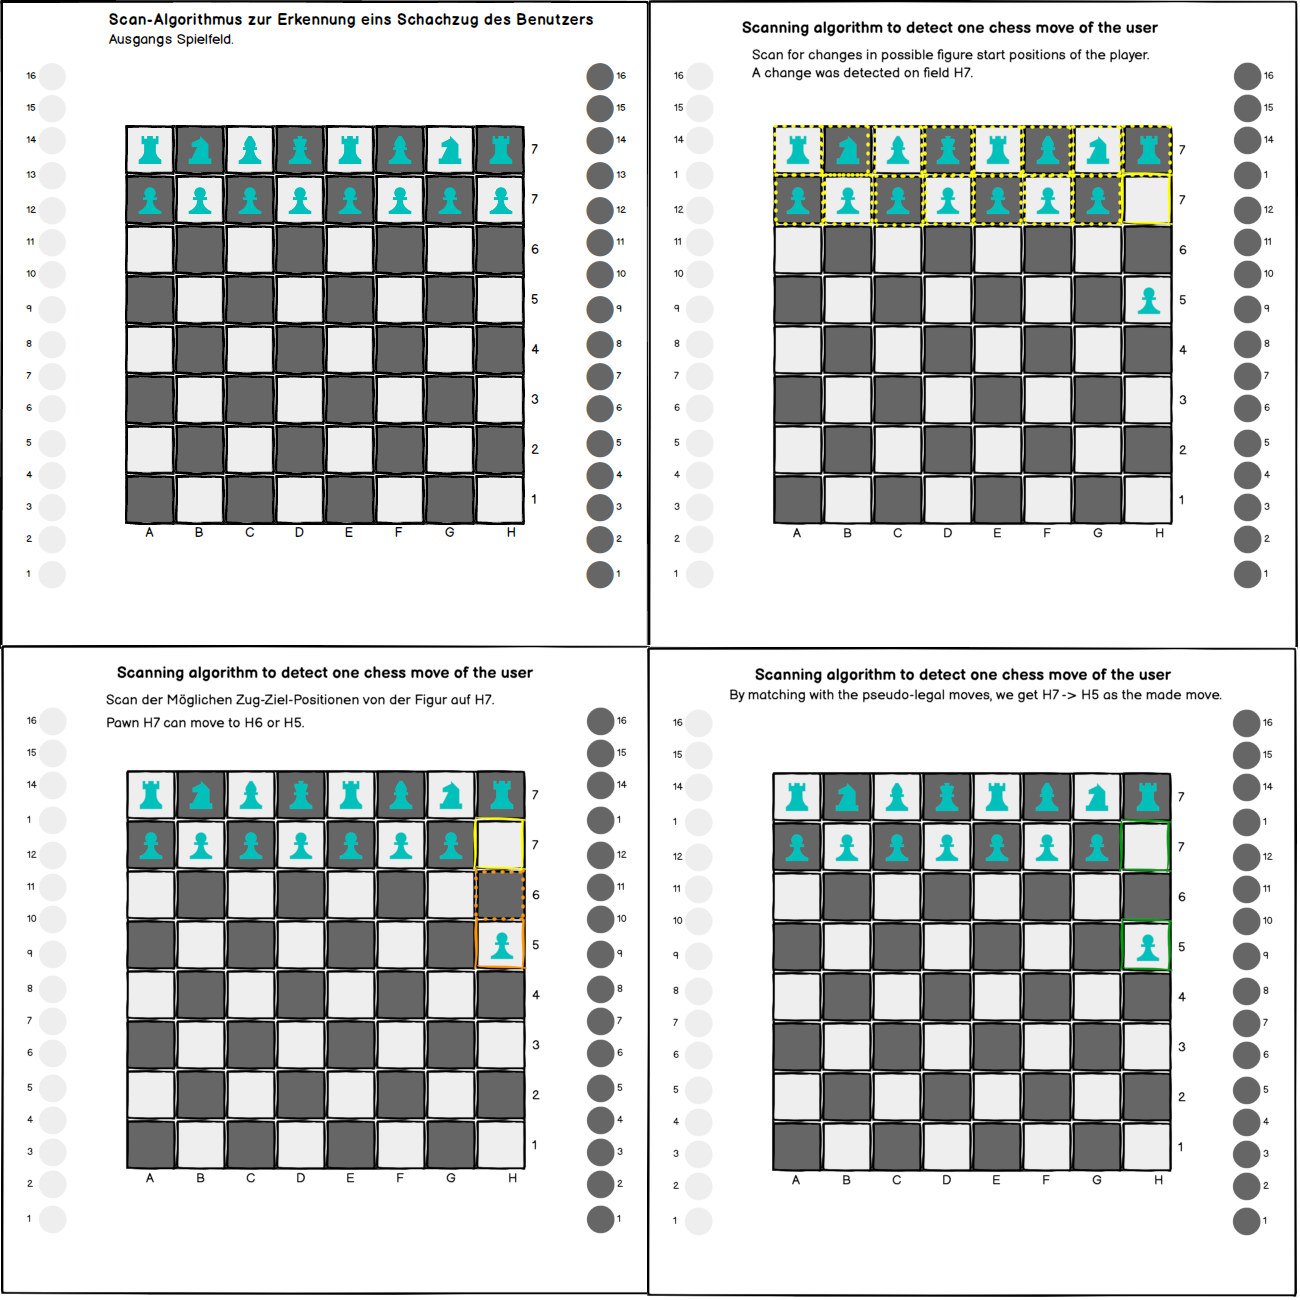
\includegraphics{images/ATC_ChessMoveAlgorithm.png}
\caption{Embedded System Software: Schachfeld Scan Algorithmus Ablauf
\label{ATC_ChessMoveAlgorithm}}
\end{figure}

Durch diese Auflistung an mögliche Zügen, wird anschließend eine Liste
mit den mögliche Start-Feldern der Figuren erstellt. Anhand dieser Liste
werden die Felder mittels des \gls{nfc} Moduls auf Veränderungen
überprüft. Stellt das System eine Änderung fest, wird ermittelt, auf
welche Felder die Figur auf dem Feld ziehen kann. Anschließend werden
alle Ziel-Feld Positionen der Figur abgescannt, bis auch hier eine
Änderung detektiert wurde. Aus diesen beiden Informationen lässt sich
der getätigte Zug ableiten. Dieser wird anschliessend an der
Cloud-Service zur überprügung weitergeleitet.

Sollte kein Zug bestimmt werden können, gibt es zwei möglichkeiten für
das System. Zum einen kann der Benutzer Informiert werden, dass sein
getätigter Zug ungültig ist und zum anderen ist es möglich alle
Schachfelder auf einen möglichen alternativen Zug abzuscannen. Darauf
hin kann der autonome Schachtisch den getätigten Zug manuell
zurücksetzen. Dies kann vom Benutzer in den Einstellungen eingestellt
werden, da ein manuelles zurücksetzten wesentlich schneller durchgeführt
werden kann. Danach hat der Benutzer die Möglichkeit, einen weiteren Zug
durchzuführen, solange bis der getätigte Zug gültig ist.

Der gesamte Prozess des Scanvorgangs dauert je nach Anzahl der
Möglichkeiten welche der Spieler hat, um die 20 Sekunden bis das System
den getätigten Zug ermittelt hat.

\hypertarget{inter-prozess-communication}{%
\section{Inter Prozess
Communication}\label{inter-prozess-communication}}

Bei der Entwicklung des Systems wurde darauf geachtet, dass das
User-Interface auswechselbar bleibt. Somit ist es auch möglich, ein
webbasiertes User-Interface zu integrieren. Dazu wurde ein zusätzliches
\gls{ipc} Layer hinzugefügt, welches eine Abstraktion, der von der
User-Interface Software verwendeten Funktionen auf der
Controller-Software Ebene bereitstellt.

Desweiteren wurde eine einfache \gls{ipc} Bibliothek implementiert,
welche sowohl dem Controller- als auch dem User-Interface als
Shared-Library zur Verfügung steht. Diese stellt einfache Funktionen zum
Senden und Empfangen von Events bereit und erzeugt nach der
Initialisierung einen separaten Thread, in welcher die Kommunikation mit
den anderen \gls{ipc} Instanzen verwaltet wird.

Der Haupthread des Programms kann anschließend über eine \gls{fifo}
Message Queue, die von den anderen Instanzen empfangenen Events in einer
Polling-Loop abfragen und Events an die anderen Instanzen absetzten.
Diese können mit der gleichen Vorgehensweise

Die Kommunikation zwischen den \gls{ipc} Instanzen geschieht hierbei
über eine \gls{tcp} Socket-Verbindung. Es wurde keine Shared Memory
(Speicherbasierte) Implementierung verwendet, da hier nur eine
Kommunikation auf Betriebssystemebene möglich ist.

Durch die Socket Basierende Implementierung ist es möglich die andern
\gls{ipc} Instanzen auszulagern und auf verschiedenen Endgeräten
ausführen zu können.

\begin{lstlisting}
{
"event":12, //BEGIN_BTN_SCAN
"type":2, //CLICKED
"dest_process_id":"ui_qt_01",
"origin_process_id":"controller_sw_01",
"is_ack":false //Qos
}
\end{lstlisting}

Über die \gls{tcp} Verbindung werden ausschließlich Daten im \gls{json}
Format übertragen. Dies macht ein einfaches Debugging und Steuerung über
einen Webbrowser möglich, welches die Implementierung während der
Entwicklungsphase vereinfachte.

Zusätzlich kann über die Acknowledgement-Funktionalität sichergestellt
werden, dass die anderen \gls{ipc} Instanzen dieses Event erhalten
haben. Diese müssen nach Erhalt das empfangene Event quittieren, was
mittels des \passthrough{\lstinline!is\_ack!} Flag zurückgemeldet wird.

\begin{lstlisting}[language={C++}]
//IPC guicommunicator.cpp
//SIMPLIFIED EXAMPLE USAGE

//INIT IPC SERVER
guicommunicator gui;
gui.start_recieve_thread();
//CHECK OTHER PROCESS REACHABLE
while (!gui.check_guicommunicator_reachable()){
    gui_wait_counter++;
    if (gui_wait_counter > GUI_WAIT_COUNTER_MAX){
        break;
    }
}
//...
//CHECK OTHER PROCESS VERSION NUMBER
if(gui.check_guicommunicator_version()){
    LOG_F(WARNING, "guicommunicator version check failed");
}

//SWITCH MENU ON SCREEN TO PLEASE WAIT SCREEN
gui.createEvent(guicommunicator::GUI_ELEMENT::SWITCH_MENU, guicommunicator::GUI_VALUE_TYPE::PROCESSING_SCREEN);
//FLIP SCREEN ORIENTATION
gui.createEvent(guicommunicator::GUI_ELEMENT::QT_UI_SET_ORIENTATION_180, guicommunicator::GUI_VALUE_TYPE::ENABLED);

//GET EVENT FROM OTHER PROCESSES STORED IN EVENT QUEUE
guicommunicator::GUI_EVENT ev = gui.get_gui_update_event();
if (!ev.is_event_valid){
    gui.debug_event(ev, true);
    continue;
}
//CHECK EVENT QUEUE FOR USER INPUT
if(ev.event == guicommunicator::GUI_ELEMENT::BEGIN_BTN_SCAN && ev.type == guicommunicator::GUI_VALUE_TYPE::CLICKED) {}
\end{lstlisting}

\hypertarget{userinterface}{%
\section{Userinterface}\label{userinterface}}

Das User-Interface ist mit eines des zentralen Elements mit welchem der
Benutzer interagiert. Hierbei soll dieses nur die nötigsten Funktionen
bereitstellen, welche zur Bedienung des Schachtisches nötig sind. Durch
die kleinen Abmessungen des Displays mit 4.3 Zoll, wurde alle
Bedienelemente in ihrer Größe angepasst, sodass der Benutzer auch von
einer weiter entfernten Position den Zustand direkt erkennen kann. Auch
wurden die maximale Anzahl an Bedienelementen in einer Ansicht auf drei
begrenzt. Die Spielansicht stellt zudem nur die eigene Spielerfarbe,
sowie welcher Spieler gerade am Zug ist dar, somit soll der Spieler
nicht vom Spiel abgelenkt werden. Nach dem Spielstart findet keine
weitere Interaktion mit dem User-Interface mehr statt.

Trotz der Einfachheit der Bedienung und der meist nur also
Informationsquelle über den Spielstand dienenden User-Interface, bietet
diese viele Möglichkeiten der Konfiguration des Systems. Somit kann auf
ein weiteres Eingabegerät, wie z.B. einem Mobiltelefon verzichtet
werden, da alle relevanten Einstellungen im Optionen-Menu vorgenommen
werden können.

Als Framework wurde hier das Qt\cite{qtframework} verwendet, da
dieses bereits im Buildroot-Framework in der Version
\passthrough{\lstinline!5.12!} hinterlegt ist. Somit musste kein anderes
derartiges Framework aufwändig in das Buildroot-Framrwork integriert
werden.

Das User-Interface wurde gegen Ende der Entwicklung der
Controller-Software begonnen, somit waren alle benötigten Ansichten und
Funktionen definiert, trotzdem wurden im Vorfeld bereits mögliche
Ansichten und Menüstrukturen mittels Wireframing \ref{ATC_Gui}
festgehalten und konnten anhand dieser schnell umgesetzt werden.

\begin{figure}
\centering
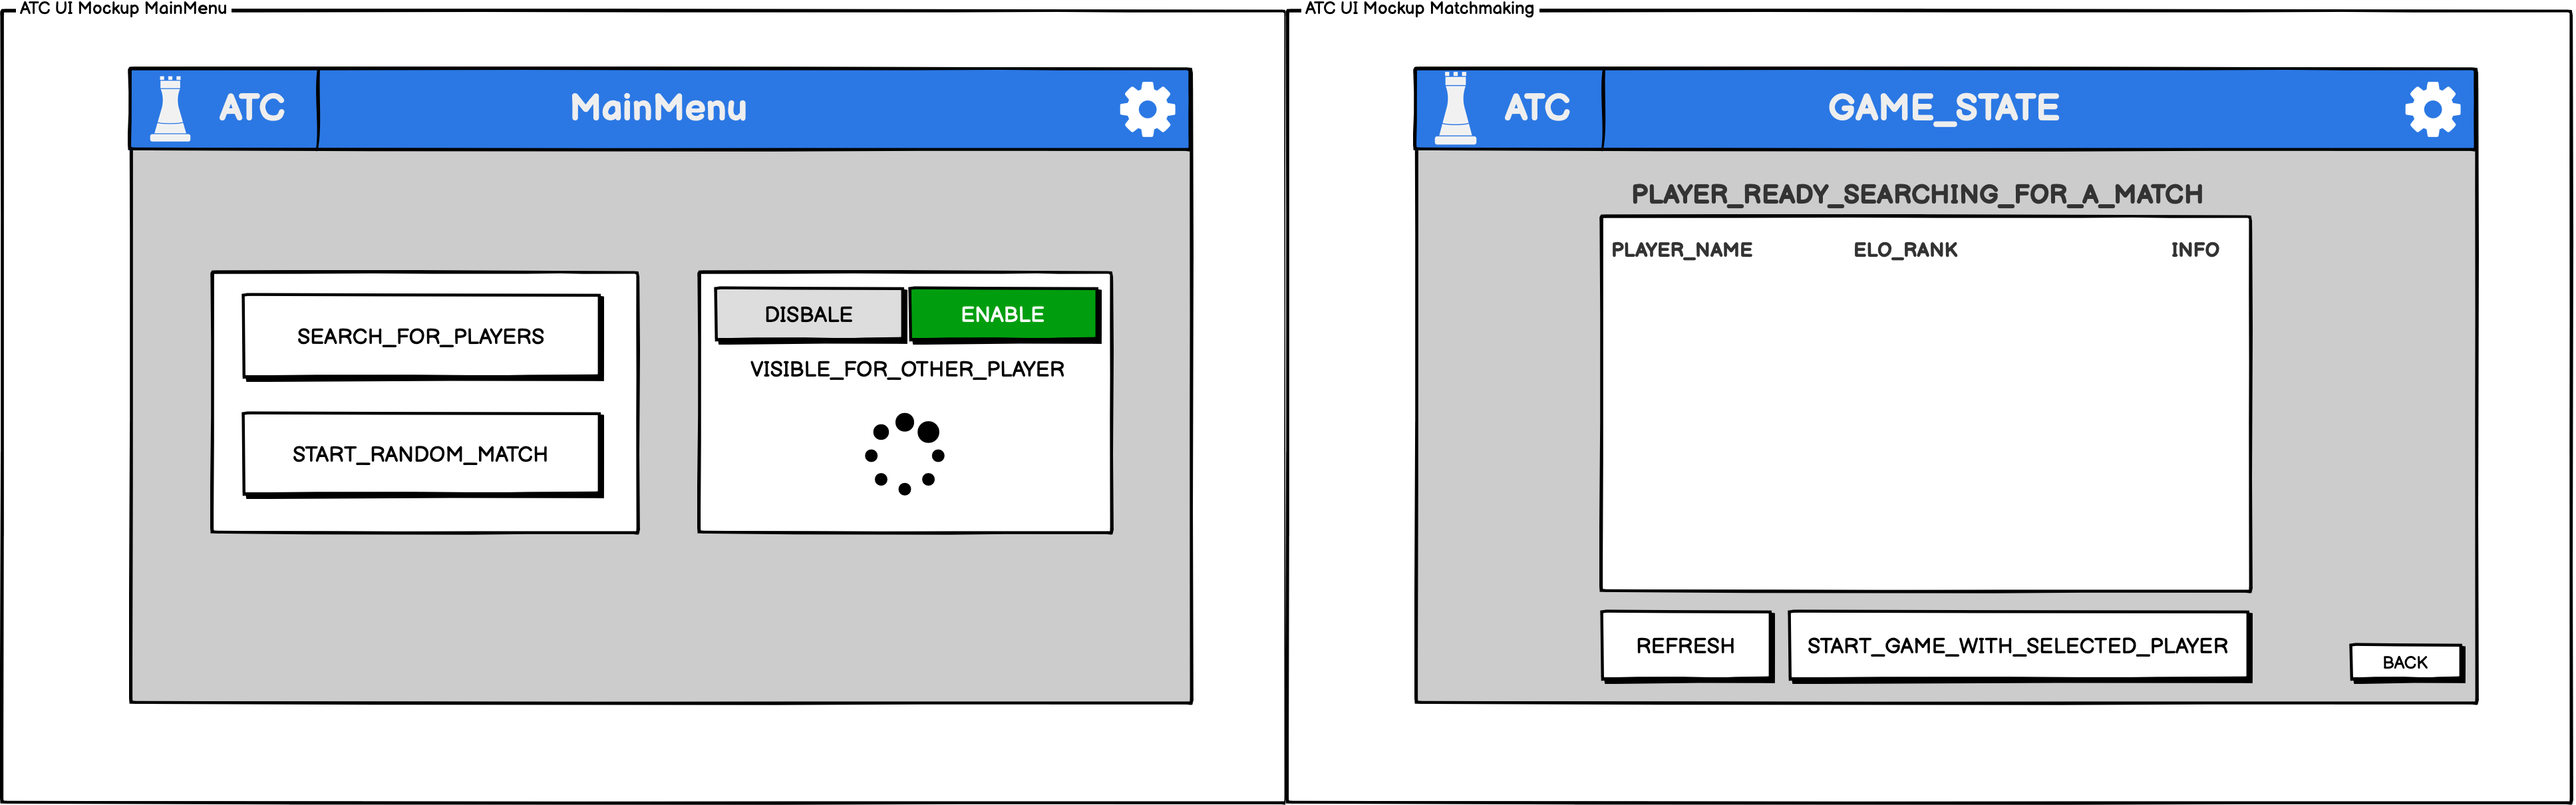
\includegraphics{images/ATC_Gui.png}
\caption{Embedded System Software: User-Interface Mockup
\label{ATC_Gui}}
\end{figure}

Das Qt\cite{qtframework} bietet dazu einen separaten Editor
\passthrough{\lstinline!Qt Design Studio!} an, in denen die zuvor
erstellen Wireframe-Grafiken importiert wurden und anschliessen mit den
Bedienelementen ersetzt werden könnten. Dieser Prozess gestaltete sich
als sehr effizient und so konnte das komplette UI mit moderatem
Zeitaufwand umgesetzt werden.

\begin{lstlisting}
// WINDOW.qml User-Interface ATC
import QtQuick 2.15
import QtQuick.Controls 2.15
//...
Rectangle {
    id: window
    objectName: "window"
    width: 800
    height: 480
    //BACKEND LOGIC INIT => CREATES INSTANCE OF THE MenuManager CLASS
    MenuManager{
        id:main_menu
        objectName: "mainmenu"
    }
    //...
    // MAIN MENU CONTAINER
    Rectangle {
        id: mm_container
        objectName: "mm_container"
        property var headline_bar_name:"Main Menu"
        //START AI MATCH BUTTON
        Button {
                id: mm_start_random_btn
                x: 40
                y: 183
                width: 207
                height: 55
                text: qsTr("START AI MATCH")
                //CONNECT BUTTON EVENTS TO BACKEND LOGIC
                Connections {
                    target: mm_start_random_btn
                    function onClicked(_mouse){
                        //CALL A FUNCTION IN BACKEND LOGIC INSTANCE
                        main_menu.mm_search_for_players_toggled(true)
                    }
                    //...
                }
                //...
\end{lstlisting}

Die anschließende Implementierung der Backend-Logik des Unter-Interface
bestand in der Verbindung, der in \gls{qml} erstellten Bedienelemente
durch den \passthrough{\lstinline!Qt Design Studio!}-Editor und der
User-Interface Backend Logik. Diese beschränkt sich auf die
Initialisierung des Fensters und dem anschließenden laden und darstellen
des \gls{qml} Codes. Die Backend-Logik Funktionalitäten in einem
\gls{qml} Typ \passthrough{\lstinline!MenuManager!} angelegt, welcher
vor dem Laden des eigentlichen User-Interface \gls{qml}-Code registriert
werden muss.

\begin{lstlisting}[language={C++}]
// main.cpp User-Interface ATC
#include <QGuiApplication>
#include <QQmlApplicationEngine>
#include "menumanager.h" //BACKEND LOGIC
int main(int argc, char *argv[])
{
  QCoreApplication::setAttribute(Qt::AA_EnableHighDpiScaling);
  //...
  //CREATE WINDOW
  QWindow window;
  window.setBaseSize(QSize(800,480));

  //REGISTER MainMenu COMPONENT
  qmlRegisterType<MenuManager>("MenuManager",1,0,"MenuManager");
  //LOAD User-Interface QML
  QQuickView view;
  //...
  view.engine()->addImportPath("qrc:/qml/imports");
  view.setSource(QUrl("qrc:/qml/WINDOW.qml"));
  view.engine()->rootContext()->setContextProperty("app", &app);
  //...
  //IMPORTANT STEP: AFTER INIT THE MainMenu COMPONENT HAS NO PARENT
  //SO WE NEED TO SET IT MANUALLY TO MAKE C++ -> QML FUNCATION CALLS WORKING
  QObject *object = view.rootObject();
  QObject *rect = object->findChild<QObject*>("mainmenu");
  if (rect){
         rect->setParent(object);
  }
  //FINALLY SHOW MENU ON SCREEN
  view.show();
}
\end{lstlisting}

Da das User-Interface ein separates Programm ist, welches auf dem System
ausgeführt wird, muss dieses in der Lage sein mit der
Controller-Software zu kommunizieren. Hierzu wurde die zuvor erstellte
\gls{ipc} Bibliothek in das Projekt importiert, jedoch wurde in der
Makefile das \passthrough{\lstinline!USES\_QT!} Define-Flag gesetzt.
Wenn dieses gesetzt ist, wird die Bibliothek in den Client-Modus
versetzt und stellt somit das Gegenstück zu der Instanz dar, welche in
der Controller-Software läuft. Somit werden auch die Funktionen zum
Senden von \passthrough{\lstinline!gui.createEvent()!} umgekehrt, sodass
ein Event in der Controller-Software ausgelöst wird. Dies kann z.B.
durch eine Benutzereingabe oder wenn das User-Interface die von der
Controller-Software geforderten Zustand angenommen hat.

\begin{lstlisting}[language={C++}]
// menumanager.cpp User-Interface ATC
#include "menumanager.h"

MenuManager::MenuManager()
{
    //START IPC THREAD
    guiconnection.start_recieve_thread();
    //...
}

//METHOD CALLED FROM QML ELEMENT ss_calboard_btn
void MenuManager::ss_calboard_btn(){
    //SEND EVENT TO CONTROLLER SOFTWARE
    guiconnection.createEvent(guicommunicator::GUI_VALUE_TYPE::START_CALBOARD_PROC);
}

//PROCESSES EVENTS COMMING FROM THE INTER PROCESS COMMUNICATION AND SHOWS MENUS OR SET IMAGES/LABES
// MenuManager::updateProgress() CALLED BY SPERATE THREAD
void MenuManager::updateProgress()
{
    //GET LATEST EVENT FROM IPC
    const guicommunicator::GUI_EVENT ev =  guiconnection.get_gui_update_event();
    if(!ev.is_event_valid){return;}
    //PROCESS EVENTS
    //SWITCH MAIN MENU REQUEST
    if(ev.event == guicommunicator::GUI_ELEMENT::SWITCH_MENU){
        switch_menu(ev.type);
    }
    //...
}
\end{lstlisting}

\hypertarget{fazit}{%
\chapter{Fazit}\label{fazit}}

Zusammenfassend lässt sich feststellen, dass das Ziel der Arbeit
erreicht wurde. Die Kernfrage, welche die Überprüfung der Ausführbarkeit
inklusive Erstellung und Umsetzung eines eingebetteten Systems und einer
Cloud-Infrastruktur umfasst, konnte abschließend positiv beantwortet
werden.

Es wurde iterativ ein autonomer Schachtisch entwickelt, welcher alle
zuvor gestellten Anforderungen erfüllt. Die Positionen der Schachfiguren
können mittels NFC-Tags in den Füßen der Figuren und eines NFC-Lesers
unterhalb des Schachfelds umgesetzt werden. Die Mechanik zur Bewegung
des NFC-Lesers und eines Magnetes in dessen Mitten ermöglicht zudem
durch gegenpolige Magnete in den Füßen der Figuren ein automatisches
Bewegen der Figuren ohne manuelle Interaktionen. Die Größe des Feldes
ist so ausgelegt, dass Figuren ohne Kontraktionen aneinander
vorbeigeführt und am Rand des Spielfeldes positioniert werden können,
sofern sie aus dem Spiel ausgeschieden sind. Dadurch war eine kleinere
Revision des Tisches nicht anwendbar, dennoch konnten mittels der
größeren Dimensionen der letzten Revision diese Funktion und weitere,
wie die Mechanik zur Bewegung, optimiert und adäquater umgesetzt werden.

Der Tisch verfügt über eine Stand-Alone Funktionalität, welche das
Starten und Auswerten eines Spiels ohne Anbindung zum Internet oder zu
externen Geräten, wie eines Smartphones, ermöglicht. Dennoch ist es über
eine Verbindung zum Internet mittels eines Cloud-Services möglich,
zusätzliche Funktionen wie das Spiel gegen andere, reale Spieler oder
gegen eine Schachlogik zu nutzen oder einen Livestream zum Darstellen
von gegenwärtigen Spielen aufzubauen.

Anhand der Durchführung von iterativen Verbesserungen und einzelnen
Revisionen des Modells lassen sich definierte Aussagen zu Fortschritten
und Veränderungen des Gesamtsystems treffen. Der Schachtich als
eingebettetes System besteht aus einem modularen Aufbau, welches sich im
Verlauf der Iterationen durch das Anpassen einzelner Komponenten
aufwerten ließ. Derartige Systeme erfordern in der Vorbereitung ein
hohes Verständnis der Zusammenhänge von Komponenten, da spätere
Veränderungen komplexer sind; da hierbei in den verschiedenen
Iterationen aber nur einzelne Modulgruppen verändert wurden, musste
lediglich die Verbindung des jeweiligen Moduls neu berücksichtig werden
und keine gänzliche Aufwertung aller Komponenten erfolgen. Anders als
Mehrzwecksystemen, welche oftmals weniger einzelne Module beinhalten,
konnte hier eine separierte Betrachtung der Komponenten erfolgen.

Nicht nur der Aufbau der Komponenten erfolgt modular, sondern auch das
Erstellen allen Softwarekomponenten und die Konstruktion des
Schachtischt. Letzteres führt zu einem einfachen Aufbau des Tisches,
welcher auch von versierten oder motivierten Anwendern ausgeführt werden
könnten. Eine aussagekräftige Versuchsführung dazu liegt jedoch nicht
vor. Zudem sind nahezu alle verwendeten Materialien mühelos erhältlich,
nur 3D-Komponenten müssen separat gedruckt werden. Die alle Ressourcen
einschließlich der \gls{cad} -Modelle sind online zur Verfügung gestellt
worden.

Die Bedienung des Systems mittels des verbauten Bildschirms ist
ebenfalls auf eine simple Benutzerführung spezifiziert. Auch unerfahrene
Spieler können ein Spiel beginnen ohne eine differenzierte Einweisung
erhalten zu haben. Diese Funktionalität wurde an einzelnen Probanden
getestet, eine aussagekräftige Statistik liegt jedoch nicht vor.

Grundsätzlich ist festzuhalten, dass es sich beim Resultat der Arbeit um
kein finalisiertes Produkt, sondern um einen strukturellen Prototyp
handelt. Weitere Prüfungen, wie Nutzungsstatistiken oder
Sicherheitsprüfungen, müssten durchgeführt werden, ehe der Schachtisch
als kommerzielles Produkt betrachtet werden kann. Auch fehlen diverse
Langzeittests. Ein Betriebstest mit einer Dauer von 6 Stunden verlief
ohne erkennbare Zwischenfälle, für aussagekräftige Verschleiß- und
Fehlererkennungen bedarf es jedoch noch weiterer und längerer
Untersuchungen.

Der Prototyp lässt sich jedoch mit kommerziell erhältlichen und
open-source verfügbaren Schachtischen vergleichen. Das Ziel, alle
wünschenswerten Funktionen und Implementationen dieser Tische in den
Prototypen zu integrieren, konnten erfolgreich umgesetzt werden. Darüber
hinaus wurde weitere Funktionalitäten eingegliedert, wie eine
Stand-Alone Funktionalität oder einer Schnittstelle zum Erstellen
weiterer Erweiterungen.

Das System und insbesondere der implementierte Cloud-Service sind online
erreichbar und erweiterbar. Dies ermöglicht unter anderem das Bauen
eines eigenen Tisches unter der Verwendung des AtomicChess Systems, aber
auch die Integration weiterer Komponenten. Erfahrene Entwickler können
somit das Spiel beliebig ausweiten oder sogar andere Spiele ergänzen.
Die für das Projekt entworfene Mechanik und Spielführung kann
dementsprechend auch für diverse andere Tischbrettspiele verwendet
werden.

Neben diversen im Studium erlernten Fähigkeiten wurden im Laufe des
Projekts noch diverse andere Leistungen erforderlich, wie die Erstellung
einer Mechanik oder das Konstruieren von Komponenten, welche das
Aneignen von zusätzlichem Wissen erfordern. Die resultierende Mechanik
ist ungeachtet dessen ist fehlerlos und nahezu spielfrei, was ein
reibungsloses Spiel ermöglicht

Abschließend lässt sich feststellen, dass ein funktionstüchtiger
Schachtich konstruiert wurde, der basierend auf einem eingebetteten
System und einer Cloud-Infrastruktur als gelungener Abschluss eins
Informatikstudiums bezeichnet werden kann.

\hypertarget{persuxf6nliches-fazit}{%
\section{Persönliches Fazit}\label{persuxf6nliches-fazit}}

Im Verlauf dieser Arbeit bin ich persönlich weit über mich
hinausgewachsen und ich bin sehr stolz, mein fertiges Projekt
präsentieren zu können. Ich konnte nicht nur theoretisch die Machbarkeit
meines Konzepts beweisen, sondern auch einen physischen Prototypen
erstellen.

Natürlich bietet das System noch schwächen und Bedarf diverser
Ergänzungen, bevor man es als Produkt betrachten kann. Dazu gehören auch
diverse Untersuchungen, wie ein Langzeittest oder schleifenbasierte
Hardwareüberprüfungen. Es wäre von Vorteil gewesen, das System durch
einen erfahrenen Schachspieler bewerten zu lassen oder Rückmeldung über
die Struktur und Menüführung von Anfängern zu erhalten. Diese Option
blieb aufgrund von Versammlungs- und Zusammentreffens-Reglementierungen
jedoch verwehrt. Für eine vollständige Analyse fehlen daher wichtige
statistische Daten.

Doch genau solche Erkenntnisse geben mir einen Anreiz, das Projekt auch
nach Abschluss des Studiums nicht zu beenden, sondern weitere Ideen
umzusetzen und anschließend auch mit Testpersonen zu erproben.

Der iterative Prozess der Erstellung des Schachtichs ist zeitaufwändig
und kostspielig, ermöglicht allerdings das frühzeitige Erkennen von
Schwachstellen und das Ausbessern der jeweiligen modularen Komponente,
noch eher eine Etablierung im System erfolgen kann. Ebenso ermöglicht es
ein einfacheres Verständnis über alle Komponenten, lediglich die
Zusammensetzung und Beziehung dieser muss rechtzeitig überdacht werden.

Insgesamt ist das Projekt selbst recht umfangreich und umfasst in
verschiedenen Facetten diverse Themenbereiche meines Studiums, was mir
von Beginn an ein Anliegen war. Es manifestiert meinen
Studienschwerpunkt, die technische Informatik, und hat mich dazu
verleitet, noch tiefgründiger in die Materie zu schauen. Zudem wurden
noch weitere Kompetenzen erfordert, welche zuvor gar nicht oder nur
teilweise gegeben waren, wie das Konstruieren von 3D-Komponenten oder
das Gestalten von Produkten. Umso beeindruckter bin ich selbst von der
Bewegungsmechanik des Systems, welche sich im Entwicklungsprozess sehr
stark verändert hat und letztlich zu einem fehlerlosen Resultat führte.

Neben diesen projektspezifischen Kompetenzen ist es zudem möglich
gewesen, weitere Erfahrungen im Bereich der Projektplanung und
Organisation zu sammeln. Im optimalen Verlauf wäre ein fertiger Prototyp
bereits zum Ende des Winters möglich gewesen, jedoch erforderte die
Veränderung der Mechanik vom XY-System zu CoreXY und verschiedene
unvorhergesehene Schwächen mit den verwendeten Magneten weitere
Umsetzungsiterationen, die Rückblickend nötig und zielführend waren.

Auch die Erstellung der Thesis und das Formatieren von Vorlagen und
Befehlen in Markdown und Latex erwies sich als lehrreich und innovativ.

Insgesamt bin ich sehr zufrieden mit meinem Ergebnis, aber auch mit mir
selbst und meiner erbrachten Leistung.

\hypertarget{ausblick}{%
\section{Ausblick}\label{ausblick}}

Wie jedes Produkt und insbesondere jeder Prototyp nach Abschluss eines
Projekts lassen sich auch hierbei Aussagen zu Verbesserungen und
Ergänzungen tätigen.

In erster Linie besteht die Möglichkeit, diversen Modifikationen des
traditionellen Schachs in das System zu integrieren. Diese Option wurde
im Laufe des Projekts bewusst ausgelassen. Doch auch Erweiterungen auf
diverse andere Brettspiele, wie beispielsweise Mühle, Dame oder
Mensch-ärgere-dich nicht wären optional möglich. Mittels eines
bildgebenden Systems oberhalb des Tisches oder Lichtelementen und
Strukturen unterhalb einer durchsichtigen Tischplatte wäre es möglich,
diverse Strukturen anzuzeigen und als Spielbrett darzustellen.

Auch weitere Hardware kann mittels Porterweiterungen wie \gls{usb} zum
Tisch ergänzt werden. So wäre zum Beispiel eine Schachuhr optional,
welche bei öffentlichen Turnieren erforderlich ist. Eine Uhr würde zudem
erkenntlich machen, wann ein Spieler den eigenen Zug beendet hat.
Derzeit geschieht dies über eine Nutzereingabe oder bei Ablauf eines
Timers.

Zudem ermöglicht die Verbindung zum Internet unzählige Kapazitäten, wie
die Einbindung anderer, existierender Schach-Clouds wie beispielsweise
„licchess.org``.

Ebenso könnten Sprachassistenten ergänzt werden, die das Spiel somit
auch für körperlich eingeschränkte Personen möglich macht. Diese könnten
zudem auch über aktuelle Zustände auditiv informieren oder weitere
Befehle berücksichtigen.

Der derzeitige Systemzustand ermöglicht ein autonomes Schachspiel mit
möglichst äquivalentem Spielerlebnis im Vergleich zu einem
konventionellen Schachspiel. Auf Basis dessen ist der Anzahl der
möglichen Ergänzungen und Ideen zur Verbesserung sind keine Grenze
gesetzt. Erfahrene Entwickler ist die Möglichkeit geboten, diese mittels
der diversen Schnittstellen eigenständig zu integrieren. Das System als
solches ist dennoch ein abgeschlossenes Projekt mit einem präsentablen
Resultat.


